\documentclass[en]{pracamgr}

\usepackage[autostyle]{csquotes}
\usepackage{blindtext}
\usepackage{algorithm}
\usepackage{algpseudocode}
\usepackage{amssymb}
\usepackage{caption}
\usepackage{hyperref}
\usepackage{bookmark}
\usepackage{graphicx}
\usepackage{minted}
\usepackage{amsmath}
\usepackage{booktabs}
\usepackage{multirow}
\usepackage{adjustbox}
\usepackage{csquotes}

\usepackage[backend=biber,style=apa,natbib=true]{biblatex}
\addbibresource{zotero.bib}
\addbibresource{other.bib}

\usepackage{./cite_hyper_fix}

\AtEveryBibitem{
    \clearfield{urlyear}
    \clearfield{urlmonth}
}

\newcommand{\algorithmautorefname}{Algorithm}
\newcommand{\listingautorefname}{Listing}
\newcommand{\env}[1]{{\tt #1}}
\newcommand{\figurewidth}{\linewidth}
\newcommand{\figureheight}{0.8\paperheight}

\DeclareMathOperator*{\argmax}{arg\,max}
\DeclareMathOperator*{\argmin}{arg\,min}
\DeclareMathOperator*{\clip}{clip}

\begin{document}

\autor{Jakub Bednarz}{406103}

\title{Investigating and Combining Approaches for Data-Efficient Model-based RL}
\titlepl{Analiza i połączenie metod w wydajnym obliczeniowo uczeniu ze wzmocnieniem  bazowanym na modelu}

\kierunek{Machine Learning}

\opiekun{dr. Jacek Cyranka\\
  Instytut Informatyki\\
}

\date{Nov 2024}

\dziedzina{%
  11.4 Artificial Intelligence\\
}

\klasyfikacja{%
  I. Computing methodologies\\
  I.2. Artificial Intelligence\\
  I.2.6. Learning
}

\keywords{deep learning, reinforcement learning, model-based, sample-efficient RL}

\maketitle

\begin{abstract}
  Many approaches for data-efficient reinforcement learning (RL) have been developed in the recent years. This paper examines the state of the field, selects an array of such modifications, and provides a framework for incorporating them into a model-based RL agent. Our experiments show, that an RL agent competitive on Atari-100k benchmark can be developed in such a fashion. A custom PyTorch-based RL framework for training modular and highly configurable agents is developed. The source code is available at \url{https://github.com/vitreusx/rsrch}
\end{abstract}

\tableofcontents

\chapter{Introduction}

Reinforcement Learning (RL), a research field dedicated to developing intelligent autonomous agents, capable of learning to do tasks in various environments \autocite{sutton2018reinforcement}, has achieved remarkable progress in recent times. Through the use of deep learning and artificial neural networks, algorithms playing complex games at a super-human level, such as Atari \autocite{mnihHumanlevelControlDeep2015}, Go \autocite{silverMasteringGameGo2016}, Dota 2 \autocite{openaiDota2Large2019}, or StarCraft II \autocite{vinyalsGrandmasterLevelStarCraft2019}, as well as controlling robots \autocite{openaiSolvingRubiksCube2019,brohanRT1RoboticsTransformer2023} and finetuning Large Language Models from human feedback \autocite{ouyangTrainingLanguageModels2022}, have been developed.

However, most of the current state-of-the-art techniques have a significant drawback: they require excessive amounts of data (which, in this setting, we regard as the total time spent interacting with the environment) in order to achieve such performance. For example, the standard benchmark on a collection of Atari video games \autocite{bellemareArcadeLearningEnvironment2013} assumes a total interaction budget of 200 million game frames, equivalent to a single person playing for $\approx 40$ days without rest. For playing Dota 2, thousands of years in total are required. This shortcoming greatly limits real-world deployment of such methods. Simulation of the target environment is often not available, and even in the presence of such models, the inaccuracies cause the policies developed in simulation to not transfer completely to the real world. There may also arise additional safety considerations \autocite{yampolskiy2018artificial}, forcing us to constrain the number of interactions to a minimum.

In order to remedy this problem, many approaches designed with \emph{sample efficiency}, being the maximization of agent performance in a given (small) number of interactions with the environment, in mind, have been proposed. Arguably the most appealing method is to learn a model of the environment, in order to predict the future or possible future events. Such approaches are called \emph{model-based} RL, as opposed \emph{model-free} RL, in which such a model is not learned. Through it, an optimal policy can be learned without any interactions with the real environment. The model can also be used for directed exploration \autocite{sekarPlanningExploreSelfSupervised2020} or transfer to novel tasks \autocite{byravanImaginedValueGradients2019}. Indeed, a number of data-efficient architectures have been developed using the world models in this capacity, via lookahead search \autocite{schrittwieserMasteringAtariGo2020,yeMasteringAtariGames2021} or learning policies purely from synthetic data \autocite{haRecurrentWorldModels2018,hafnerDreamControlLearning2020,kaiserModelBasedReinforcementLearning2024,hafnerMasteringDiverseDomains2024}. Learning an accurate world model from a small number of samples is difficult, however, and training a policy with it can lead to model exploitation \autocite{kurutachModelEnsembleTrustRegionPolicy2018}, whereby the policies exploit inaccuracies in the learned model and fail to perform well in the real environment. The overhead of having to learn the model also leads to increased compute requirements of the agents.

There have, however, been efforts conducted to render learning the policy sample-efficient without the use of environment modelling. One line of research, for example, attempts to simply optimize the training recipe, e.g. the number of optimization steps per single environment interaction, without changing either the RL algorithm used, or the architecture \autocite{doroSampleEfficientReinforcementLearning2022,schmidtFastDataEfficientTraining2021}. Other works introduce data augmentation \autocite{kostrikovImageAugmentationAll2021,yaratsMasteringVisualContinuous2021}, self-supervised learning \autocite{schwarzerDataEfficientReinforcementLearning2021} or using larger neural network backbones \autocite{hafnerMasteringDiverseDomains2024,schwarzerBiggerBetterFaster2023}.

All these have resulted in significant improvements in terms of sample efficiency. Many of these innovations have been developed independent of each other, however, and in many cases are orthogonal, meaning it is possible to envision a single RL agent combining many such strategies and modifications, possibly capable of reaching even higher performance than standalone algorithms. A similar feat has been achieved by the Rainbow agent \autocite{hesselRainbowCombiningImprovements2017}, which augments a base RL architecture DQN \autocite{mnihHumanlevelControlDeep2015} with an array of small modifications, which turn out to provide significant boost to the base agent in terms of final performance. Works such as BBF \autocite{schwarzerBiggerBetterFaster2023} have shown, that such an approach can also be used to increase sample efficiency of the agents, in the model-free scenario.

The goal of this thesis is to investigate whether this can be achieved for sample-efficient model-based RL. To be precise, our goal is to take a model-based architecture, originally not designed with data efficiency in mind, and use the ideas developed in other works, mostly in the context of model-free RL, to see whether one can achieve significant performance benefits without any major architectural interventions. Specifically, we base our work on DreamerV2 \autocite{hafnerMasteringAtariDiscrete2022}, which has been developed for the Atari-200m benchmark \cite{bellemareArcadeLearningEnvironment2013}, with a set of 55 Atari games and a time limit of $200 \times 10^6$ environment steps. So far, it has not been studied, whether recently proposed SOTA improvements in sample efficiency are suitable in a model-based setting. Compared with the next iteration DreamerV3, which achieves sample efficiency through scaling the world model and applying robustness techniques based on e.g. reward normalization, we attempt to develop a more general approach for creating sample-efficient agents, with plug-and-play features that can be used across different world model designs.

In summary, our principal contributions are:

\begin{enumerate}
  \item An open source, highly customizable and modular model-based RL framework. Our framework is the first to allow for a systematic ablation study of applying recent advances in RL data efficiency to a model-based agent. Our library is implemented in PyTorch \autocite{paszkePyTorchImperativeStyle2019}, which is the most popular library for Deep Learning currently.
  \item An in-depth analysis of the effects of state-of-the-art improvements in sample efficiency for a model-based architecture, such as training recipe optimization, performing data augmentation, and using better RL algorithms.
  \item A sample-efficient model-based RL agent architecture, comparable with state-of-the-art model-based data-efficient RL architectures, such as IRIS \autocite{micheliTransformersAreSampleEfficient2023}, TWM \autocite{robineTransformerbasedWorldModels2023} or DreamerV3 \autocite{hafnerMasteringDiverseDomains2024} in terms of human-normalized mean performance on Atari-100k benchmark ($0.975$ for our agent, $1.046$ for IRIS, $0.960$ for TWM, $1.250$ for DreamerV3).
\end{enumerate}

The rest of the thesis is structured as follows. First, we perform the literature review, in order to assess what are the existing methods for improving data efficiency of RL agents. We identify the finetuning the training recipes, applying data augmentations, and changing the RL algorithms used in model-based RL as the most promising developments to incorporate into our design. We propose how to combine them into a single RL agent, and design empirical studies aimed at investigating the effects of the ablations, and the changes in terms of agent performance.

After having considered a number of existing RL frameworks, and deeming them unsuitable for the purpose of conducting our study, due to lack of support for various improvements reported in literature like data augmentation, or update ratio adjustment, we design and implement a novel PyTorch-based \autocite{paszkePyTorchImperativeStyle2019} RL framework capable of facilitating our experiments. We describe how different design choices help with making the framework as flexible, yet user-friendly, as possible, and highlight the advantages our solution has over other model-based RL frameworks, such as the support for recent SOTA features that helped to improve other RL algorithms in a plug-and-play fashion and the ability to conduct comprehensive ablation studies. We make the framework and all the code necessary to replicate the experiments conducted in this thesis publicly available at \href{https://github.com/vitreusx/rsrch}{\tt vitreusx/rsrch}.

Then, we will follow up with the execution of the experiments, and the analysis of the results. We discover that the design of the training loop, and the use of improved RL modules yield greatest improvements in terms of the final performance of the agent. On the other hand, otherwise promising avenues, such as the use of data augmentation, prove ultimately unsuccessful in improving the algorithm, and can even significantly degrade the policies learned.

Having in mind the number of hyperparameters which such a modular design introduces, we also employ and analyze methods for auto-tuning some of them. Specifically, following \autocite{dorkaDynamicUpdatetoDataRatio2023}, we implement and improve upon a mechanism for automatically adjusting optimization frequency based on the model validation loss.

Throughout, we provide a detailed analysis of the learning dynamics and the behavior of the trained agents, in order to elucidate the causes of the observed performance improvements and hits, as well as better direct our efforts towards further modifications to discuss and test.

Finally, we use these findings to implement an RL agent using these modifications in tandem, and verify that the combination yields a further improvement in terms of validation scores achieved. We then test the best-performing configuration on Atari-100k benchmark, a standard benchmark for visual sample-efficient RL algorithms, and compare it with other state-of-the-art solutions. We find, that the performance is comparable with some of the state-of-the-art model-based data-efficient RL architectures, as indicated by the human-normalized mean performance.

\chapter{Preliminaries}

\section{Reinforcement Learning}

Reinforcement Learning is a field of artificial intelligence and machine learning concerned with constructing intelligent agents capable of learning what actions to take in an environment so as to maximize a scalar reward signal \autocite{sutton2018reinforcement}.

Formally, the environment can be represented by a Markov decision chain (MDP) in the form of a tuple $\langle \mathcal{S}, \mathcal{A}, p \rangle$ consisting of the state space $\mathcal{S}$, action space $\mathcal{A}$ and transition probability $p(s_{t+1}, r_{t} \mid s_t, a_t)$, where $r_t \in \mathbb{R}$ denotes the reward granted at that step. Additionally, in the case of partially observable environments, we have an observation space $\mathcal{O}$ and an observation probability $p(o_t \mid s_t)$. The agent, starting from an initial observation $o_1$, acts according to a probability distribution $\pi(a_t \mid o_{\leq t})$ conditioned on previous observations until it reaches a \emph{terminal} state $s_T$. The goal of reinforcement learning and the RL agent is to maximize the expected sum of rewards (so called returns) obtained along the trajectory $J = \mathbb{E} \left\{\sum_{t=1}^{T-1} r_t\right\}$.

There are two further quantities of interest. The state value function $V^\pi(s)$ equal to the expected returns of an agent acting with a policy $\pi(a_t \mid s_t)$, when starting from a state $s$. The state-action value function $Q^\pi(s, a)$ (called thereafter $Q$ function) equal to the expected returns of an agent acting with a policy $\pi$, when starting from a state $s$ and having just performed action $a$. These value functions are usually $\gamma$-discounted: rather than using the returns $\mathbb{E} \left\{\sum_{t=1}^{T-1} r_t\right\}$, we consider $\mathbb{E} \left\{\sum_{t=1}^{T-1} \gamma^{t-1} r_t\right\}$ for $0 < \gamma < 1$.

One approach towards learning behavior in an environment is \emph{Q-learning}. The idea is as follows: we want to learn an optimal policy $\pi^*$ such, that $V^{\pi^*}$ is maximized for all states $s$. It is clear, that such a policy should choose $a$, which maximizes $Q^{\pi^*}(s, a)$, i.e. $\pi^*$ should be deterministic, and return $\pi^*(s) = \argmax_a Q^{\pi^*}(s, a)$. It can be shown, that such a policy, and such an induced $Q$-function $Q^{\pi^*} =: Q^*$ satisfy $Q^*(s, a) = \mathbb{E}_{s'} \left\{r + \gamma Q^*(s', \pi^*(s'))\right\}$. This recurrence relation allows us, in turn, to learn the value of $Q^*$ through fixed-point iteration.

A different way to learn optimal behavior is to learn the policy directly, rather than construct it from $Q$-value estimates, by taking a gradient of the returns and using standard first-order optimization methods. Specifically, by the policy gradient theorem \autocite{suttonPolicyGradientMethods1999}, we have $\nabla_\theta J = \mathbb{E}\left[\sum_t \Psi_t \nabla_\theta \log{\pi_\theta(a_t \mid s_t)}\right]$ for an on-policy sequence $(s_{1:T+1}, a_{1:T}, r_{1:T})$, where $\Psi_t$ can be e.g. total trajectory returns $J$, state-action value $Q(s_t, a_t)$, or an \emph{advantage value} $Q(s_t, a_t) - V(s_t)$.

\subsection{Deep RL}

The advances in deep learning have allowed components such as $Q$ or value functions, and policies, to be realized as expressive function approximators, leading to breakthroughs in settings hitherto considered unsolvable. In a foundational work, \autocite{mnihHumanlevelControlDeep2015} have designed a $Q$-learning-based agent DQN, reaching human-level performance on a suite of Atari video games. Actor-critic methods, such as Deep Deterministic Policy Gradients (DDPG) \autocite{lillicrapContinuousControlDeep2019} and Soft Actor Critic (SAC) \autocite{haarnojaSoftActorCriticOffPolicy2018} have extended this approach to continuous action spaces. Methods based on policy gradients, such as Trust Region Policy Optimization (TRPO) \autocite{schulmanTrustRegionPolicy2017} and Proximal Policy Optimization (PPO) \autocite{schulmanProximalPolicyOptimization2017}, have also been developed.

\section{Sample-efficient RL}

Works such as DQN have reached human-level performance in arcade by playing an equivalent of $\approx 38.5$ days ($200 \times 10^6$ frames with frame rate of $60$ FPS). Even with a simulator available, the excessive number of data required by standard RL algorithms can prove troublesome, as in the case of OpenAI Five \autocite{openaiDota2Large2019}, which had to be trained for 10 months on an entire distributed system, and required development of sophisticated ``surgery'' techniques due to having to restart training at multiple points in time. In domains such as robotics, this kind of scaling quickly becomes prohibitively expensive and time-consuming. Thus, developing sample-efficient methods is necessary to allow the deployment of deep RL agents in real environments.

\subsection{Benchmarks for data-efficient RL}

In order to gauge progress in sample-efficient deep RL, a number of standardized benchmarks have been proposed.

\paragraph{Atari-100k} For discrete control, the \emph{de facto} standard benchmark is Atari-100k \autocite{kaiserModelBasedReinforcementLearning2024}, a subset of 26 games from the full Atari Learning Environment \autocite{bellemareArcadeLearningEnvironment2013} benchmark, limited to $400\times 10^3$ game frames, equivalent to $100 \times 10^3$ agent steps, assuming the standard practice of repeating every agent's action $4$ times.

\paragraph{DMC} For image-based continuous control, the most widely used benchmark has been DeepMind Control suite \autocite{tassaDeepMindControlSuite2018} limited to either $100 \times 10^3$ or $500 \times 10^3$ agent interactions, as proposed in \autocite{kaiserModelBasedReinforcementLearning2024}. This setup has been used by e.g. \autocite{kostrikovImageAugmentationAll2021,srinivasCURLContrastiveUnsupervised2020}.

\section{Model-based RL}

Whereas a model-free RL agent seeks only to learn the policy $\pi$, either directly or indirectly through a $Q$ function, a model-based agent seeks also to simulate the environment itself and be able to predict the future, in order to aid learning the policy, or avoid having to do it altogether \autocite{sutton2018reinforcement}.

\subsection{Learning the model}

Most model-based RL algorithms aim to predict future stats or observations. SimPLE \autocite{kaiserModelBasedReinforcementLearning2024} performs the transition in input (image) space - the UNet-like model receives input consisting of last $K$ frames, as well as action conditioning, and is trained to output next frame. The main issue with this approach is that encoding and decoding images in such a fashion proves to be computationally expensive. Indeed, the training time is $5$ A100-days (as reported by \autocite{hafnerMasteringDiverseDomains2024}). Thus, other model often opt to perform modelling in the latent space. World Models \autocite{haRecurrentWorldModels2018}, for example, uses a two-stage training recipe: visual inputs are first compressed into a latent vector using a Variational Autoencoder \autocite{kingmaAutoEncodingVariationalBayes2022}, whereafter a combination of an RNN and a ``distribution head'' model the transition probabilities in the latent space. In the context of PlaNet agent \autocite{hafnerLearningLatentDynamics2019}, the authors raise the issues surrounding modelling stochastic environments autoregressively, and propose the use of both deterministic and stochastic recurrent networks in order to deal with stochasticity without inducing the decay of the information stored in the state vector. This approach has been further refined in the Dreamer series of models \autocite{hafnerDreamControlLearning2020,hafnerMasteringAtariDiscrete2022,hafnerMasteringDiverseDomains2024} by e.g. using discrete latent states, employing better techniques for learning prior and posterior state distributions, or improving critic learning through the use of value distributions \autocite{bellemareDistributionalPerspectiveReinforcement2017}. IRIS \autocite{micheliTransformersAreSampleEfficient2023} uses a VQ-VAE \autocite{oordNeuralDiscreteRepresentation2018} to encode input observations into a sequence of discrete tokens, and a GPT-like Transformer architecture \autocite{vaswaniAttentionAllYou2017} to predict future tokens, along with rewards and episode-end indicators. MBPO \autocite{jannerWhenTrustYour2021} uses a bootstrap ensemble of individual dynamics models in order to model aleatoric and epistemic uncertainties, and better prevent model exploitation.

Model states do not necessarily need to correspond to real states - in the case of \emph{value-equivalent models}, the states and the transition function are optimized to approximate the values to be obtained after executing a sequence of actions \autocite{silverPredictronEndToEndLearning2017}. The idea is to construct an abstract MDP, in which planning is equivalent to planning in the real environment. This way, model capacity is wholly used for the purposes of learning the policy, as opposed to modelling potentially irrelevant details. TreeQN \autocite{farquharTreeQNATreeCDifferentiable2018}, for example, learns a differentiable, recursive, tree-structured model acting as a replacement for the $Q$ function in arbitrary model-free RL algorithm. In MuZero \autocite{schrittwieserMasteringAtariGo2020}, the model is optimized to jointly predict rewards, the action-selection policy, and the value function, leading to an agent capable of learning to play Atari, Go and chess at a superhuman level. EfficientZero \autocite{yeMasteringAtariGames2021} adapts MuZero for sample-efficient image-based RL, through addition of self-supervised consistency loss \autocite{chenExploringSimpleSiamese2020}, refinements in reward and value prediction, and a method to correct off-policy issues when using replay buffer samples to compute value targets.

\subsection{Using the model}

One class of methods uses the model for \emph{planning}; such techniques are also known as \emph{lookahead methods}. Here, planning refers to any decision process which actively uses the world model. For example, in its simplest incarnation, Model-Predictive Control (MPC), at every time step, optimizes a sequence of actions $a_t, \ldots, a_{t+H-1}$ such that the expected total rewards $\mathbb{E}\left\{\sum_{k=0}^{H-1} r_{t+k} \right\}$ is maximized, and selects the first action $a_t$ - at the next step, the procedure is performed again. The action sequence can be optimized using any zero-order method, like Monte Carlo (i.e. sampling the actions randomly and selecting the one with the best score), or through Cross-Entropy Method (CEM). A variation of this idea is to employ a Monte Carlo Search Tree in order to focus on more promising directions of exploration. In all cases, an auxiliary value function predictor can also be used in order to approximate the returns beyond the rollout horizon.

At the other end of the spectrum lay approaches which use model rollouts for learning the policy. Such rollouts can then be used to completely replace training on real data, instead learning behaviors entirely in the ``imagination'' via regular model-free RL algorithms, as in the Dreamer series of algorithms \autocite{hafnerDreamControlLearning2020,hafnerMasteringAtariDiscrete2022,hafnerMasteringDiverseDomains2024} or MBPO \autocite{jannerWhenTrustYour2021}. Due to the differentiability of the world model, one can also perform backpropagation of values through dynamics gradients directly \autocite{hafnerDreamControlLearning2020}.

\section{Data augmentation in RL}

Drawing from the common practice of using data augmentation (e.g. image transformations like rotation, random shifts) in supervised learning to improve performance and reduce overfitting, there exist also methods, which apply these techniques in the context of RL. RAD \autocite{laskinReinforcementLearningAugmented2020} apply transforms, such as cropping, translation, conversion to grayscale or color jitter, to SAC and PPO. DrQ \autocite{kostrikovImageAugmentationAll2021} develops an RL-specific augmentation schema: beyond simply applying random transforms to observations, the authors also use the fact, that $Q$ and state-value functions ought to be invariant with respect to the transforms to smooth them out by averaging across multiple samples. In robotics, domain randomization has become a crucial component of transfering policies trained in simulation to the real world \autocite{tobinDomainRandomizationTransferring2017,openaiSolvingRubiksCube2019}.

\section{Self-supervised RL}

Standard deep RL methods, such as DQN or SAC, only utilize the reward signal in order to learn useful state representations to be used to learn the policy. Some authors have proposed employing techniques from the area of self-supervised learning (SSL) in order to combat this inefficiency.

Broadly speaking, self-supervised learning consists of adding additional \emph{pretext tasks}, which are solved not for their own sake, but rather to provide learning signal for the downstream representations. Many kinds of pretext tasks have been suggested:

\begin{itemize}
  \item For visual input, one option is to exploit inherent structure of images, via rotation prediction \autocite{gidarisUnsupervisedRepresentationLearning2018}, colorization (reconstructing the image from a grayscale version) \autocite{zhangColorfulImageColorization2016} or jigsaw (splitting an image into patches, randomizing the order and reconstructing the original image) \autocite{norooziUnsupervisedLearningVisual2017}.
  \item Contrastive learning (CL) approaches, based on the instance discrimination task, construct such representations, that views (augmentations, crops etc.) of the same instance (``positive pairs'') are pulled together, and views of different instances (``negative pairs'') are pulled apart \autocite{chopraLearningSimilarityMetric2005,schroffFaceNetUnifiedEmbedding2015}. Some CL methods do not use negative pairs altogether, relying on momentum, batch normalization and projection heads to avoid collapse of the representations \autocite{grillBootstrapYourOwn2020}.
  \item Generative approaches reconstruct input from noisy or corrupted versions. Autoencoders, variational autoencoders (VAEs) and denoising VAEs \autocite{inproceedings} pass the (possibly augmented) input through a latent bottleneck in order to recover the original input. The corruption can also take form of masking patches of the input - this approach has proven especially suited to pre-training representations for NLP \autocite{devlinBERTPretrainingDeep2019} and Vision Transformers \autocite{heMaskedAutoencodersAre2021}.
\end{itemize}

Similarly, self-supervised RL techniques attempt to incorporate pretext tasks into regular RL pipelines. Arguably the simplest way is to apply SSL to augment learning of observation embeddings. For example, CURL \autocite{srinivasCURLContrastiveUnsupervised2020} takes a base RL model (in this instance SAC) and uses MoCo \autocite{heMomentumContrastUnsupervised2020} to help train the observation encoder via an auxiliary CL loss term. Some architectures, however, design the pretext task to be more RL-specific. SPR \autocite{schwarzerDataEfficientReinforcementLearning2021}, for instance, treats a future state and a state predicted by a transition model from the past state and the sequence of actions in between as a positive pair. Masked World Models \autocite{seoMaskedWorldModels2022} use the paradigm of masking image patches and reconstructing them, with an important addition of also predicting rewards, which proves crucial for achieving high final performance.

\section{Training recipes for data-efficient RL}

A recent line of research has focused on achieving greater sample efficiency without any architectural changes - rather, the idea is to optimize the training recipe, which we define as the way optimization and environment interaction steps are organized throughout the training process. In some cases, as shown in \autocite{vanhasseltWhenUseParametric2019}, it is sufficient to simply increase the frequency of optimization steps per environment step. At sufficiently high replay ratios, the final performance of the agents starts to decrease. In \autocite{nikishinPrimacyBiasDeep2022}, the authors analyze this phenomenon, and suggest that the fundamental cause of this is \emph{primacy bias}, whereby the neural networks overfit to early interactions, causing the loss of ability to learn and generalize from more recent data. The proposed remedy is to periodically fully or partially reinitialize the networks used by the agent - this simple procedure is shown to significantly improve performance in the low-sample regime.

\section{Integrated architectures}

The main idea of this paper is inspired and motivated by Rainbow architecture \autocite{hesselRainbowCombiningImprovements2017}. In it, the authors took a base off-policy model-free RL algorithm, DQN \autocite{mnihHumanlevelControlDeep2015}, applied an array of modifications developed by other authors (specifically: double Q-learning \autocite{hasseltDeepReinforcementLearning2015}, dueling networks \autocite{wangDuelingNetworkArchitectures2016}, prioritized sampling \autocite{schaulPrioritizedExperienceReplay2016}, noisy networks \autocite{fortunatoNoisyNetworksExploration2019}, distributional RL \autocite{bellemareDistributionalPerspectiveReinforcement2017} and multi-step TD targets \autocite{suttonLearningPredictMethods1988}), adapted to fit together in a unified architecture, and achieved substantial improvements in terms of final performance of the agent.

In the context of sample-efficient reinforcement learning, a recently introduced Bigger-Better-Faster (BBF) \autocite{schwarzerBiggerBetterFaster2023} agent employs a similar strategy. The authors take the SR-SPR architecture \autocite{doroSampleEfficientReinforcementLearning2022} and outfit it with harder periodic resets, larger encoder backbones used, a \emph{receding update horizon} \autocite{kearnsBiasVarianceErrorBounds2000}, meaning a variable length of sequences used for value estimation, a discount factor $\gamma$ schedule \autocite{francois-lavetHowDiscountDeep2016}, and the use of weight decay, by using AdamW optimizer \autocite{loshchilovDecoupledWeightDecay2018}. Through careful study and incorporation of these ablations, human-level performance with human-level sample efficiency is achieved.

The objective of this thesis is to investigate a similar scheme in the context of model-based RL. However, unlike Rainbow and BBF, the changes we propose to test are rather higher-level compared with e.g. increasing model size, or adding distributional value estimation, mostly being drawn from other data-efficient architectures. Also, due to increased complexity of model-based RL frameworks, a different kind of approach is needed in order to incorporate these changes.

\chapter{Open-source library implementation}

\section{Design of the framework and the empirical studies}

We are now in a position to consider what modifications to apply, design the structure of the RL agent capable of supporting them, and specify what studies concretely should we, at a minimum, conduct. With this, we will be able to assess whether existing RL frameworks can be used to perform the empirical tests.

Of the existing benchmarks for sample efficiency, we target Atari-100k, a set of 26 video games for Atari 2600, with the environment interaction cap of $100 \times 10^3$, as the \emph{de facto} standard in visual control.

\subsection{World model}

First, we need to choose what kind of a model-based RL architecture to implement, which would best suit our objectives. Although models trained to value equivalence have proven very sample-efficient, they are also tightly coupled, making introduction of arbitrary modifications either difficult, or infeasible. We will therefore focus on world models trained independently of any policy, with observation reconstruction and/or self-supervised auxiliary losses being the main drivers of optimization. The framework should allow swapping out of the world model implementations at will, and support adjusting all the hyperparameters thereof.

We decide to focus on a single world model architecture. It is, of course, reasonable to expect model improvements to lead to better behavioral policies. We would, however, rather shed light on the less-highlighted aspects of the design of an model-based RL algorithm beside the model alone. We select DreamerV2 \autocite{hafnerMasteringAtariDiscrete2022} for a number of reasons:

\begin{enumerate}
  \item As opposed to the next iteration of the algorithm, DreamerV3 \autocite{hafnerMasteringDiverseDomains2024}, it has not been designed with sample efficiency in mind. The authors did not perform the Atari-100k benchmark, and our tests (\autoref{tab:atari_100k_scores}) reveal, that the performance of the base configuration is substantially inferior to other existing architectures. Because of this, we believe it can serve as a proxy for arbitrary model architecture, with the recommendations in this paper being possibly applicable to future work in model-based RL.
  \item Having high base performance, measured in the extended setting with an interaction budget of $50 \times 10^6$, we hope that we can reach performance comparable with state-of-the-art methods even in the setting with $100 \times 10^3$ interactions.
  \item Compared with e.g. IRIS \autocite{micheliTransformersAreSampleEfficient2023} or SimPLE \autocite{kaiserModelBasedReinforcementLearning2024}, the world model used is computationally friendly, taking hours rather than entire days for a single training run to complete \autoref{tab:compute_comp}, allowing us to conduct a vast array of tests.
\end{enumerate}

\begin{table}
  \centering
  \begin{adjustbox}{width=1.0\textwidth}
    \begin{tabular}{l|rrrrrrr|r}
    \toprule
    Setting                    & SimPLe & TWM & IRIS & DreamerV3 & SR-SPR & EfficientZero & BBF & Ours     \\
    \midrule
    Training time (A100 hours) & 120    & 9.6 & 84   & 2.4       & 8      & 14.4          & 8   & $1.75^*$ \\
    \bottomrule
\end{tabular}}
  \end{adjustbox}
  \caption{A comparison of the computational resources required for each algorithm, in A100 GPU hour equivalents. The sources for the numbers are \autocite{hafnerMasteringDiverseDomains2024} and \autocite{schwarzerBiggerBetterFaster2023}. The training time for our algorithm is, properly speaking, $\approx 3.5$ hours, utilising $50\%$ of A100 GPU.}
  \label{tab:compute_comp}
\end{table}

\subsection{RL algorithms}

Aside from the world model itself, the other major component of the architecture is the RL algorithm (or RL module) itself. The interaction between the two can be realized in a number of distinct ways:

\begin{enumerate}
  \item Dreamer series takes the approach of training a (possibly arbitrary) model-free RL algorithm purely with simulated experience. The model and the RL modules are essentially independent of each other.
  \item The agent module may not even require any training per se. For example, PETS \autocite{chuaDeepReinforcementLearning2018} and PlaNet \autocite{hafnerLearningLatentDynamics2019} use cross-entropy method (CEM) for selecting actions to perform by planning with the learned model.
\end{enumerate}

Thus, ideally there needs to be an option for the RL module to use the world model actively, in order to support planning-based methods. It also needs to be possible to take any model-free RL algorithm, and be able to use it in the framework, possibly with some small modifications to account for the model-based setting.

In our tests, we will start with the RL algorithm supplied in the DreamerV2, namely a variant of Advantage Actor-Critic (A2C). Thus, our starting point will be an agent analogous to DreamerV2, with the same world model and RL algorithm. We shall examine the effect of replacing aforementioned module with three model-free algorithms: Soft Actor-Critic (SAC), Proximal Policy Optimization (PPO) and Cross-Entropy Method (CEM). The choice is motivated by following factors:

\begin{enumerate}
  \item Since the original RL algorithm in DreamerV2 uses, for Atari environments, vanilla policy gradients with Generalized Advantage Estimation, the most straightforward way to improve upon it is to replace it with an improved policy-gradient-based algorithm. We select PPO due to high performance and the ability to reuse simulated data, possibly increasing the overall computational performance.
  \item We would like to investigate the behavior of $Q$-learning algorithms in a model-based setting. We select SAC as a strong baseline.
  \item To assess the performance of Model Predictive Control in the Atari setting, we opt to test CEM, being the algorithm used by \autocite{hafnerLearningLatentDynamics2019} for continous control from image input in the DeepMind Control environments.
\end{enumerate}

\subsection{Training recipes}

Beyond the network architecture, a major component of the design of sample-efficient agents is the structure of the training loop, meaning the order and frequency in which environment interaction, model optimization and RL module optimization occur. Indeed, works such as Data-Efficient Rainbow \autocite{vanhasseltWhenUseParametric2019} or SR-SPR \autocite{doroSampleEfficientReinforcementLearning2022} prove, that ordinarily inefficient methods can be made vastly more data-efficient by refining the training process. Thus, it is necessary for the framework to accomodate specifying different kinds of training recipes. Ideally, the entire training recipe ought to be adjustable via a configuration file. Following the work on plasticity loss and applying periodic resets, it should also be possible to specify a relevant reset policy in the same fashion.

We will investigate the straightforward approach of tuning the model/RL update ratio. We would also like to assess, whether \emph{decoupling} the two update frequencies has a positive effect on the performance. Given the number of hyperparameters to consider, it is also crucial to verify, whether a method for automatically tuning these parameters can be devised.

As for applying the periodic resets, we have found the required number of tests to be computationally infeasible, as the literature suggests different reset frequencies, and different reset strategies - one may reset all the parameters, or only the last $K$ layers, and the resetting may be full or partial. This would, presumably, have to be conducted separately for the model and the RL modules, further increasing the extent of the hyperparamter sweep. Furthermore, prior work \autocite{julianiStudyPlasticityLoss2024} suggests, that there may not necessarily be any clear training-time indicator of the phenomenon occuring. We will therefore limit our investigation to detecting, whether primacy bias occurs in our setting, and whether any metrics can be used to detect it.

\subsection{Data augmentation}

Since applying data augmentation has proven to significantly improve data efficiency, the framework also needs to support their use. While some works recommend applying data augmentations in ways specifically suited for RL, such as $Q$ function averaging, it requires modifications to be made in the RL module code, whereas one of our desiderata is the freedom in testing various RL algorithms. Thus, we only require the framework to provide an option to augment observations.

In our tests, we will follow the augmentation strategies devised for the DrQ agent \autocite{kostrikovImageAugmentationAll2021}.

\subsection{Self-supervised RL}

As regards the use of self-supervised learning and specifically pretext tasks, it is difficult to envision a completely generic and architecture-agnostic way to implement it. Moreover, it can be argued, that the use of an entire world model should render the benefits of adding auxiliary objectives and pretext tasks null. We will therefore not pursue this avenue of research. We may observe, however, that the considered framework should nevertheless allow for experiments involving these ablations, through introduction of new world models and/or RL modules incorporating such auxiliary objectives.

\section{Implementation}

We have considered a number of existing RL frameworks, with the goal of finding one which would support all the features we have described and facilitate the experiments. We have, however, found publicly available solutions to be inadequate for our study:

\begin{enumerate}
  \item \href{https://github.com/google/dopamine}{\tt {google/dopamine}} \autocite{castro18dopamine} - Only supports model-free algorithms. The algorithms are also written in JAX \autocite{jax2018github}, meaning there is a greater barrier for entry for the users. Ultimately, we found it to be infeasible to convert it to a full-featured model-based framework.
  \item \href{https://github.com/vwxyzjn/cleanrl}{\tt {vwxyzjn/cleanrl}} \autocite{huang2022cleanrl} - Only supports model-free algorithms. Also, due to a single-file design, it does not provide sufficient infrastructure for our experiments.
  \item \href{https://github.com/facebookresearch/mbrl-lib}{\tt {facebookresearch/mbrl-lib}} \autocite{pinedaMBRLLibModularLibrary2021} - Only supports continuous state-action spaces. Moreover, we found the configurability and testing infrastructure (e.g. support of Tensorboard or Weights and Biases) lacking or nonexistent.
  \item \href{https://github.com/opendilab/DI-engine}{\tt {opendilab/DI-engine}} \autocite{ding21diengine} - Although there is support for some model-based RL algorithms, such as MBPO or DreamerV3, they are not configurable to the extent we desire. Rather than being a single unified framework, it is a collection of disparate RL algorithms.
\end{enumerate}

Thus, in order to facilitate the experiments, we have implemented a modular model-based RL framework in Python, using the PyTorch deep learning framework. The source code is accessible at \url{https://github.com/vitreusx/rsrch}, and is structured as a regular Python package. All the experiments can be performed with a (suitably configured) call to {\tt {python -m dreamerx}}.

The main component responsible for running the experiments is the \href{https://github.com/vitreusx/rsrch/blob/devel/dreamerx/runner.py}{{\tt Runner} class}, responsible for instantiating the requisite neural networks, RL environments, replay buffers, data loaders, optimizers etc. We will now elucidate various aspects of the implementation, by following an execution flow of the program.

\subsection{Configuration}

First, we must load the configuration. Due to the variety of the experiments and ablations, that the system needs to accomodate, the framework needs to be highly configurable. Our implementation allows for the control of, among other things, \emph{types} of the networks to be used - one may, for example, use IMPALA observation encoder rather than the original one - as opposed to only e.g. the layer sizes; and the entire structure of the training loop.  We have found following properties to be crucial throughtout the development process:

\begin{enumerate}
  \item There needs to be a single YAML file with default parameter values.
  \item We need to be able to compose \emph{presets}. These YAML entries are, in effect, overrides of the default config. These presets also need to be extensible and composable. For example, we may create a preset corresponding to a single experiment, containing the parameter values to be overriden, and want to create a variant of that experiment by changing a single value. We may also want to combine multiple presets, for example in order to copy environment specification from one preset, and training details from another.
  \item The solution must allow for variable interpolation, meaning the capacity for one parameter to reference other values in the YAML file. The interpolation cannot be limited to strings alone. Also, we would like to be able to perform mathematical operations to compute certain parameter values on-the-fly. The interpolation ought to be performed after all the presets have been merged into the base configuration object.
  \item The raw configuration object (a dictionary) needs to be convertible to a Python class, preferably a {\tt dataclass}, in order to ensure type safety and increase the ease of development via the presence of the type hints.
\end{enumerate}

Of the existing solutions, we have found \href{https://omegaconf.readthedocs.io}{\tt omegaconf} to be the one best matching our desiderata.

\begin{sloppypar}
  An abbreviated example of the preset system in action can be found in \autoref{lst:presets}. We have the main configuration file {\tt dreamerx/config.yml} with default values, and an entry {\tt data} with the description of replay buffer and data loader settings. Then, in another file {\tt thesis/exp/presets.yml}, we can find two presets {\tt data\_aug.v1} and {\tt data\_aug.v2}, corresponding to two experiments. The {\tt v1} experiment \emph{extends} yet another experiment, {\tt adaptive\_ratio.wm\_v1}, not shown due to space constraints, applying all the other overrides present there, setting an internal parameter {\tt \_rl\_ratio}, and overriding the augmentation settings of a data loader. The end user, rather than having to supply the entire complex configuration via command line, can write it in a human-readable YAML format, and then simply invoke the {\tt dreamerx} module with a preset option {\tt -p thesis.data\_aug.v1} to launch an experiment.
\end{sloppypar}

\begin{listing}
  \begin{minted}[fontsize=\small]{yaml}

  --- dreamerx/config.yml
  (...)
  data:
    capacity: 2e6
    val_frac: 0.0
    loaders:
      dreamer_wm:
        batch_size: 16
        slice_len: 50
        subseq_len: [50, 50]
        prioritize_ends: true
        ongoing: false
        augment:
          type: none
  (...)

  -- thesis/exp/presets.yml
  (...)
  thesis.data_aug:
    v1:
      $extends: [adaptive_ratio.wm_v1]
      _rl_ratio: 4.0
      data.loaders.dreamer_wm:
        augment:
          type: drq
          drq:
            max_shift: 4

    v2:
      $extends: [baseline]
      data.loaders.dreamer_wm:
        augment:
          type: drq
          drq:
            max_shift: 4
  (...)
  \end{minted}
  \caption{An example use of the preset system}
  \label{lst:presets}
\end{listing}

\subsection{Environments}

After parsing the configuration file, we must set up the RL environments, such as the Atari games, or DMC tasks. Our main design goal concerning the construction and use of the RL environments has been to separate the implementation details of the environments, and the rest of the project.

The main issue is as follows: the components further down the line, such as the actor networks or the world model, accept the PyTorch tensors as the input, whereas most RL libraries return Numpy arrays. The replay buffer(s) should also store Numpy arrays. We may note, that in some common cases, none of these ``data formats'' are not the same, even the replay buffer data and the data obtained from the environment. For example, many Atari agents utilize \emph{frame stacking}, whereby last $K$ emulator frames are passed to the agent. Clearly, we would like to store only the most recent one in the buffer, to avoid wasting memory - in fact, for a replay buffer of size $2 \times 10^6$ and grayscale observations of size $86 \times 86$, we would need $\approx 60{\rm G}$ of memory to store all of them in an uncompressed form if not doing any memory optimization. Beyond this, we need to make sure, that the data transforms of the environment samples and buffer samples yield the same results. Usually, all these nuances are handled manually, but this approach introduces a lot of possibilities for inadvertantly adding hard-to-fix bugs.

Ideally, then, we would like to hide all of this from the user of the framework. The way we achieve this is through an \emph{environment SDK}. The SDK's role is to expose a minimal interface for creating environments, performing interactions with them, and creating replay buffers to store the experience. The Python-esque pseudocode is provided in \autoref{lst:env_sdk}. The idea is to provide an unified interface for acting in the environment(s) via a {\tt VecAgent} protocol, and to hide the details concerning various conversions, data storage details etc. through {\tt wrap\_buffer} and {\tt rollout} methods of the SDK.

\begin{listing}
  \begin{minted}[fontsize=\small]{python}

    class VecAgent:
        def reset(self, indices, observations):
            """Receive first observations of the new episodes in the
            environments specified by the indices."""
        
        def policy(self, indices):
            """Choose actions to perform in given environments, as specified by
            the indices."""
        
        def step(self, indices, actions, observations):
            """Observe new observations and actions leading to them in the 
            environments specified by the indices."""

    class SDK:
        obs_space: Any
        """Observation space, in tensor format."""
        
        act_space: Any
        """Action space, in tensor format."""

        def make_envs(self, num_envs: int, **kwargs):
            """Create a number of environments. The implementation can be
            optimized, e.g. by vectorizing the environments."""
        
        def wrap_buffer(self, buffer):
            """Adapt a regular replay buffer into an SDK-aware version.
            When adding data obtained from the environment, it is converted to 
            the buffer format. When sampling the data, the samples are converted
            to the tensor format."""
        
        def rollout(self, envs, agent: VecAgent):
            """Create a stream of interactions of an agent with the environment(s).
            The agent receives data in the tensor format, and should output actions
            in the tensor format as well."""
  \end{minted}
  \caption{Pseudocode for environment SDKs}
  \label{lst:env_sdk}
\end{listing}

Another crucial feature is the presence of {\tt obs\_space} and {\tt act\_space} member fields. They provide information concerning the format of the data received by the agent or sampled from the buffer. We provide a set of classes mirroring the {\tt gym.spaces} classes, such as {\tt Image} or {\tt Box}, but for the PyTorch tensors, instead of Numpy arrays.

We provide SDKs for Atari Learning Environment (ALE), DeepMind Control Suite (DMC) and a generic one for \href{https://gymnasium.farama.org/}{\tt gymnasium} environments. For ALE and DMC, we use optimized, C++-based implementations provided by \href{https://github.com/sail-sg/envpool}{\tt envpool} library \autocite{wengEnvPoolHighlyParallel2022}. We may note that, despite {\tt envpool} not sharing API with Gym environments, we do not need to make any changes to the rest of the code, like the training loop, showcasing one major advantage of using such SDKs over handling all the environment-related code manually.

\subsection{World model and RL modules}

In order to implement swapping out the world model and the RL algorithm implementations, we separate them out into replaceable modules with unified interfaces.

As regards the world model interface, it is difficult to devise a single common scheme for all possible methods we may envision. Some algorithms, for example, perform transitions in observation space, whereas others operate in a latent space. The model can either give the probability distribution over future states, or act in an implicit manner, e.g. by generating future states from noise via Diffusion Models.

\begin{sloppypar}
  We take the path of requiring the model to implement (1) an inference process $s_{t+1} \sim p(s_{t+1} \mid s_t, a_t, o_{t+1})$, (2) performing an imaginary rollout $\widetilde{s}_{t+1:t+H}, \widetilde{r}_{t+1:t+H} \sim p(\widetilde{s}_{t+1:t+H}, \widetilde{r}_{t+1:t+H} \mid s_t, a_{t:t+H-1})$, where $H$ is the horizon length. This choice excludes the use of RL algorithms which explicitly require access to the transition probability distribution, but in practice none of the algorithms considered so far had such a requirement.
\end{sloppypar}

In the case of RL algorithm modules, we require the sampling of the next action, given the current state $a_t \sim \pi(a_t \mid s_t)$ - the actor is, in effect, memoryless, and we will rely on the world model to encode all the information necessary to perform optimal actions.

During the training process, additional code and networks are necessary to perform optimization. We split these responsibilities off to a separate {\tt Trainer} class. For example, a {\tt Trainer} for a world model may contain, aside from the optimizers, observation decoder, which is strictly speaking not necessary during inference. Similarly, a trainer for an actor-critic RL algorithm would contain the value and $Q$ functions, as well as the target versions (if using double Q learning).

We provide implementations of DreamerV2's world model and RL algorithm - a variant of Advantage Actor-Critic. We follow the original source code for the agent \href{https://github.com/danijar/dreamerv2}{\tt danijar/dreamerv2}. Let us note, that the authors' reference implementation as been written for the Tensorflow deep learning framework \autocite{tensorflow2015-whitepaper}. We have considered a number of open-source reimplementations of Dreamer in Pytorch, and found them to be inadequate in some ways:

\begin{enumerate}
  \item \href{https://github.com/jsikyoon/dreamer-torch}{\tt jsikyoon/dreamer-torch} is a very close translation of the original codebase, suffering from the same issues, mainly the code quality.
  \item \href{https://github.com/jurgisp/pydreamer}{\tt jurgisp/pydreamer} contains a number of features not present in the original implementation, such as variable model update ratios, using an auxiliary actor-critic in the model, and importance-weighted advantage estimation.
  \item \href{https://github.com/pytorch/rl}{\tt pytorch/rl} and \href{https://github.com/juliusfrost/dreamer-pytorch}{\tt juliusfrost/dreamer-pytorch} only implement DreamerV1.
  \item \href{https://github.com/Eclectic-Sheep/sheeprl}{\tt Eclectic-Sheep/sheeprl} is a distributed RL framework.
\end{enumerate}

As none of the considered options proved either usable as a Python package, or clear enough to ``copy-paste'' into the framework in the form of a standalone module, as described above, we have decided it would be better to reimplement it ourselves. Beyond merely replicating the Tensorflow code, we have added the ability to specify and change the encoder and decoder architectures for observations, rewards and termination signals. During development process, we have also found, that the eager-evaluation nature of Pytorch hurts the performance, compared to Tensorflow implementation, which uses JIT. Thus, we have also implemented a {\tt torch.jit.script} version of the Recurrent State Space Module in PyTorch, which has increased the number of iterations per second by $25 \%$.

Also, we provide implementations of three model-free algorithms: Proximal Policy Optimization (PPO) \autocite{schulmanProximalPolicyOptimization2017}, Soft Actor-Critic (SAC) \autocite{haarnojaSoftActorCriticOffPolicy2018} and Cross-Entropy Method (CEM) \autocite{deboerTutorialCrossEntropyMethod2005}. We base our implementations of the first two on the ones found in \href{https://github.com/vwxyzjn/cleanrl}{\tt vwxyzjn/cleanrl}, with a number of changes made to make them usable in the model-based context:

\begin{enumerate}
  \item The implementation of SAC used a one-step TD target $y = r + \gamma V(s')$. In order to bring it in line with PPO and A2C, we change it to Generalized Advantage Estimation (GAE) \autocite{schulmanHighDimensionalContinuousControl2018}.
  \item Since the ``observations'' given to the model are in fact world model states, we change the default convolutional encoders to the feedforward networks used in the A2C implementation.
  \item Imaginary sequences generated by the model are unlike the regular sequences drawn from e.g. the replay buffer. Because we do not know \emph{a priori} whether a sampled state is terminal or not - we may only use the terminality predictor of the model, which would return the probability that a state is terminal or not - we need to account for a degree of ``fuzziness'' (in the sense of fuzzy logic) of the latent states. The alternative could be to stop a particular rollout during the generation process, when the termination probability exceeds a given threshold. In that instance, however, we would have to deal with batches of sequences of non-uniform length, which would likewise require changes to the implementation of the RL algorithm, and would likely be computationally inefficient, since we could not perform batched operations easily. We opt, therefore, for the former approach; this is also the approach taken in the DreamerV2's implementation of A2C. In practice, this nuance requires two implementation changes to be made: (1) per-item losses need to be multiplied by a weight factor, to prevent unreal states from affecting the optimization process, (2) GAE and other value estimation methods need to be changed in order to accept non-constant $\gamma$ discount factors.
\end{enumerate}

\subsection{Data loaders and model-free mode}

Given the replay buffer, the next step is to sample sequences from it, and collate them into a batch to be used for model or RL optimization. We extract this process into a separate \emph{data loader} class, similar to PyTorch {\tt torch.utils.data.DataLoader}. In this way, we make the training loop more readable, and more similar to the regular training loops used for the supervised tasks such as image classification or next-token prediction. The other advantage is the ability to experiment with different kinds of data loaders. We may, for example, use a variant with prioritized sampling, or with data augmentation added.

We can also use this functionality to implement a model-free debug mode. The idea is as follows: when we add a new RL algorithm to test, it would be wise to first test it in a model-free setting, to assess whether any possible agent performance issues are caused by the RL algorithm. This can be achieved in a following fashion:

\begin{enumerate}
  \item Ordinarily, the RL data loader loads a batch of real-world sequences, performs inference process to obtain the state for each batch item and time step, and performs a rollout ``in imagination'' using the behavior policy and the model. We can, however, replace it by a regular data loader, loading batches of real-environment sequences.
  \item There remains adjusting the various encoders and other networks to accept environment samples (e.g. images), as opposed to model states. This can be done simply through making changes to the configuration of the RL module.
\end{enumerate}

\subsection{Training recipes}

After the stage of setting up neural networks, replay buffers, environments etc. we proceed to the training process proper. The main issue is the vastitude of the possible recipes - we could load and/or save checkpoints, load external data to replay buffer, want to use different schedules of performing model and RL training steps, perform validation epochs throughout the process and at the very end, reset network parameters at different time points etc. In order to resolve this issue in as straightforward and user-friendly a manner as possible, we have elected to allow the user to specify the recipe manually in the configuration file.

The relevant configuration field is {\tt stages} - an example can be found in \autoref{lst:recipe_conf}. The task names ({\tt prefill}, {\tt do\_wm\_opt\_step} etc.) correspond to functions of the {\tt Runner} class. We specify the frequency or duration of various actions through {\tt until} and {\tt every} fields - for example, we can see that buffer prefill phase lasts until $P = 20 \times 10^3$ environment steps have passed. The training loop lasts until $T = 400 \times 10^3$ environment steps, and consists of validation epoch every $20 \times 10^3$ steps, model optimization step every $8$ environment steps, RL optimization step every $4$ environment steps etc. Finally, we do a final validation epoch and save the checkpoint.

Such an example experiment configuration would have been difficult to specify precisely, if we were to use pre-defined experiment presets, and would be far less comprehensible. In contrast, our solution allows the user (almost) full control over the structure of the training loop, and makes user's intentions far easier to discern.

\begin{listing}
  \begin{minted}[]{yaml}

    stages:
      - prefill:
          until: 20e3
      - train_loop:
          until: 400e3
          tasks:
            - do_val_epoch: ~
              every: 20e3
            - do_wm_val_step: ~
              every: { n: 16, of: wm_opt_step }
            - do_rl_val_step: ~
              every: { n: 16, of: rl_opt_step }
            - do_wm_opt_step: ~
              every: 8
            - do_rl_opt_step: ~
              every: 4
            - do_env_step
      - do_val_epoch
      - save_ckpt:
          full: false
          tag: final
  \end{minted}
  \caption{An example {\tt stages} configuration field.}
  \label{lst:recipe_conf}
\end{listing}

\chapter{Experiments}

We can now conduct the relevant empirical studies. First, we must discuss the experimental setup, meaning the environments tested, as well as the number of training runs for each configuration - the process of training deep RL agents being highly erratic and dependent on the initial RNG seed. Then, we will take a look at the training loop optimizations, as a natural prerequisite for any further modifications to be tested. We shall follow it up with the exploration of data augmentation and the choice of the RL algorithm used.

\section{Experimental setup}

We are interested in evaluating performance on the Atari-100k benchmark. However, performing training runs on the entire set of 26 games and with a full range of RNG seeds for every modification is computationally infeasible. Thus, we will use a subset of these games and a reduced number of seeds as a proxy. To be specific, we shall limit ourselves to a choice of 3 environments and 5 RNG seeds. In order to properly gauge the effect of changes on the full set, we want to construct a subset of Atari-100k with following properties:

\begin{enumerate}
  \item Since we are interested in \emph{speeding up} the algorithm, we ought to select such environments, in which the method makes consistent progress in a given extended interaction budget. For example, given a maximum speedup target of $15 \times$, we would focus on the horizon of $15 \cdot (400 \times 10^3) = 6 \times 10^6$ environment steps. If the method doesn't improve much beyond the performance of a random agent, or solves the task immediately, gauging the speedup factor becomes impossible.
  \item The variance of the results with respect to different RNG seeds used should be minimized, so as to be able to derive the expected score with a limited number of RNG seeds with a reasonable degree of accuracy.
  \item The subset should be as representative of the performance on the whole subset as possible.
\end{enumerate}

First, let us filter out the environments which do not satisfy first two criteria. In the absence of standardized metrics which would inform our choice quantitatively, we resort to a visual inspection of the performance curves for each environment in the first $6 \times 10^6$ steps. The relevant data can be found in \autoref{fig:atari_100k_comp}. Based on it, we select following games for further evaluation: \env{Amidar}, \env{Assault}, \env{Asterix}, \env{CrazyClimber}, \env{JamesBond}, \env{MsPacman} and \env{Pong}.

\begin{figure}
  \centering
  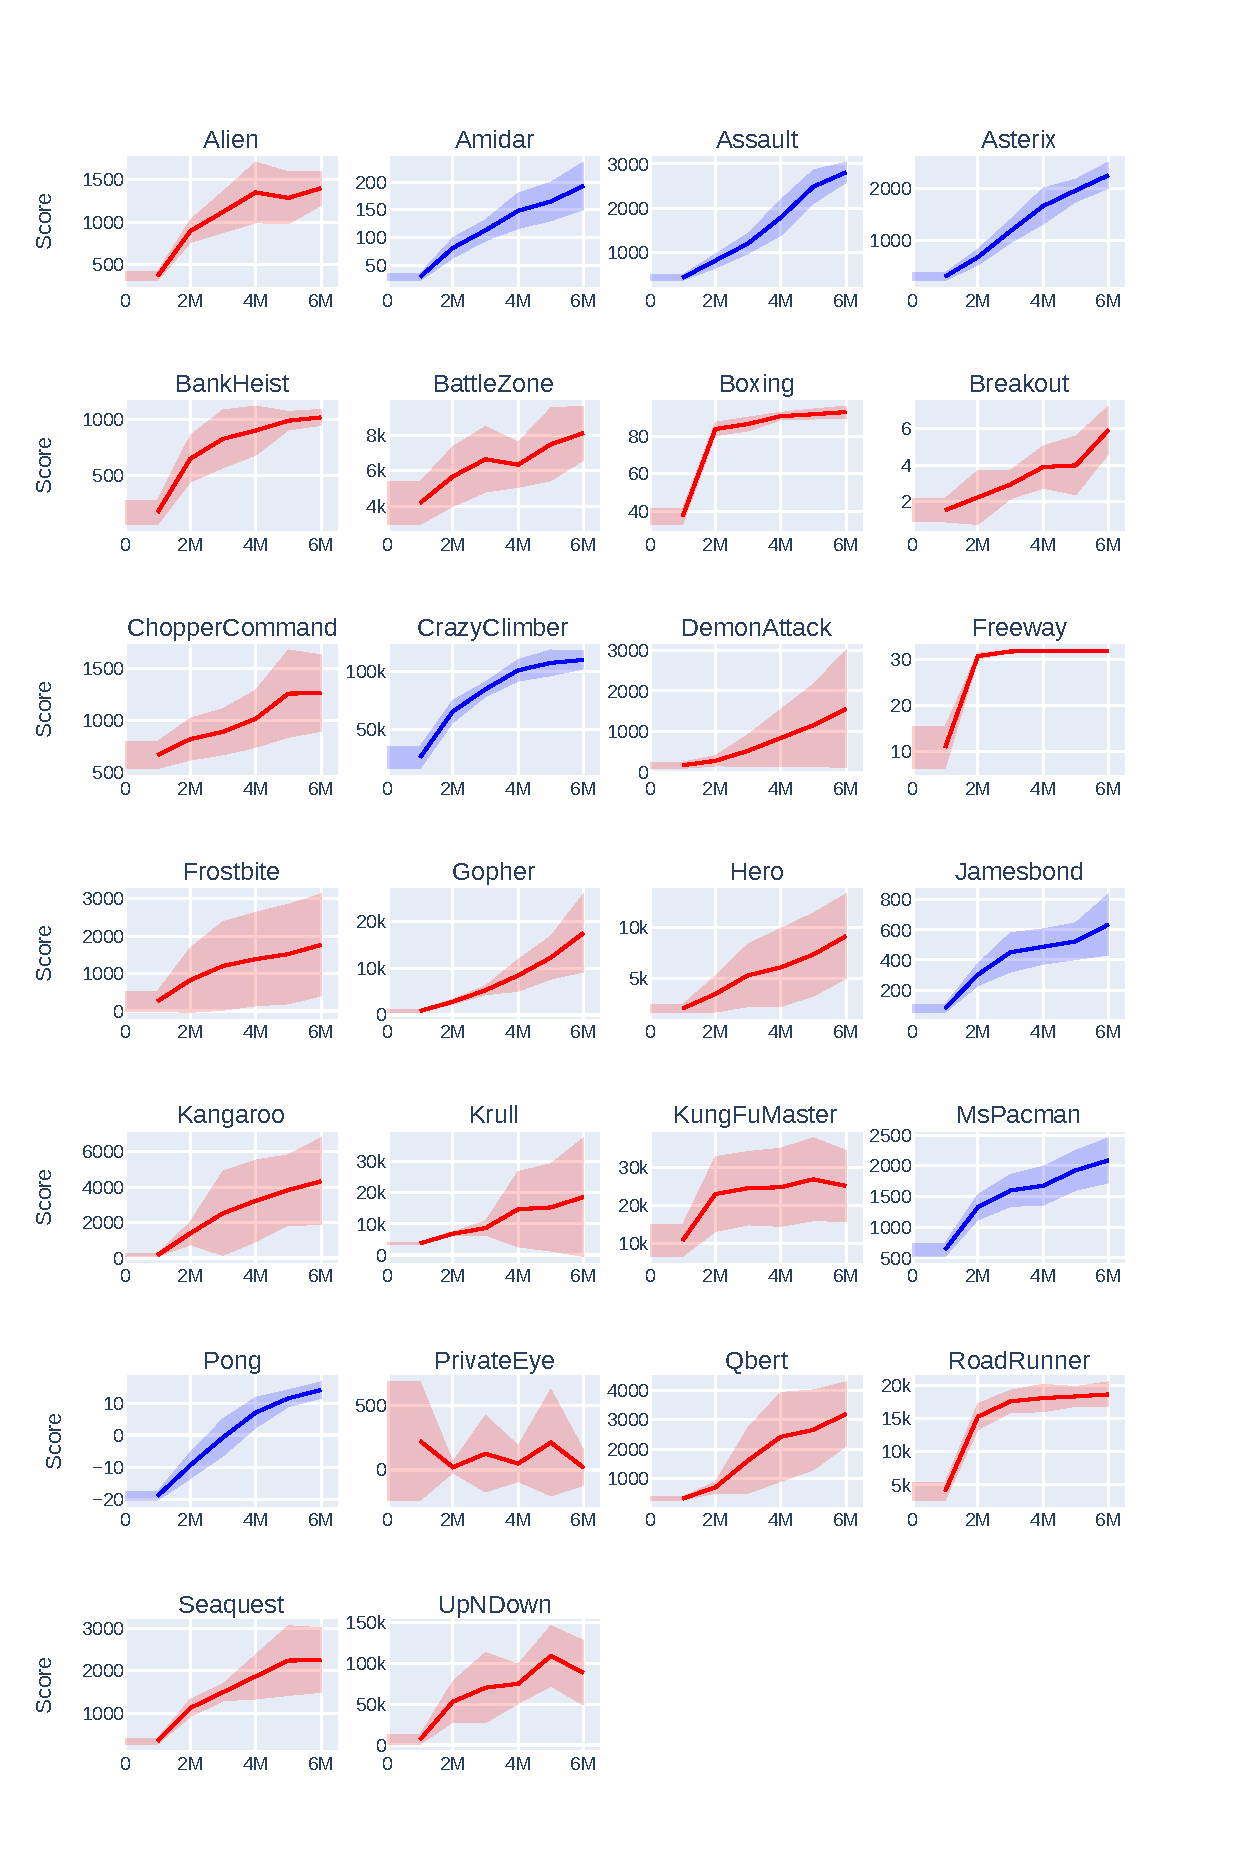
\includegraphics[width=\figurewidth,height=0.6\paperheight,keepaspectratio]{assets/env_selection.pdf}
  \caption{Performance curves for Atari games, with default settings and a time limit of $6 \times 10^6$. The values have been provided by the authors of the DreamerV2 paper. The x-axis represents the number of environment steps passed. The y-axis represents the validation score. Blue curves indicate environments, which we have selected for further evaluation.}
  \label{fig:atari_100k_comp}
\end{figure}

Next, we select out of this subset 3 games, which are most predictive of the performance on the complete 26-game benchmark. We follow the approach of \autocite{aitchisonAtari5DistillingArcade2022} and use the source code provided by the authors to arrive at the final result. The three environments selected by the algorithm are: \env{Assault}, \env{CrazyClimber} and \env{MsPacman}.

We use the same environment settings (frame skip values, time limit etc.) as the original DreamerV2 agent.

Since the original implementation of DreamerV2 is written in Tensorflow, we have ported the relevant source code (mainly the implementation of the world model and the actor critic) to Pytorch, resulting in slight changes in overall performance. It remains, however, comparable: \autoref{fig:torch_v_ref} depicts the validation score curves for both the original implementation, and the Pytorch version.

\begin{figure}
  \centering
  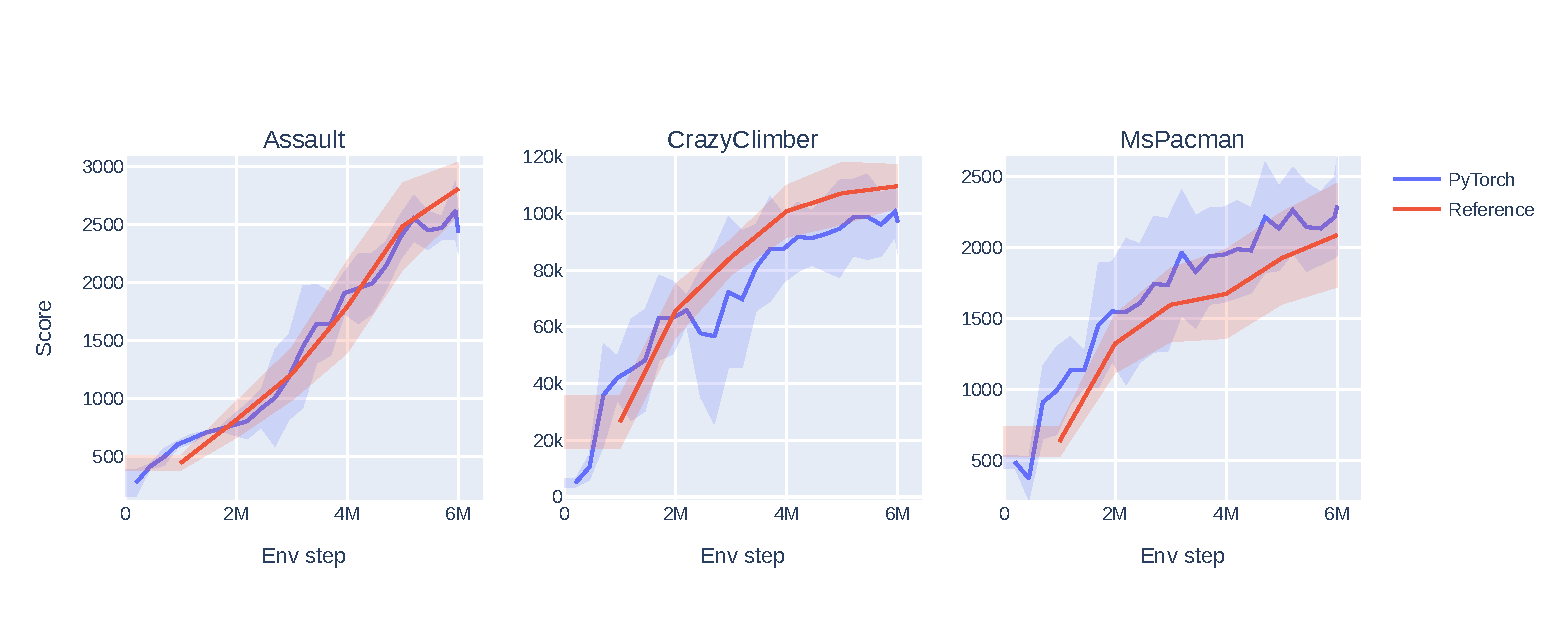
\includegraphics[width=\figurewidth,height=\paperheight,keepaspectratio]{assets/torch_v_ref.pdf}
  \caption{Comparison of the validation scores for Tensorflow and Pytorch versions. \emph{Note:} The scores for the reference (Tensorflow) version have been supplied by the authors, and were not verified independently.}
  \label{fig:torch_v_ref}
\end{figure}

\subsection{Evaluation protocols in Atari-100k benchmark}

A significant part of the setup is the agent evaluation protocol. To date, there is no standardized way to assess agent's performance in Atari-100k benchmark. Of the recent state-of-the-art architectures, DreamerV3 does not appear to use any post-training evaluation episodes, BBF and SimPLe do not specify the evaluation setup used, and IRIS, along with SR-SPR, use 100 evaluation trajectories, following \autocite{agarwalDeepReinforcementLearning2022}. Because we also measure validation performance throughout training, to avoid excessive impact of performing evaluation on training time, we choose the number of 32 evaluation episodes for measuring agent's performance.

\section{Training recipe optimization}

In the first order, we will investigate the training recipe-level optimizations, specifically tuning the data-to-update ratio. The rationale is to find the optimal update-to-data regime, and to establish a baseline for further analysis.

\subsection{Simple speedup test}
\label{sec:baseline}

We begin with an experiment involving a straightforward increase of the frequency of optimization steps, without any further changes.

\paragraph{Setup} Base DreamerV2 training recipe (\autoref{alg:dreamerv2_loop}) begins with a prefill of $P = 200 \times 10^3$ and continues until the total step count is $T = 200 \times 10^6$. The latter loop consists of $K = 64$ env steps (at the frame skip value of $4$, this corresponds to $16$ agent steps) and a single optimization step, consisting of optimizing the world model, and using the obtained model states to optimize the RL module.

\begin{algorithm}
  \caption{Base DreamerV2 training loop}
  \label{alg:dreamerv2_loop}
  \begin{algorithmic}[1]
    \State Gather $P$ env samples with an agent acting randomly, and put them into a replay buffer
    \While{Total number of env steps $<T$}
    \State Optimize the world model using batch of real rollouts $\left\{(o_{1:L}, a_{1:L-1}, r_{1:L-1}, \gamma)_i\right\}_{i=1}^N$ drawn from the replay buffer.
    \State Optimize the RL agent using the batch of dream data $\left\{(s_{1:H}, a_{1:H-1}, \widetilde{r}_{1:H-1}, \widetilde{\gamma}_{1:H})_i\right\}_{i=1}^{NL}$, generated by starting from the states obtained through an inference process on real-world rollouts, and imagining next $H-1$ states with the world model.
    \State Perform $K$ environment steps using the behavior policy, and store them in the replay buffer.
    \EndWhile
  \end{algorithmic}
\end{algorithm}

We replace $T$ by $400 \times 10^3$ to match Atari-100k benchmark environment budget, and $P$ with $20 \times 10^3$. Then, we perform tests with varying values of $E \in \{64, 32, 16, 8, 4, 2\}$, for a set of $3$ selected environments and $5$ RNG seeds.

Beyond that, for testing purposes, we also add an online train-validation split mechanism: each episode in the replay buffer is assigned either to the training set or the validation set -- to be precise, every $(1/p)$-th episode, starting from the first one, is assigned to the validation set, where $p = 0.15$. As a side-effect, we optionally extend the buffer prefill stage until at least one training and one validation episode have been collected.

\paragraph{Results} Let us first analyze final test performance, depending on the data-to-update ratio $K$, for each environment (\autoref{fig:baseline_score}). The mean final score is maximized for a given region of the values of $K$, beyond which it decreases, presumably either due to under- or overoptimization. Notably, for each task, the optimal value is different: $2-4$ for \env{CrazyClimber}, $\approx 8$ for \env{Assault} and a wide range for \env{MsPacman}.

\paragraph{Conclusions} Update frequency tuning yields substantial performance increases. The optimal value should be tuned, preferably for each environment separately.

\begin{figure}
  \centering
  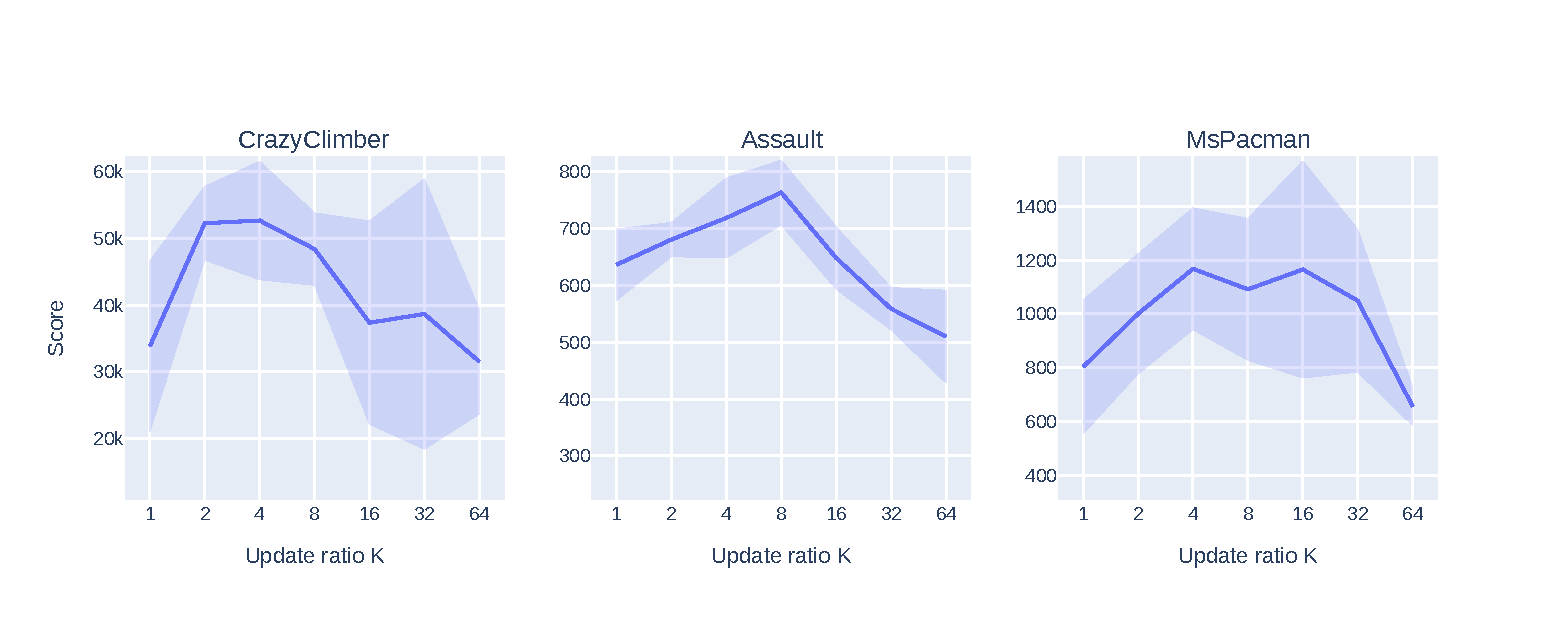
\includegraphics[width=\figurewidth,height=\figureheight,keepaspectratio]{assets/baseline_score.pdf}
  \caption{Final test episode returns for each of the 3 tested environments, relative to the data-to-update ratio $K$. The line indicates the mean across the RNG seeds, and the shaded area indicates the standard deviation. \emph{Note}: The x-axis is logarithmic.}
  \label{fig:baseline_score}
\end{figure}

\subsection{Decoupling model and RL optimization}
\label{ssec:decoupled_ratio}

The optimal training schedules for the model and the RL module need not coincide - we may, for example, find that the model is overfitting, yet the RL head remains underoptimized. The next experiment aims to investigate the empirical effects of decoupling model and RL update frequencies.

\paragraph{Setup} We adjust the code, relative to \autoref{sec:baseline}, so that the model is optimized once every $K_{\rm WM}$ environment steps, and the RL module is optimized once every $K_{\rm RL}$ environment steps. A grid search is performed for \env{Assault} environment alone, due to computational constraints, with ratios $K_{\rm WM}, K_{\rm RL} \in \{2, 4, 8\}$, corresponding to the observed regime, where the performance starts decreasing.

\paragraph{Results} \autoref{fig:split_ratios_perf} displays the agent performance depending on the configuration of the ratios. Both the model and the RL ratios play a significant role in determining the final score, though no clear pattern can be determined - for example, increasing the RL update ratio does not necessarily improve the performance, as the score for $K_{\rm WM} = 4, K_{\rm RL} = 2$ is lower than the score for $K_{\rm WM} = 4, K_{\rm RL} = 4$.

\paragraph{Conclusions} RL and model update ratios should be decoupled and tuned separately.

\begin{figure}
  \centering
  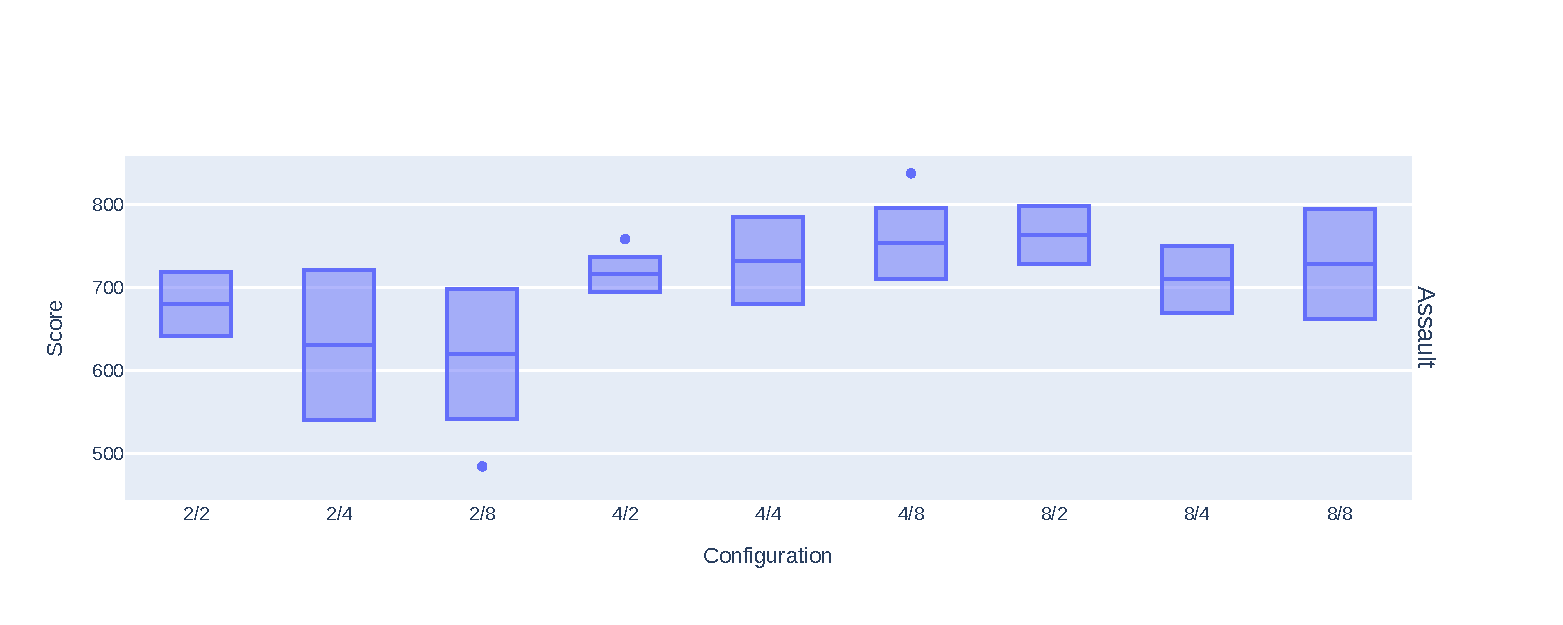
\includegraphics[width=\figurewidth,height=\figureheight,keepaspectratio]{assets/split_ratios_perf.pdf}
  \caption{Final validation score for each model/RL update ratio configuration. The x-axis represents each run, marked by a tag in the form of '$K_{\rm WM}/K_{\rm RL}$'. The points represent the scores for each seed, with the corresponding box plot to the right.}
  \label{fig:split_ratios_perf}
\end{figure}

\section{Investigating the learning dynamics of the agents}

So far, the experiments suggest that achieving optimal or near-optimal performance may require, at the very least, a hyperparameter sweep over \emph{both} model and RL update frequencies. Given the increase in the number of training runs this would require, we are in dire need of an auto-selection schema for these parameters. In order to achieve this, we will start with an examination of the various metrics thoughout the run, and see whether they are correlated with the final score. The idea is that, if we are able to detect signs of applying non-optimal training schedules, e.g. through under- or overfitting, we might be able to adjust these parameters to reach the optimal regimes automatically and achieve maximal final performance.

\subsection{Analyzing the world model}
\label{ssec:wm_analysis}

\subsubsection{Model validation loss}

Since model learning is a supervised learning task, the clearest indicator of under- or overfitting ought to be the validation loss. We compute it as follows: throughout the training process (to be precise, every $16$ model optimization steps), we load a batch of data using the validation episodes only, and compute the mean model loss for these items.

\paragraph{Results} We will start with the aggregate results - the relationship between the final validation loss and the final agent performance, for the equal-ratio experiment described in \autoref{sec:baseline}. As we can see in \autoref{fig:val_v_perf}, it would appear, somewhat surprisingly, that the value, for individual training runs, is not meaningfully correlated with the final score achieved by the agent. We can also see, that the agents do not, in general, exhibit classical overfitting behavior, in the sense that the validation loss curves plateau at worst, and in general the loss value keeps decreasing. The learning process nevertheless degrades, as the final values of the validation loss keep increasing as the ratio of the optimization and environment steps increases. The ratio values, for which the final loss value is the smallest, do not correspond to the ones which achieve the highest performance.

\paragraph{Conclusions} The relationship between the model validation loss and the agent performance is nontrivial.

\begin{figure}
  \centering
  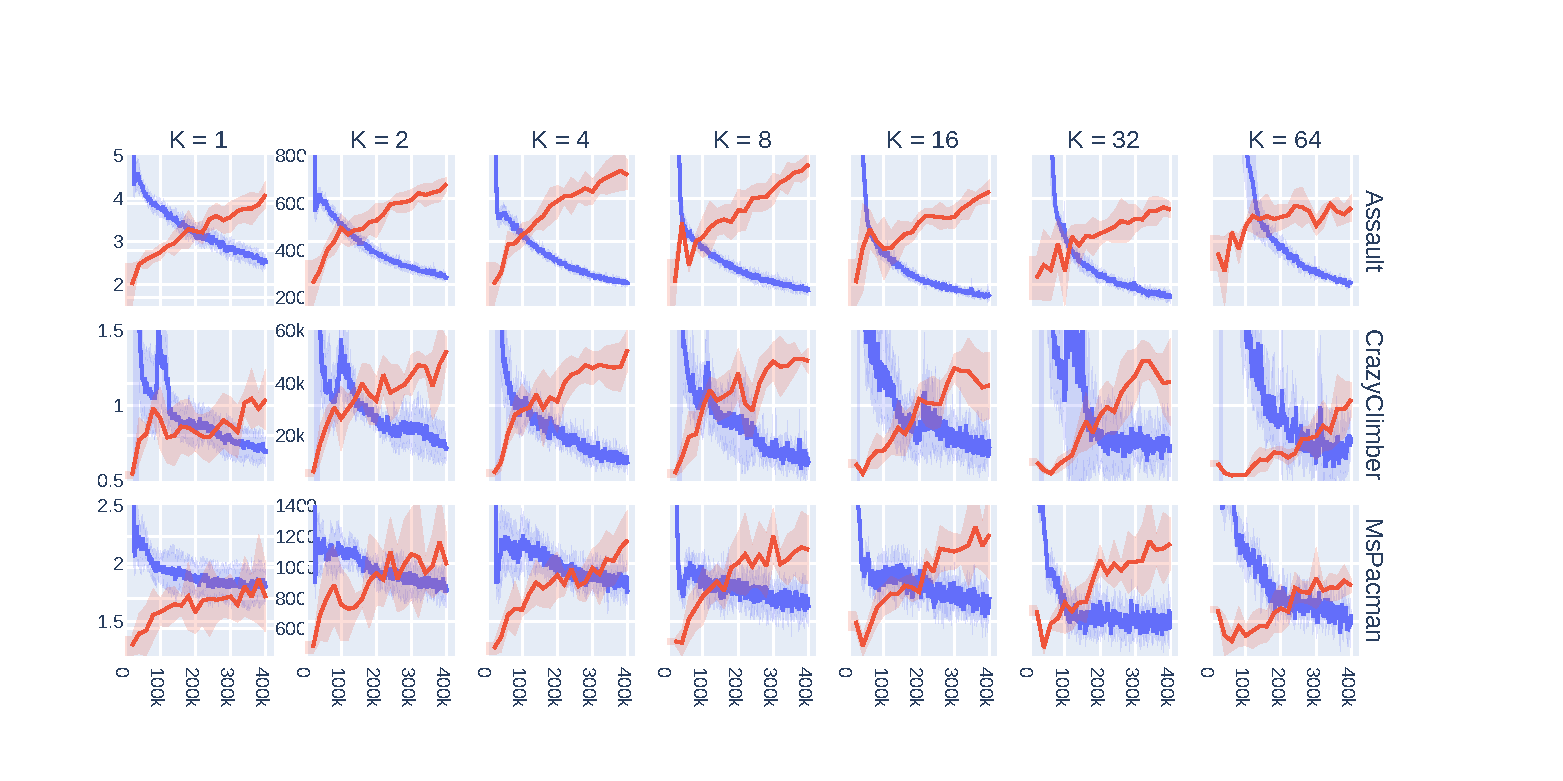
\includegraphics[width=\figurewidth,height=\figureheight,keepaspectratio]{assets/val_loss_v_perf.pdf}
  \caption{Relationship between model validation loss and validation score curves. Each row represents a different Atari game, and each columns a different model/RL update ratio used. On each subplot, curves of two metrics are displayed: model validation loss (decreasing) and validation scores (increasing), averaged over 5 RNG seeds.}
  \label{fig:val_v_perf}
\end{figure}

\subsubsection{Model training loss}

To further examine the behavior of the agent throughout the optimization process, let us take a look at the \emph{training} loss curves (\autoref{fig:train_v_perf}). We can see a clear monotonic relationship between the final loss value achieved and the update frequency, though, as before, the better values do not lead to improvements in terms of the quality of the agents. Perhaps more interestingly, at very high update frequencies (i.e. small data-to-update ratios), the optimization process seems to stall out completely. For the value of $K = 1$, for example, in all three environments tested, near-``optimal'' value is reached after the first $100 \times 10^3$ environment steps, whereafter it either improves marginally, or even increases.

\paragraph{Conclusions} The relationship between the model training loss and the agent performance is nontrivial as well.

\begin{figure}
  \centering
  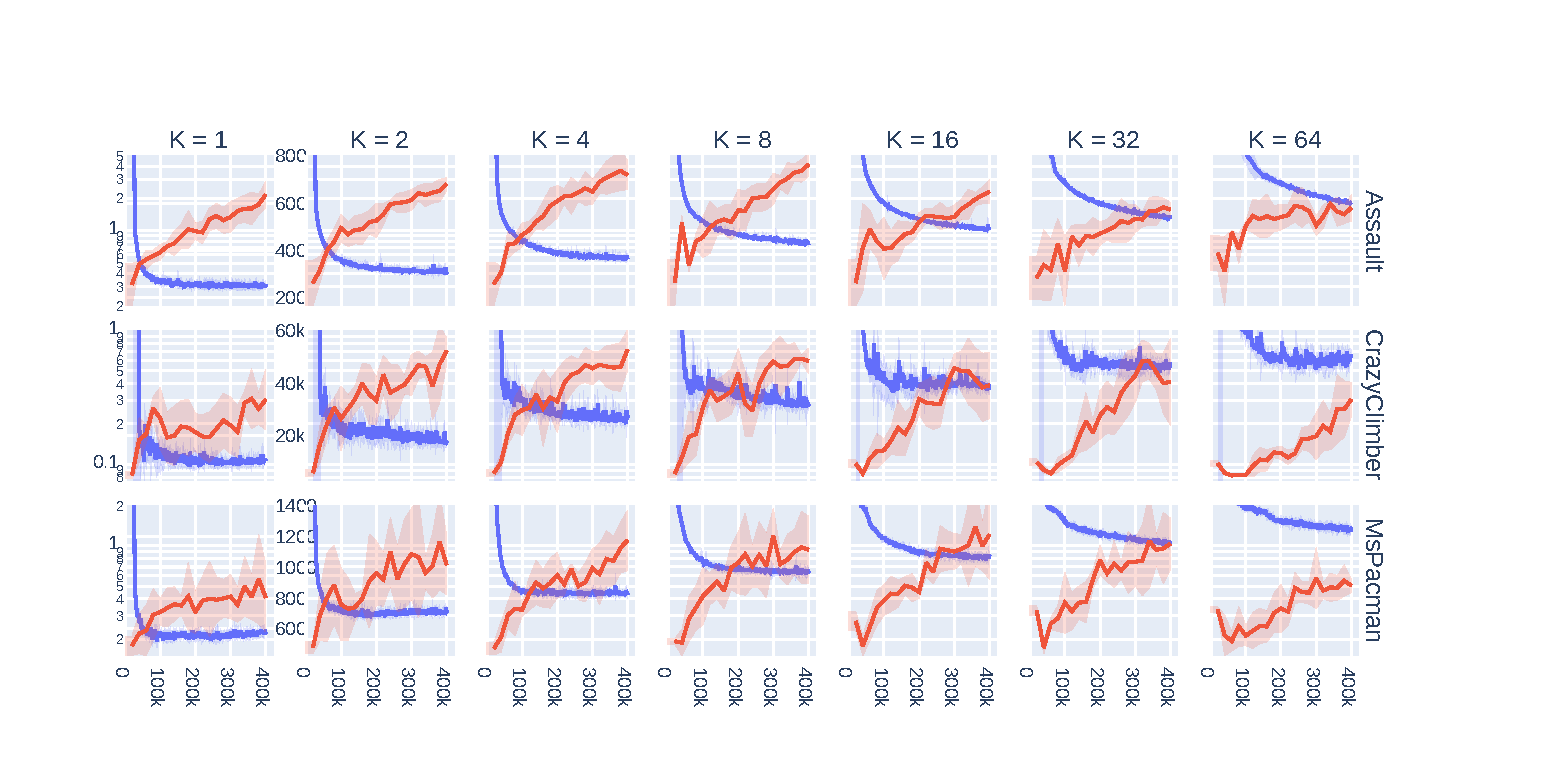
\includegraphics[width=\figurewidth,height=\figureheight,keepaspectratio]{assets/train_loss_v_perf.pdf}
  \caption{Relationship between model training loss and validation score curves. Each row represents a different Atari game, and each columns a different model/RL update ratio used. On each subplot, curves of two metrics are displayed: model training loss (decreasing) and validation scores (increasing), averaged over 5 RNG seeds.}
  \label{fig:train_v_perf}
\end{figure}

\section{Auto-tuning update frequencies}

The findings in \autoref{ssec:wm_analysis} suggest, that model validation loss cannot be directly used for the purposes of guiding the optimization process. There exist, however, works doing precisely that, which demands a further inquiry.

\paragraph{Setup} We will specifically perform a closer examination of \autocite{dorkaDynamicUpdatetoDataRatio2023}. The approach taken by the authors is to check validation loss throughout the training process, and to decrease the update frequency if the loss value has degraded, and increase it if it has improved. To start off, we will replicate the experiment, albeit with some notable changes:

\begin{enumerate}
  \item The authors propose using image reconstruction loss as the validation metric. We would rather have the method apply to models other than DreamerV2's specifically, however, so will use the total loss value.
  \item A validation set is constructed differently: $3 \times 10^3$ transitions are collected every $100 \times 10^3$ steps, which corresponds to the flat $12 \%$ of the transitions being reserved for the validation set, whereas we reserve $15 \%$ of the \emph{episodes} instead. Thus, the training set contains transitions which immediately precede or succeed the ones in the validation set - whether it represents a form of data contamination is unclear.
\end{enumerate}

\paragraph{Results} The validation scores can be found in \autoref{fig:adaptive_v1_0}, along with the baseline results (\autoref{sec:baseline}) for the sake of comparsion. It would appear that the strategy is, in general, effective, though not universal - for example, the scores on \env{Assault} do not quite reach the performance peak.

\begin{figure}
  \centering
  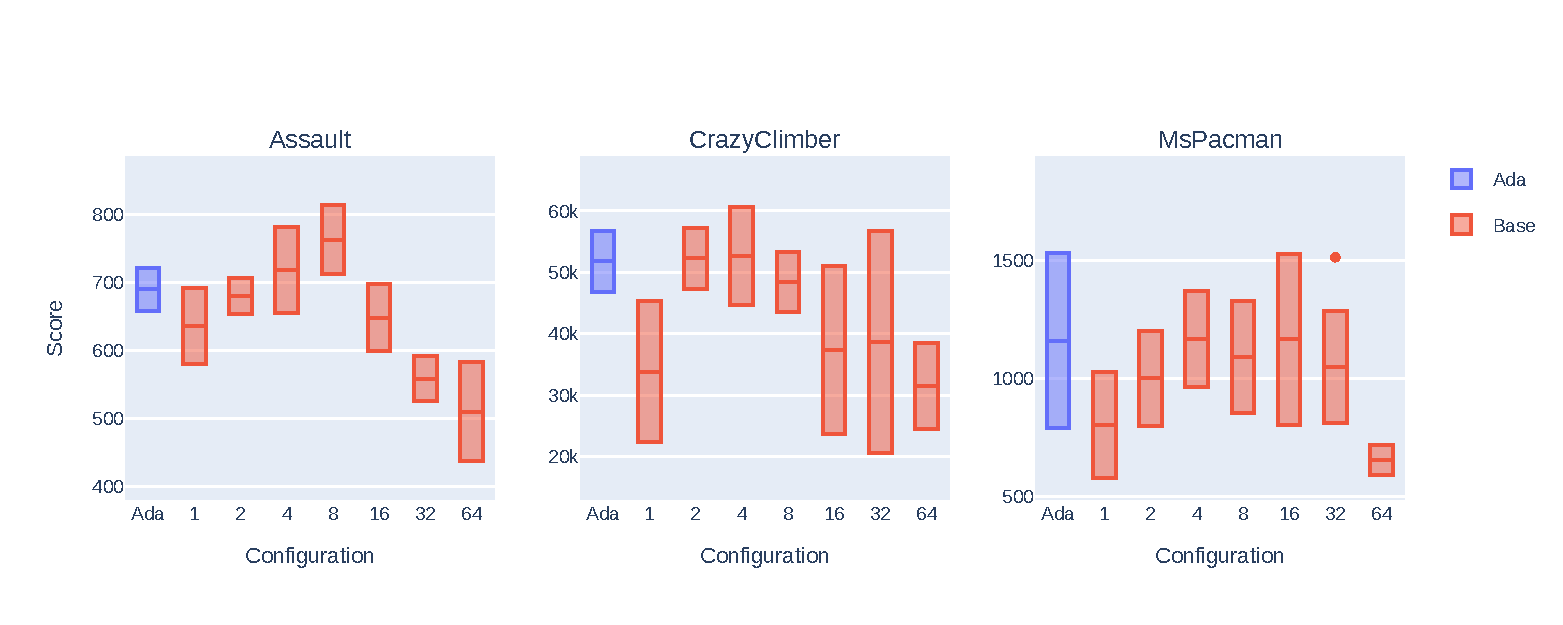
\includegraphics[width=\figurewidth,height=\figureheight,keepaspectratio]{assets/adaptive_v1_0.pdf}
  \caption{The comparison of the final validation scores, for the adaptive ratio experiment {\sf Ada} and the baseline experiments {\sf 1} - {\sf 64}, where the number denotes the model/RL update ratio $K$. Each subplot shows the results for a different environment tested. The bars signify mean and one standard deviation, obtained from a sample of $5$ training runs for each configuration.}
  \label{fig:adaptive_v1_0}
\end{figure}

Given that the idea behind this approach is to minimize model overfitting by monitoring validation loss, our next step is to look at the validation loss. The results (\autoref{fig:adaptive_v1_0_loss}) do not seem to imply that the method has a consistent positive effect on the model validation loss. In fact, if we compare validation loss curves and the current ratio values (\autoref{fig:adaptive_v1_0_curves}), the relationship is not precisely what we would expect. As noted previously, the idea behind the method is to increase update ratio as long as the validation loss decreases, and vice versa. In short time scales, specifically the $2 \times 10^3$ environment steps between each ratio update, this does occur, but across longer time spans, the coupling breaks. For example, for \env{MsPacman} and the RNG seed of $1$, the validation loss decreases up until the timestep of $200 \times 10^3$, yet the ratio keeps increasing. After the jump, presumably due to the influence of a new validation episode in the buffer, the loss value starts decreasing, and the ratio decreases.

\begin{figure}
  \centering
  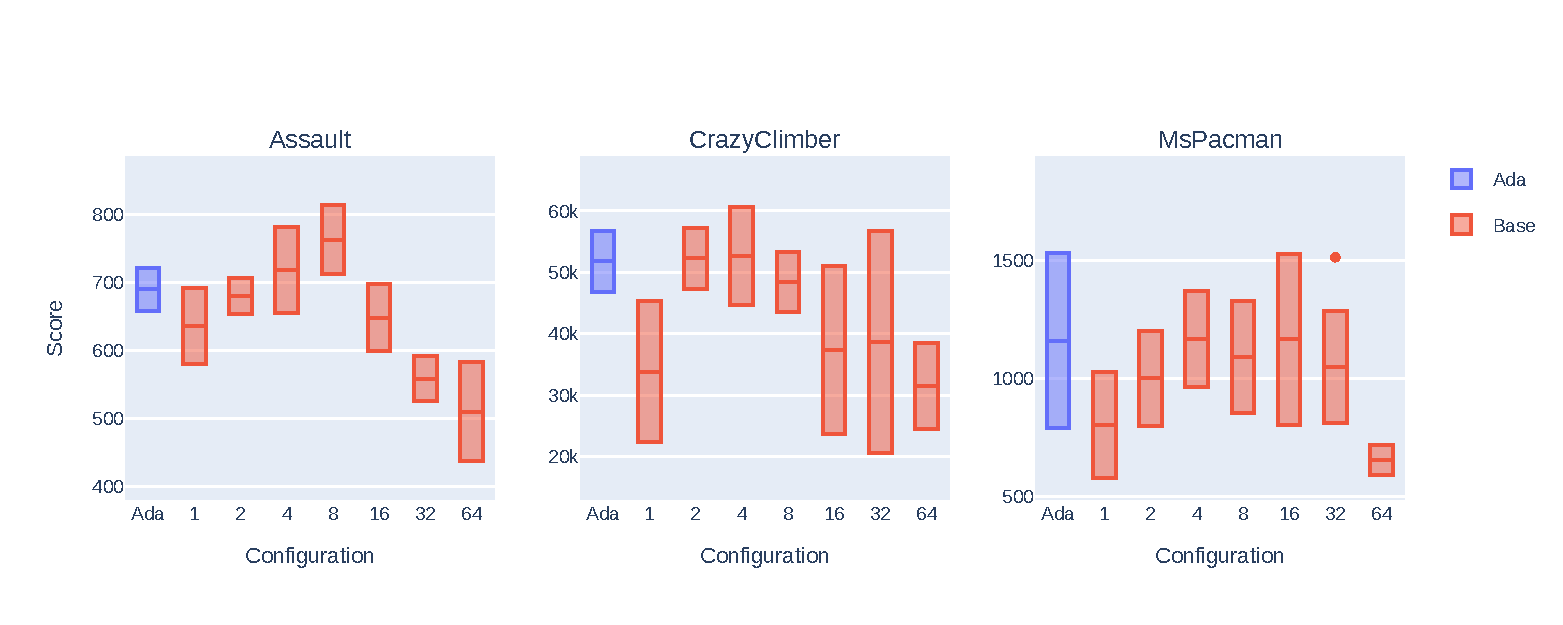
\includegraphics[width=\figurewidth,height=\figureheight,keepaspectratio]{assets/adaptive_v1_0.val_loss.pdf}
  \caption{The comparison of the final model validation loss values, for the adaptive ratio experiment {\sf Ada} and the baseline experiments {\sf 1} - {\sf 64}, where the number denotes the model/RL update ratio $K$. Each subplot shows the results for a different environment tested. The bars signify mean and one standard deviation, obtained from a sample of $5$ training runs for each configuration.}
  \label{fig:adaptive_v1_0_loss}
\end{figure}

\begin{figure}
  \centering
  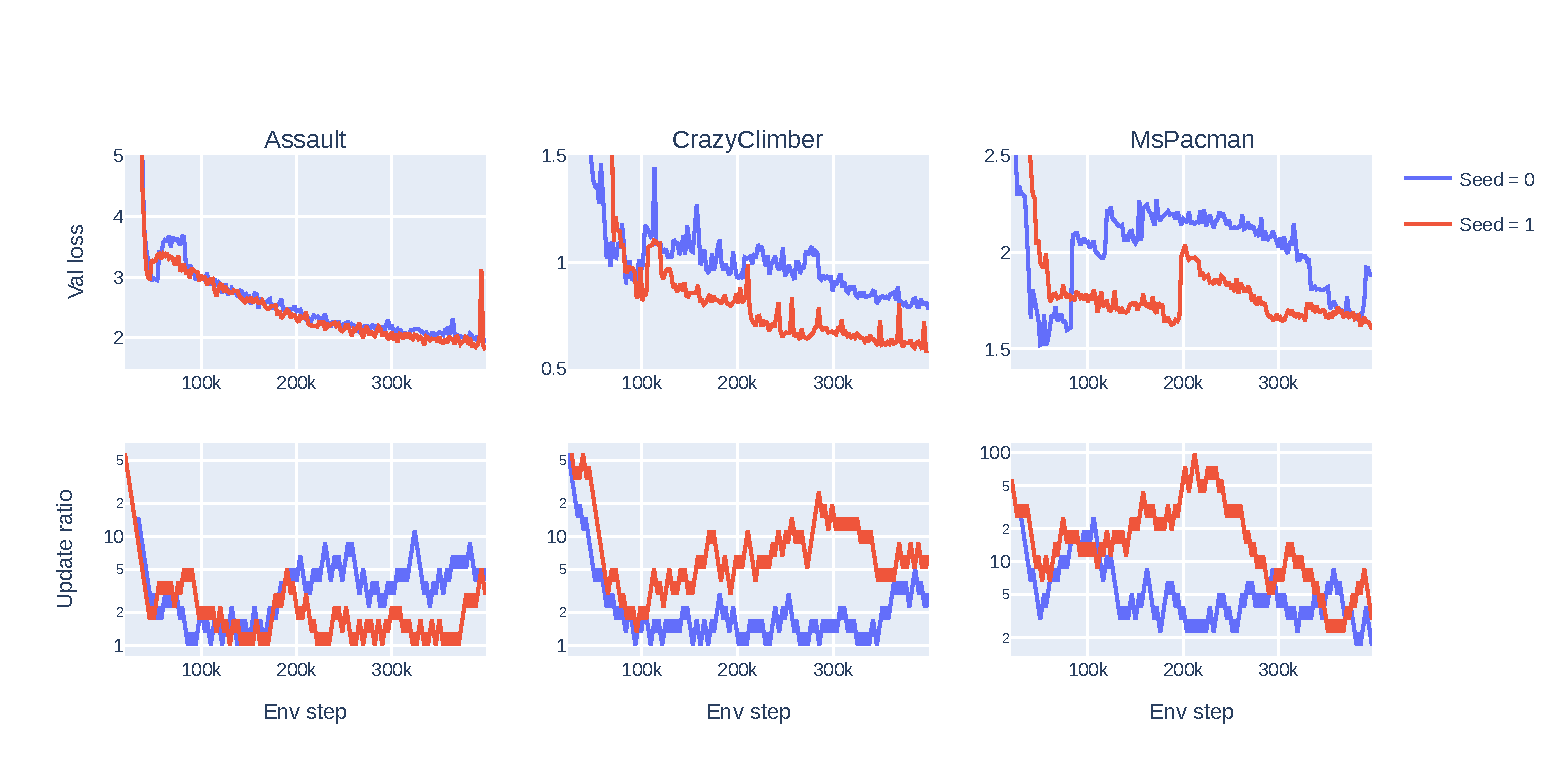
\includegraphics[width=\figurewidth,height=\figureheight,keepaspectratio]{assets/adaptive_v1_0.curves.pdf}
  \caption{The curves for the model validation loss and the current update ratio, for the adaptive ratio experiment. Each column represents a different Atari task. Two training runs, corresponding to two different RNG seeds, are shown on each subplot. The model validation curves have been smoothed with exponential moving average to improve the clarity of the presentation.}
  \label{fig:adaptive_v1_0_curves}
\end{figure}

\paragraph{Conclusions} It appears, that the theoretical underpinnings behind the effectiveness of this approach are not quite as clear as one would hope. Unfortunately the source paper \autocite{dorkaDynamicUpdatetoDataRatio2023} does not supply any concrete analysis of the validation loss itself - only the agent performance and update ratio curves are provided - meaning it is impossible to ascertain whether the observations are an artifact of different experimental setup.

\subsection{Decoupled adaptive ratio system}

Irrespective of the theoretical basis, the method of adapting update ratios has proven provisionally effective. We believe one further improve upon this method. Drawing on the results concerning the decoupling of the optimization rates for the model and the RL modules, we propose a similar decoupling in the adaptive regime. In particular, we will make only the model update ratio adaptive, and keep the RL update ratio fixed at a pre-defined value. Although an automatic method to select the RL update frequency would be welcome, we consider it out-of-scope for this thesis due to inherent complexity of the undertaking, arising from the nontrivial RL algorithm dynamics coupled with equally complex interaction between the model itself and the RL component.

\paragraph{Results} The results (\autoref{fig:adaptive_wm_v1_0}) indicate, that the decoupling has an overall positive impact on the agent performance, consistent with the findings in \autoref{ssec:decoupled_ratio}. However, it must be noted, that the benefit depends on the environment in question, and the value of the RL update ratio $K_{\rm RL}$. For example, for the value of $K_{\rm RL} = 8$, the agent exhibits degraded performance relative to the coupled-ratio setting, making it a sensitive hyperparameter needing to be tuned.

\paragraph{Conclusions} Decoupling the RL update ratio in the adaptive ratio system can yield further performance improvements.

\begin{figure}
  \centering
  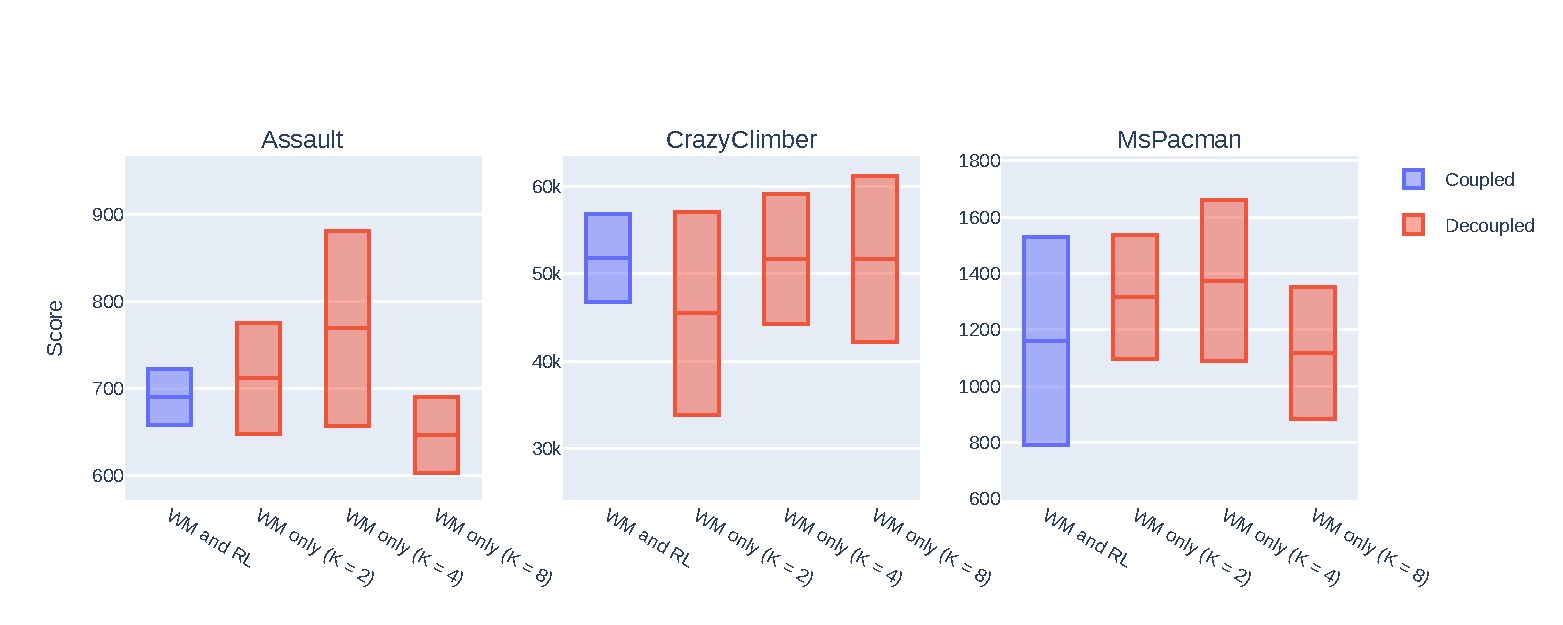
\includegraphics[width=\figurewidth,height=\figureheight,keepaspectratio]{assets/adaptive_wm_v1_0.pdf}
  \caption{A comparison between the final validation scores for the coupled and the decoupled variants of the adaptive update ratio experiment. Each subplot represents a different environment tested. Each box signifies the results for a given configuration - mean and one standard deviation, obtained from a sample of $5$ training runs for each configuration.}
  \label{fig:adaptive_wm_v1_0}
\end{figure}

\section{Data augmentation}

Incorporating data augmentation into an RL framework can be done in non-trivial ways. DrQ, for example, combines transforming the input, averaging the $Q$ functions across multiple augmented samples, and averaging the $Q$ targets. In the context of model-based RL, one could develop similar schemes for both the world model and the RL modules, e.g. by averaging posterior state distributions over multiple image augmentations. This, however, would require changing the implementation of these modules, whereas our goal is to make the framework as modular as possible. Therefore, we opt to only augment the input, and forego the averaging of various quantities in question.

\subsection{Random shifts test}
\label{ssec:random_shift}

\paragraph{Setup} We follow the original paper in choosing random shifts (of maximum value of $4$ pixels) as the image transformation to apply. The augmentations will be applied to both images in the batch for the model optimization, and the batch used to generate the initial states for the imagined rollouts. As far as the training recipe is concerned, we will start with a fixed-ratio setup (\autoref{sec:baseline}) in order to compare the data-augmented recipe with a non-data-augmented baseline. We perform the test for two values of model/RL update ratio, $K = 2$ and $K = 4$.

\paragraph{Results} The comparison of the test episode returns for the two variants (\autoref{fig:data_aug}) shows, that, with the base settings, the addition of data augmentation \emph{degrades} performance, excepting perhaps \env{MsPacman}. As the main idea behind data augmentation is the reduction of model overfitting, we will next investigate the training and the validation loss curves for the model. The analysis of the model validation loss curves for each variant (\autoref{fig:data_aug_val_curves}) reveals, that not only is it significantly higher compared to the baseline variant, but it also does not improve as the update frequency increases (equivalently, $K$ decreases). In general, though, the validation loss curves follow the same overall trajectory, making it hard to discern why performance degrades on, say, \env{CrazyClimber}, and not on \env{MsPacman}.

\begin{figure}
  \centering
  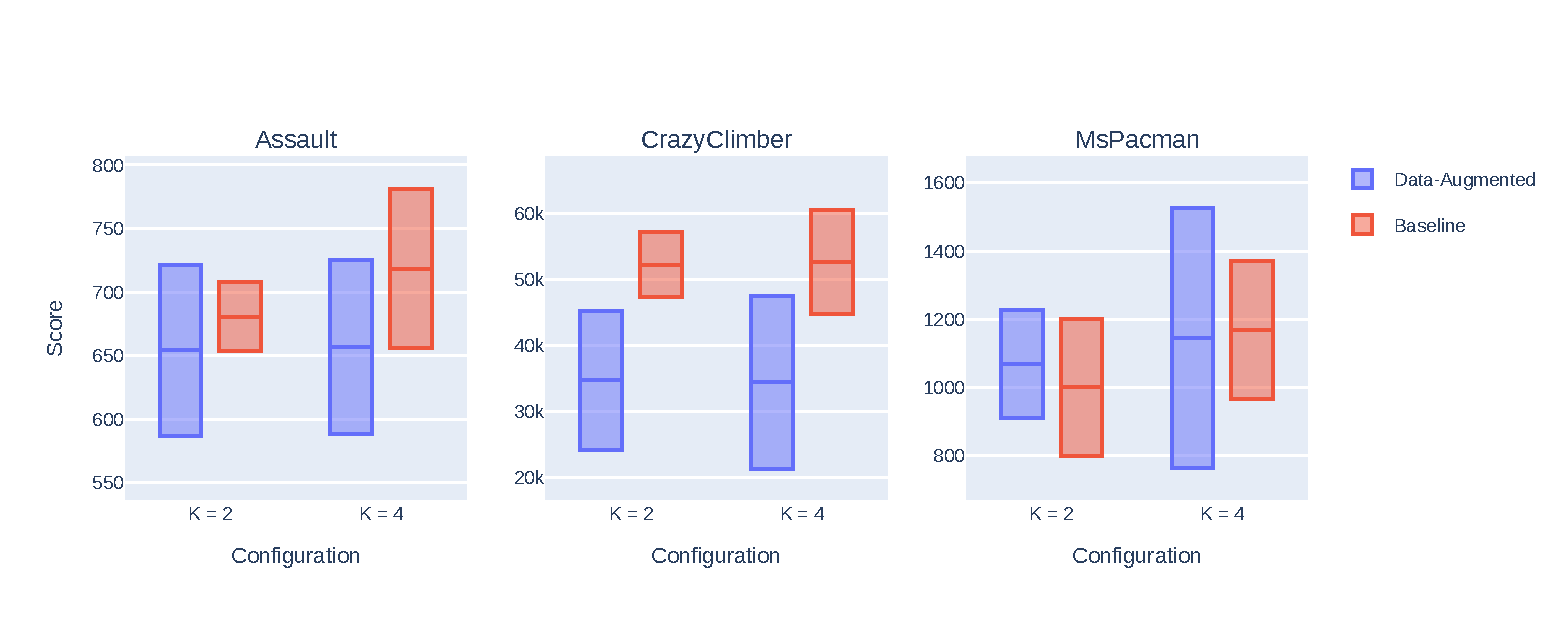
\includegraphics[width=\figurewidth,height=\figureheight,keepaspectratio]{assets/data_aug.pdf}
  \caption{A comparison of the final validation scores for the data-augmented agent, and a non-data-augmented baseline. Each subplot represents the results for a single environment. In each subplot, results for different values of model/RL update ratio $K$ are grouped together. Each group contains a box, signifying the mean and the standard deviation evaluated across $5$ training runs, for the data-augmented and the non-data-augmented variants.}
  \label{fig:data_aug}
\end{figure}

\begin{figure}
  \centering
  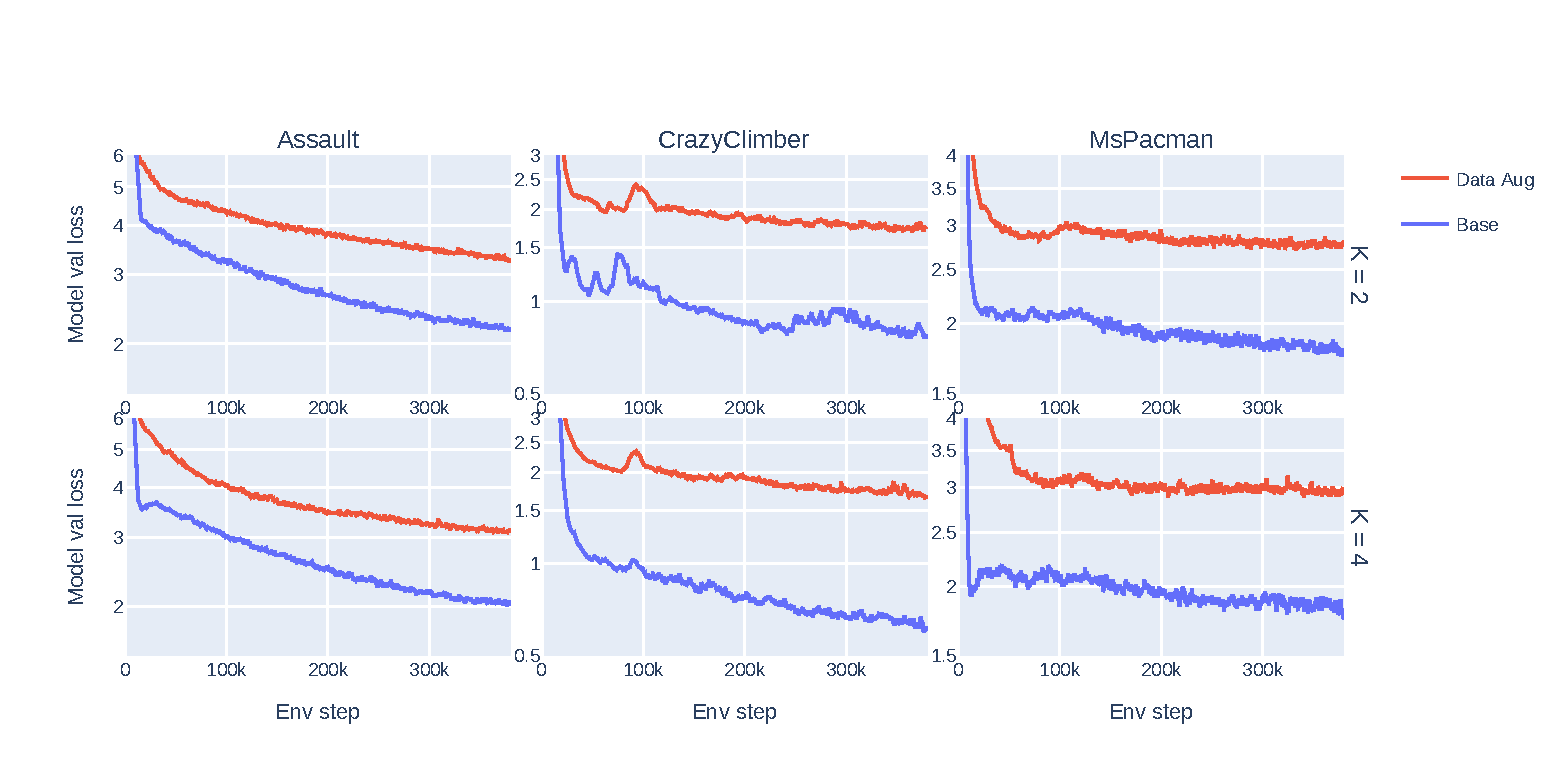
\includegraphics[width=\figurewidth,height=\figureheight,keepaspectratio]{assets/data_aug.val_curves.pdf}
  \caption{A comparison of the model validation loss curves for the data-augmented agent, and a non-data-augmented baseline. Each column represents the results for a single environment. Each row corresponds to a different configuration - model/RL update ratio used. In each subplot, curves for the data-augmented and non-data-augmented variants are displayed. The curves have been smoothed by exponential moving average, to improve the clarity of the presentation.}
  \label{fig:data_aug_val_curves}
\end{figure}

If we take a look at the model training loss curves (\autoref{fig:data_aug_train_curves}), we may observe a following phenomenon: for \env{Assault} and \env{CrazyClimber}, the addition of random shifts appears to slow down, or even stall out the training process, as shown by the slower rate of decrease (in log-space). For \env{MsPacman}, however, the reverse is true: in the original experiment, training loss stops improving at a certain point, whereas in the data-augmented scenario, we observe a consistent decrease. This may be indicative of data augmentation making the optimization process too difficult, rather than having it alleviate overfitting.

\begin{figure}
  \centering
  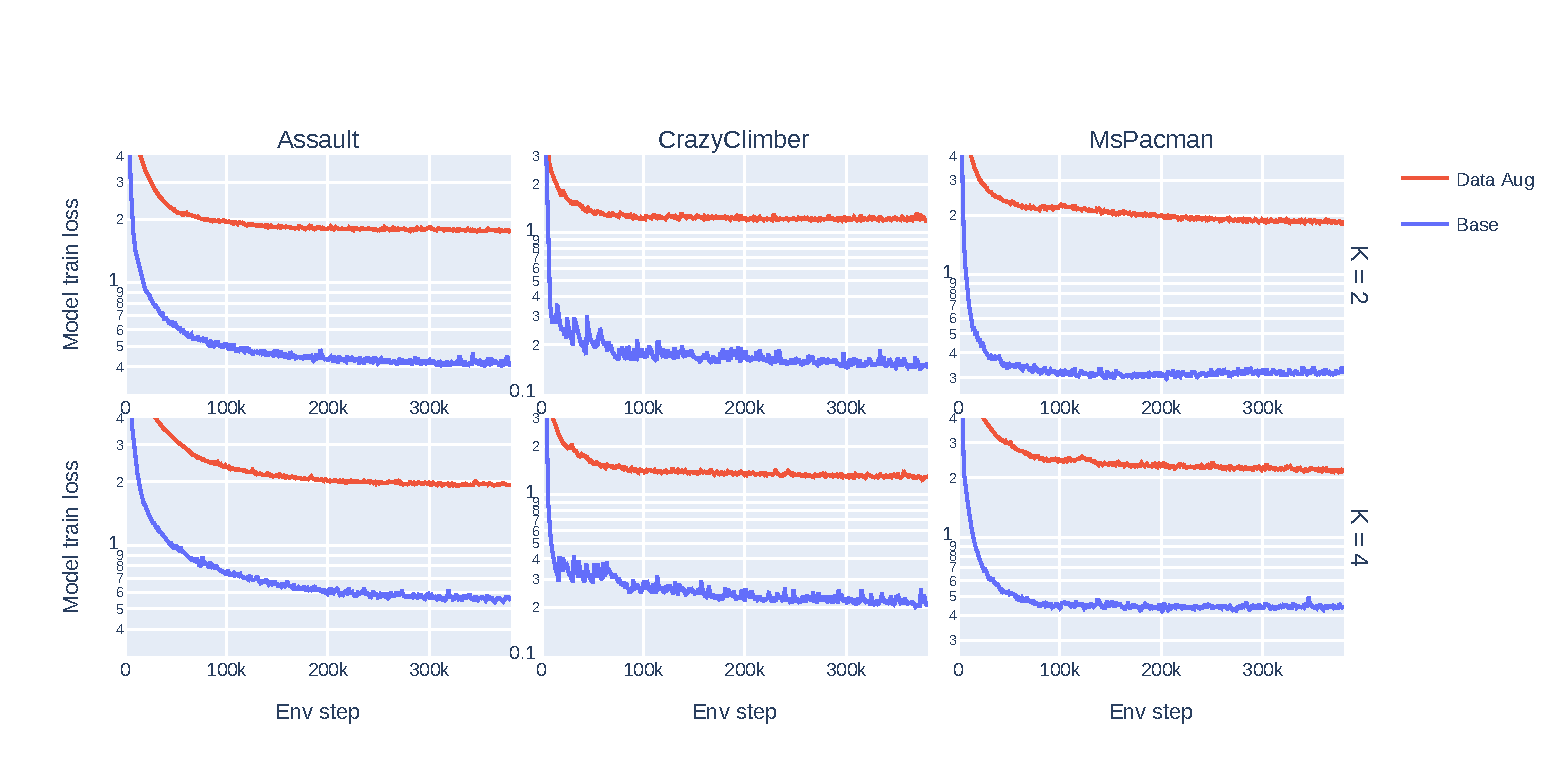
\includegraphics[width=\figurewidth,height=\figureheight,keepaspectratio]{assets/data_aug.train_curves.pdf}
  \caption{A comparison of the model training loss curves for the data-augmented agent, and a non-data-augmented baseline. Each column represents the results for a single environment. Each row corresponds to a different configuration - model/RL update ratio used. In each subplot, curves for the data-augmented and non-data-augmented variants are displayed. The curves have been smoothed by exponential moving average, to improve the clarity of the presentation.}
  \label{fig:data_aug_train_curves}
\end{figure}

\paragraph{Conclusions} Using the default data augmentation techniques does not have a positive effect on the agent performance, nor does it appear to help with model overfitting.

\subsection{Different image augmentation types}

As suggested in \autocite{kostrikovImageAugmentationAll2021}, the type of image augmentation used has a large impact on the effectiveness of the method. To this end, the next experiment will assess the impact of changing the kind of the augmentation.

\paragraph{Setup} We mostly follow the source paper in the selection of the transforms to test:

\begin{enumerate}
  \item {\tt none}: Baseline/No augmentations applied.
  \item {\tt shift4}: (Default) Apply a random image shift. The shift in each axis is selected randomly from $\{-4, \ldots, 4\}$.
  \item {\tt shift2}: Apply a random image shift. The shift in each axis is selected randomly from $\{-2, \ldots, 2\}$. This variant of {\tt shift4} is motivated by the fact, that DrQ image size is $84 \times 84$, whereas we operate on images of size $64 \times 64$ - it could be possible, that the shift of $4$ is too large.
  \item {\tt cutout}: Perform random erasing with probability $p = 0.5$.
  \item {\tt intensity}: Perform random brightness/intensity increase. To be specific, each pixel's value is multiplied by $f \sim \mathcal{U}[0.95, 1.05]$.
  \item {\tt rotate}: Rotate the image by $d \sim \mathcal{U}[-5, 5]$ degrees.
  \item {\tt vflip}: Flip the image vertically, with probability $p = 0.1$.
\end{enumerate}

where $x \sim \mathcal{U}[a, b]$ denotes a sample from the uniform distribution over $[a, b] \subset \mathbb{R}$. Other than the data augmentation type, we follow experimental setup in \autoref{ssec:random_shift}, except that we check the configuration with update ratio $K = 8$ due to the number of augmentations to test, and attendant number of training runs to perform.

\paragraph{Results} The analysis of the validation scores (\autoref{fig:data_aug_sweep}) suggests, that no type of image augmentation has a consistent positive effect on the agent performance.

\begin{figure}
  \centering
  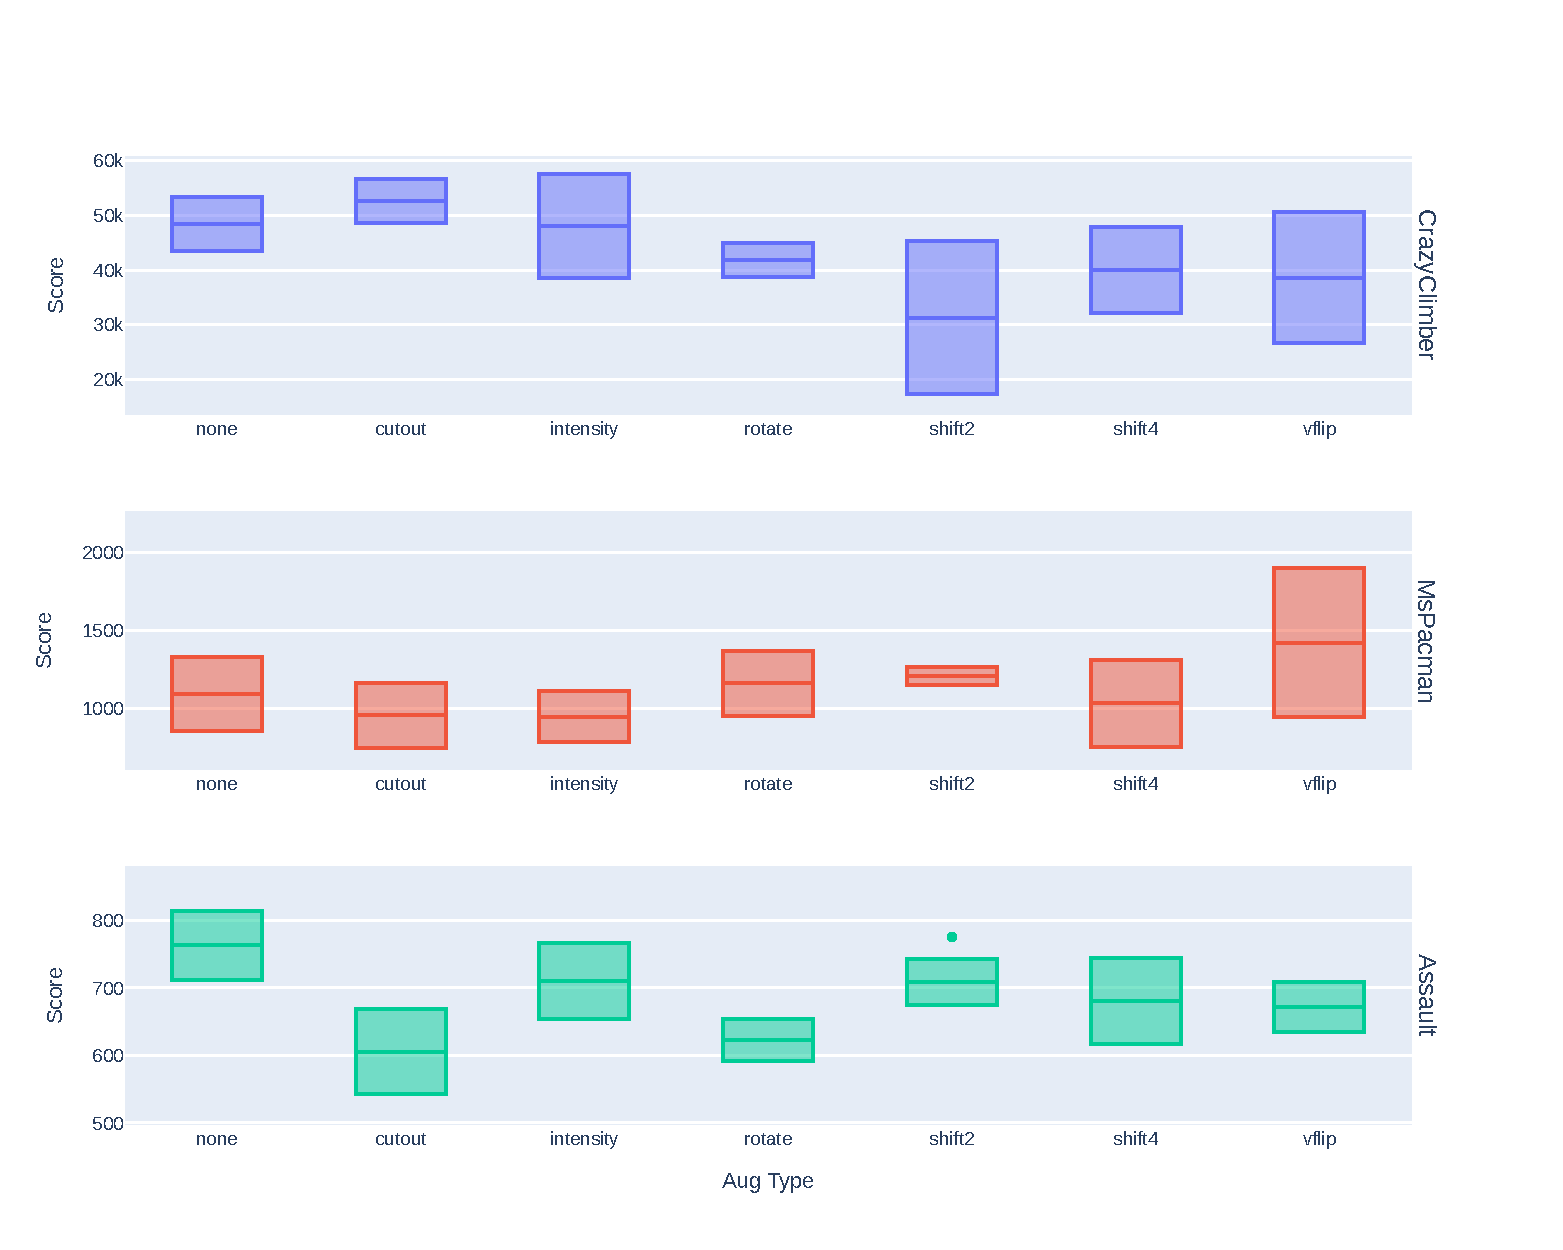
\includegraphics[width=\figurewidth,height=\figureheight,keepaspectratio]{assets/data_aug.sweep.pdf}
  \caption{The final validation scores for different data augmentation types. Each row contains the results for a different environment tested. Each of the boxes corresponds to a given augmentation type, and displays the mean and the standard deviation measured with a sample of $5$ training runs.}
  \label{fig:data_aug_sweep}
\end{figure}

\section{Choice of the RL algorithm choice}

So far, all the experiments have used the default RL module of DreamerV2, namely a variant of Advantage Actor-Critic (A2C). In this section, we shall investigate the effects of replacing it with Proximal Policy Optimization (PPO) and Soft Actor-Critic (SAC), whilst keeping the model component intact. Beyond hopefully achieving improvement in terms of agent performance, our objective is to elucidate the design choices when incorporating model-free RL algorithms into a model-based setting.

\subsection{Algorithmic details}

In order to be able to explain the design of the experiments, we need to briefly explain how SAC, PPO and CEM work. For detailed exposition of SAC and PPO, we refer the reader to \autocite{haarnojaSoftActorCriticOffPolicy2018} and \autocite{schulmanProximalPolicyOptimization2017} respectively.

\subsubsection{Soft Actor-Critic}

\begin{sloppypar}
  Soft Actor-Critic follows a maximum-entropy RL formulation, where the objective, the expected sum of rewards $J = \mathbb{E}\left[\sum_t r_t\right]$, is augmented with an entropy term $J' = \mathbb{E}\left[\sum_t \left\{r_t + \alpha \mathcal{H}(\pi(\cdot \mid s_t))\right\}\right]$, where $\alpha$ is the temperature/reward scale. The $Q$ functions are optimized with a Bellman backup:
\end{sloppypar}

\begin{equation}
  \label{eq:sac_q_loss}
  \begin{aligned}
    J_Q & = \mathbb{E}_{(s_t, a_t) \sim \mathcal{D}} \left[\frac{1}{2}\left(Q_\theta(s_t, a_t) - \square( y_t)\right)\right]                       \\
    y_t & = r_t + \gamma V_{\bar{\theta}}(s_{t+1}) = r_t + \gamma(Q_{\bar{\theta}}(s_{t+1}, a_{t+1}) - \alpha \log \pi_\phi(a_{t+1} \mid s_{t+1}))
  \end{aligned}
\end{equation}

where $\square$ denotes stop-gradient function, $y_t$ is the target $Q$ value, and bars denote target networks, with parameters either periodically copied from the main networks, or formed as an exponential moving average. We may note, that $y_t$ may be replaced by multi-step returns or Generalized Advantage Estimation (GAE) \autocite{schulmanHighDimensionalContinuousControl2018}.

The policy $\pi_\phi$ is optimized using the objective:

\begin{align*}
  J_\pi = \mathbb{E}_{s_t \sim \mathcal{D}} \left[\mathbb{E}_{a_t \sim \pi_\phi} \left[\alpha \log \pi_\phi(a_t \mid s_t) - Q_\theta(s_t, a_t) \right] \right]
\end{align*}

where we use reparametrization trick \autocite{kingmaAutoEncodingVariationalBayes2022} to take the derivative over $\mathbb{E}_{a_t \sim \pi_\phi}$.

\subsubsection{Proximal Policy Optimization}

\begin{sloppypar}
  Proximal Policy Optimization is an on-policy algorithm using a modified policy gradient objective along with GAE. The objective for the policy, given an on-policy sequence $(s_{1:T+1}, a_{1:T}, r_{1:T}, \gamma_{1:T+1})$, is:
\end{sloppypar}

\begin{align*}
  L_\pi(\theta) = \mathbb{E}_t \left[\clip\left(\frac{\pi_\theta(a_t \mid s_t)}{\pi_{\theta_{\rm old}}(a_t \mid s_t)}, 1-\epsilon, 1+\epsilon\right) A_t \right]
\end{align*}

where $\pi_{\theta_{\rm old}}$ is the collection policy, $\pi_\theta$ is the current policy, $\epsilon$ is the clipping ratio, and $A_t$ are the advantage values, usually computed using GAE. Additional value function networks are required to compute it, and are optimized via a similar mechanism to SAC (\autoref{eq:sac_q_loss}), except for the $\alpha$ term.

Crucially, the data can be reused. The action probabilities are computed once before optimization steps ($\pi_{\theta_{\rm old}}$), and off-policy correction is applied via the probability ratio. This can be done for a specified \emph{number of epochs} $N$. The data batch can also be split into $M$ \emph{minibatches} of size $\approx T/M$ each.

\subsubsection{Advantage Actor-Critic}

A2C behaves essentially like PPO with $N = M = 1$.

\subsubsection{Cross-Entropy Method}

Cross-Entropy Method, in the context of optimization, iteratively refines a distribution of possible actions by (1) sampling $J$ action sequences $a_{t+1:T+H}$ of length $H$ from current distribution, (2) evaluating them by computing $\sum_k r_{t+k}$ with the world model, (3) selecting $K$ best-scoring action sequences (also known as \emph{elites}), and (4) adjusting action sequence distribution to  maximize data probability $\prod p(x)$ of observing the elites. This process is repeated a number of iterations $I$ times. Then, the agent acts according to the final action distribution of the first action $a_{t+1}$. At validation time, most likely action is taken.

\subsection{PPO Experiments}

\paragraph{Setup}  For the choice of the hyperparameters, we take the approach of replicating the default ones for A2C, whenever applicable. This includes the network architectures of the encoders for the actor and the critic functions, the value of the discount factor $\gamma$ and GAE discount $\lambda$, actor and critic optimizer learning rates, and the entropy penalty $\alpha$.

There remain two hyperparameters to select: the number of update epochs $N$, and the number of minibatches for each update epoch $M$. Thus, the total number of parameter updates is $NM$.

Beyond that, we need to specify the training recipe. We leave the model update ratio fixed at $K_{\rm WM} = 4$, and finetune RL update ratio $K_{\rm RL}$, number of update epochs $N$ and number of minibatches $M$. As the baseline, we select a scenario with $K_{\rm WM} = K_{\rm RL} = 4$. We will examine following configurations:

\begin{enumerate}
  \item {\tt 8/4/1} ($K_{\rm RL} = 8, N = 4, M = 1$) - We exchange less frequent RL optimization steps for a greater number of update epochs within each optimization step.
  \item {\tt 8/8/1} ($K_{\rm RL} = 8, N = 8, M = 1$) - A variant of the first configuration, with more update epochs.
  \item {\tt 16/8/1} ($K_{\rm RL} = 16, N = 8, M = 1$) - A more extreme version of the first preset, with an equal number of RL optimization steps, and greater data reuse.
  \item {\tt 8/4/8} ($K_{\rm RL} = 8, N = 4, M = 8$) - We split the batch into $8$ minibatches, increasing the total number of parameter updates by $8 \times$.
\end{enumerate}

\paragraph{Results} If we take a look at the final validation scores (\autoref{fig:ppo_sweep}), we may infer that using PPO, in any of the tested configurations, has, on average, a positive effect on the performance. The relationship is not consistent, though - for example, on \env{MsPacman}, the configuration {\tt 16/8/1} underperforms {\tt 8/4/1}, whereas the opposite is the case on the other two environments.

In order for the comparison to be fair, we ought to make sure, that the total training time does not vastly exceed the baseline. As \autoref{fig:ppo_sweep_time} indicates, except for the preset with $M = 8$, the training time is either the same, or even lower, even though the number of RL optimization steps is higher. This is likely due to the smaller number of imaginary batches, that need to be constructed.

\paragraph{Conclusions} Using PPO instead of the default A2C has a positive impact on the agent validation scores.

\begin{figure}
  \centering
  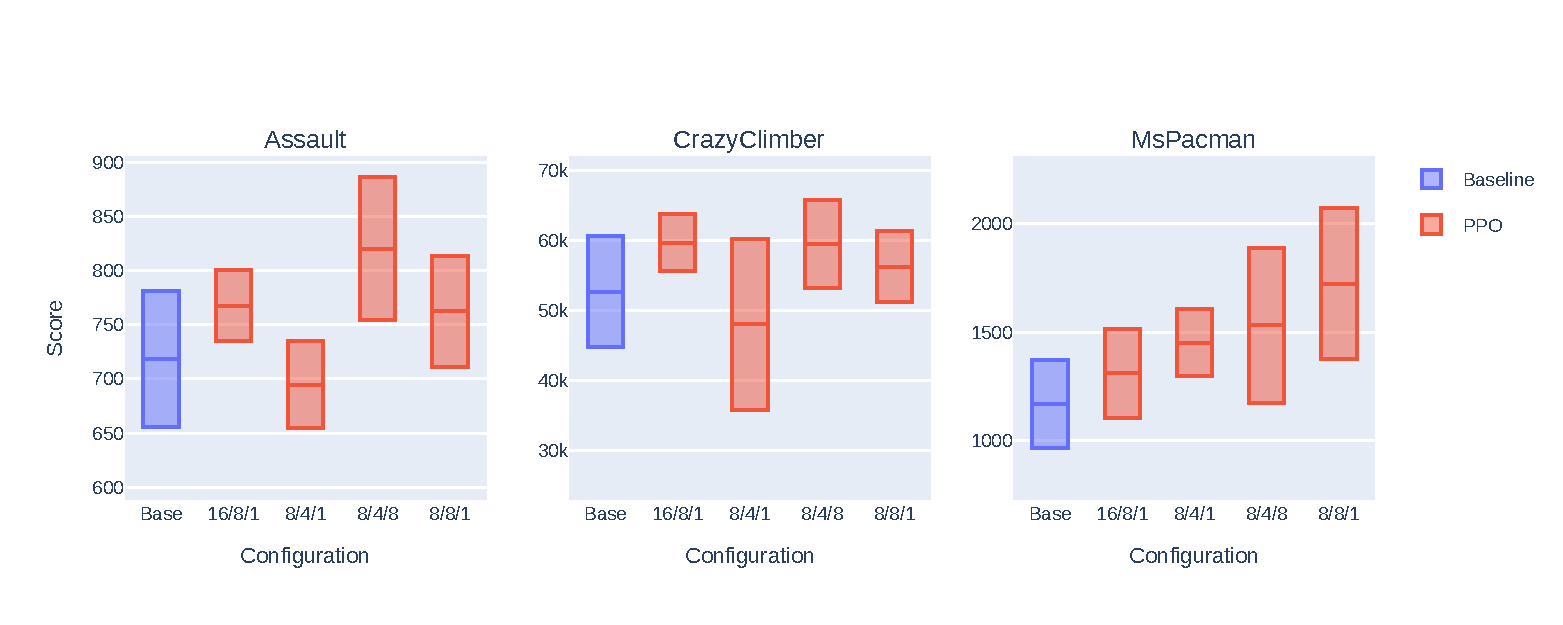
\includegraphics[width=\figurewidth,height=\figureheight,keepaspectratio]{assets/ppo.sweep.pdf}
  \caption{Comparison of the final validation scores between the baseline and a number of different configurations of PPO. Each subplot contains the results for a different Atari environment. Each box represents the mean and the standard deviation computed across $5$ training runs.}
  \label{fig:ppo_sweep}
\end{figure}

\begin{figure}
  \centering
  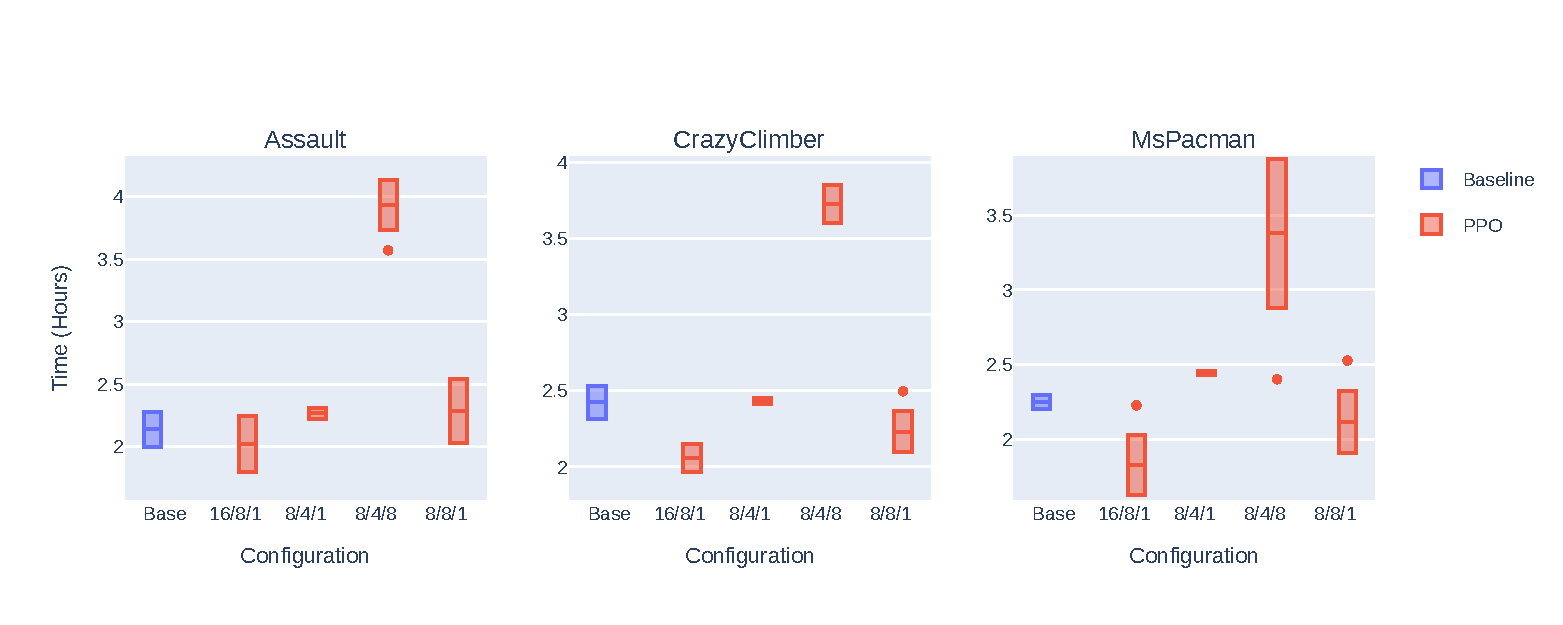
\includegraphics[width=\figurewidth,height=\figureheight,keepaspectratio]{assets/ppo_sweep.time.pdf}
  \caption{Comparison of the total training run durations for the baseline and a number of different configurations of PPO. Each subplot contains the results for a different Atari environment. Each box represents the mean and the standard deviation computed across $5$ training runs.}
  \label{fig:ppo_sweep_time}
\end{figure}

\subsection{SAC Experiments}

Let us now conduct the experiments with SAC algorithm.

\subsubsection{Random search over the $\alpha$ coefficient}

\paragraph{Setup} A complete grid search over network architectures, optimizer parameters etc. is clearly infeasible, and the parameters are not as directly transferable as was the case with PPO. We take the approach of reusing A2C's actor architecture and optimizer, and using A2C's encoder and optimizer settings for the value function as a proxy for SAC's $Q$ functions. As both algorithms use the target functions, we copy the target $Q$ function update schedule from A2C - a full copy every $100$ optimization steps, to be precise.

The most impactful hyperparameter left, then, is the choice of temperature/reward scale $\alpha$. As the first step, we perform a random search over the value of the parameter. Ideally, we would perform a grid search, testing each value of $\alpha$ on the set of three environments and five RNG seeds. However, such an experiment would be computationally infeasible. What we do instead, rather, is the following: for each pair of the environment/task and the RNG seed, we select the value of $\alpha$ from a log-normal distribution: $\log{\alpha} \sim \mathcal{N}(\log{10^{-3}}, \log{10})$. In other words, we expect the first standard deviation to cover the interval $[10^{-4}, 10^{-2}]$. To increase the coverage, multiple $\alpha$ values can be tested for each pair. Then, we shall estimate the optimal value of $\alpha$.

\paragraph{Results} Let us start with the analysis of the final scores (\autoref{fig:sac_alpha_perf}) Interestingly, the choice of $\alpha$ regularizer does \emph{not} seem to significantly impact the performance. If we take a look at the final entropy values (\autoref{fig:sac_alpha_ent}), which ought to be the primary metric controlled by the value of $\alpha$, we may deduce that, while the value does impact the entropy (the effect can be seen most strongly on the chart concerning \env{Assault}), at a certain point we hit a lower bound of sorts, whereafter further decreasing the value of $\alpha$ does not affect it quite as strongly. The aforementioned lower entropy bound seems to be approximately $10^{-2}$ for all the environments. Another phenomenon we can discern is the policy collapse in some instances, as indicated by near-zero validation scores of some of the experiments.

\paragraph{Conclusions} The selection of SAC's $\alpha$ parameter, and the policy entropy value, do not have a significant effect on the agent performance. In some instances, agents trained with SAC appear to collapse.

\begin{figure}
  \centering
  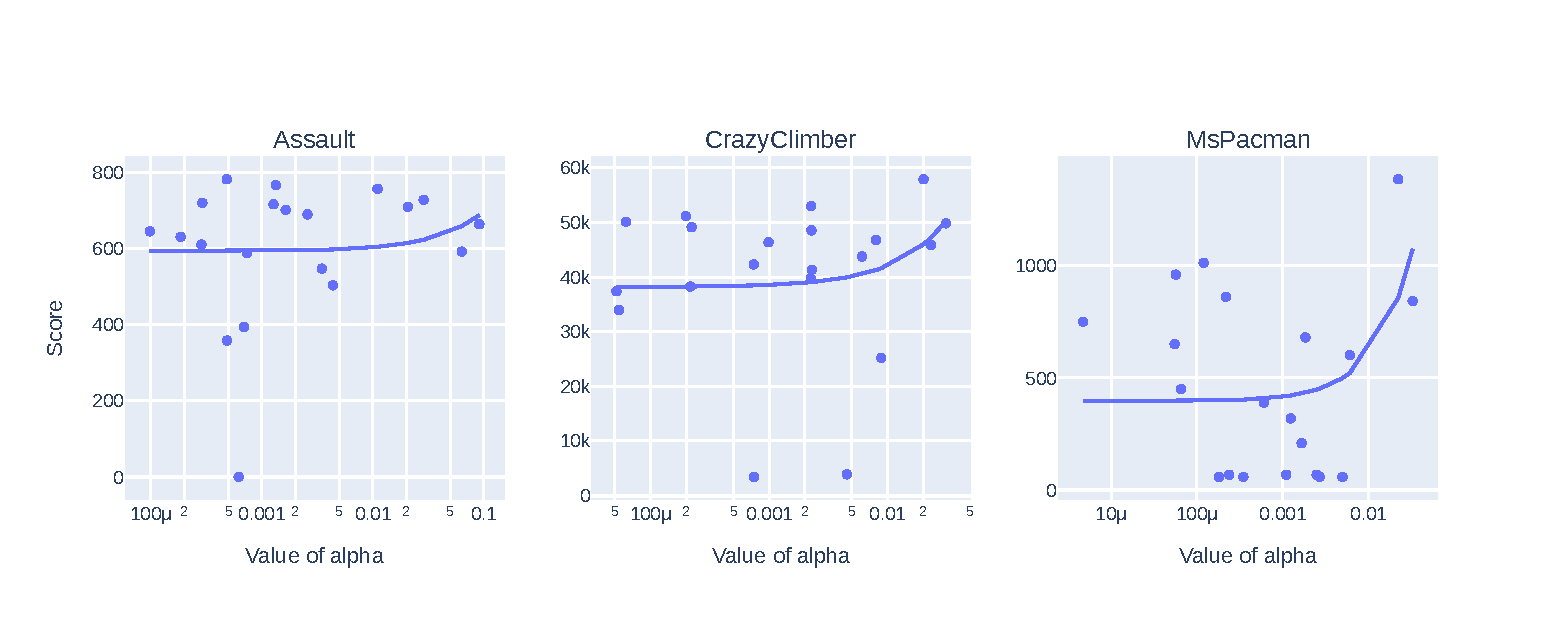
\includegraphics[width=\figurewidth,height=\figureheight,keepaspectratio]{assets/sac.alpha_perf.pdf}
  \caption{Relationship between SAC's $\alpha$ value, and the agent performance. Each subplot contains the results for a different Atari environment. Each point represents a single training run. The $x$-axis denotes the value of $\alpha$ parameter used in the test. The $y$-axis signifies the final validation score obtained by the agent.}
  \label{fig:sac_alpha_perf}
\end{figure}

\begin{figure}
  \centering
  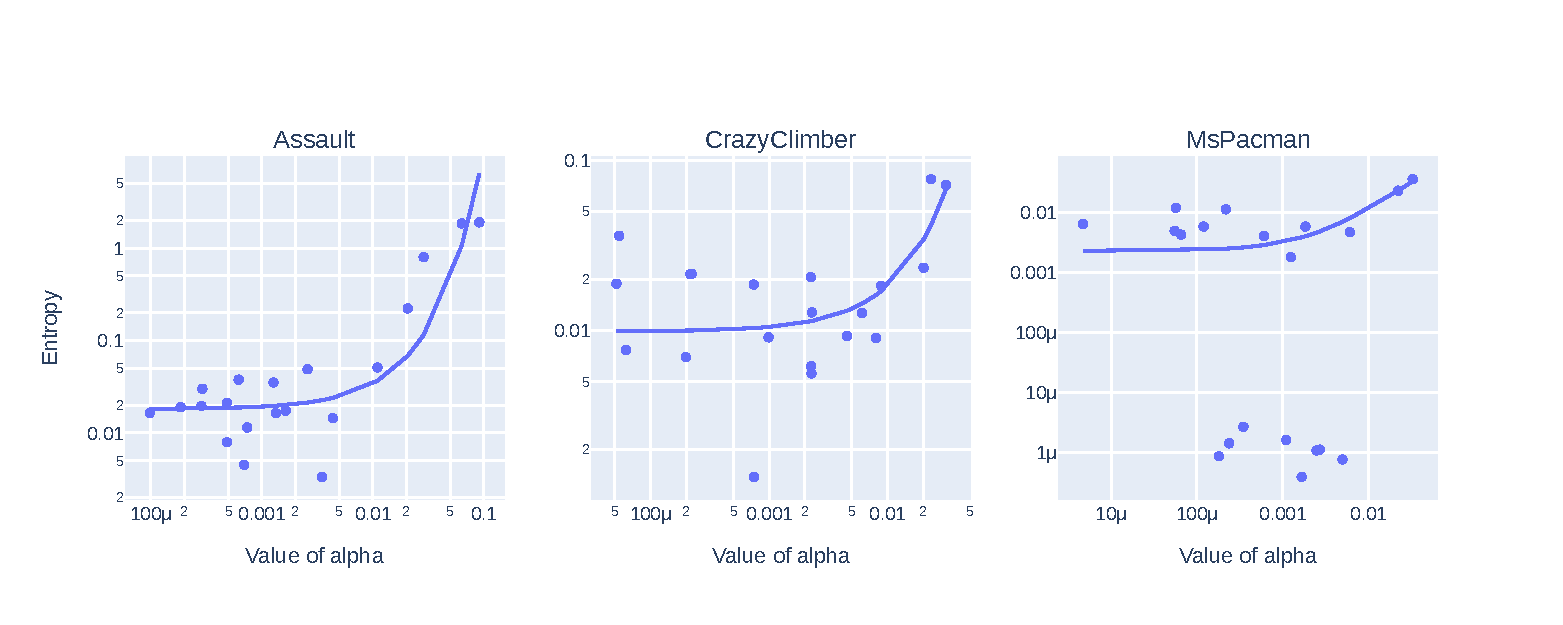
\includegraphics[width=\figurewidth,height=\figureheight,keepaspectratio]{assets/sac.alpha_ent.pdf}
  \caption{Relationship between SAC's $\alpha$ value, and the final mean policy entropy. Each subplot contains the results for a different Atari environment. Each point represents a single training run. The $x$-axis denotes the value of $\alpha$ parameter used in the test. The $y$-axis signifies the final value of the mean policy entropy metric.}
  \label{fig:sac_alpha_ent}
\end{figure}

\subsubsection{Auto-tuning $\alpha$ coefficient}

Another method, which can be used to derive the value of $\alpha$ temperature, is auto-tuning, as described in \autocite{haarnojaSoftActorCriticAlgorithms2019}. Briefly, the idea is to specify a schedule of the mean policy entropy, rather than the $\alpha$ parameter itself, and optimize the value of $\alpha$ so that the schedule is achieved. The optimization is achieved via minimization of loss function $L = \alpha (H - H_0)$, where $H_0$ denotes the current entropy target.

\paragraph{Setup} In order to use it, we must specify the target entropy schedule. The recommendations for the model-free case suggest the use of a constant entropy target of $0.89 H_{\rm max}$ for the discrete action spaces, where $H_{\rm max}$ denotes the maximum possible entropy for a policy in a given action space. However, the entropy curves of the best-performing agents in the baseline scenario (\autoref{fig:baseline_ent}) imply, that we ought to specify a rapidly decaying entropy schedule, with the final mean entropy value of approximately $0.05 H_{\rm max}$.

\begin{figure}
  \centering
  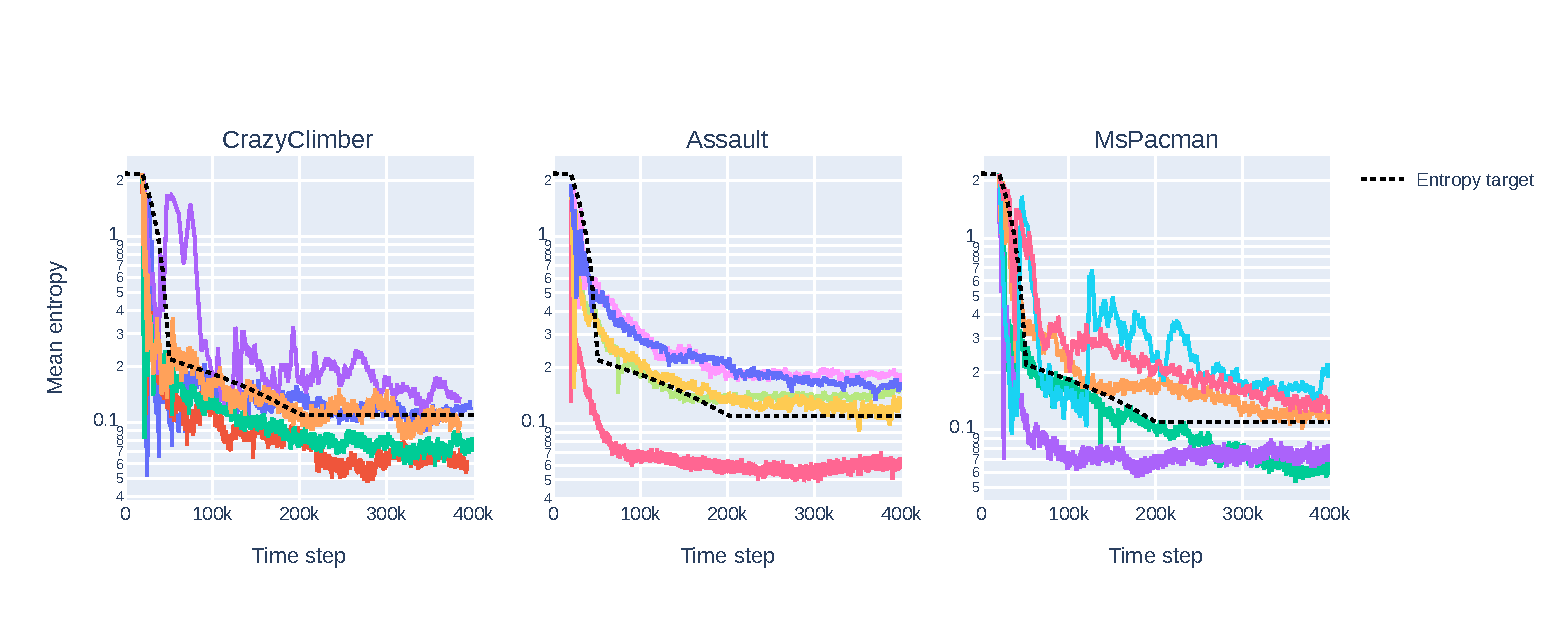
\includegraphics[width=\figurewidth,height=\figureheight,keepaspectratio]{assets/baseline_ent.pdf}
  \caption{Mean policy entropy curves for the best-performing agents in the baseline experiment. Each Atari environment is represented by a different subplot. The $x$-axis denotes the number of environment step passed. The $y$-axis represents the mean policy entropy. Each solid line represents a different training run. The dashed line denotes an example entropy schedule approximating these schedules.}
  \label{fig:baseline_ent}
\end{figure}

With this in mind, we will now proceed with an experiment, wherein we will set the entropy target to follow the dotted line on \autoref{fig:baseline_ent} - to be precise, we start at $0.99 H_{\rm max}$, descend to $0.1 H_{\rm max}$ by the environment step $50 \times 10^3$, and reach the target of $0.05 H_{\rm max}$ by the environment step $200 \times 10^3$. As for the optimizer for the $\alpha$ loss value, we choose Adam with learning rate $2.5 \times 10^{-3}$, $\epsilon = 10^{-5}$ and leave other parameters as default in Pytorch.

\paragraph{Results} The results (\autoref{fig:sac_ent_sched}) are inconclusive - performance on \env{MsPacman} is significantly improved, remains approximately the same on \env{Assault}, and is degraded on \env{CrazyClimber}.

\begin{figure}
  \centering
  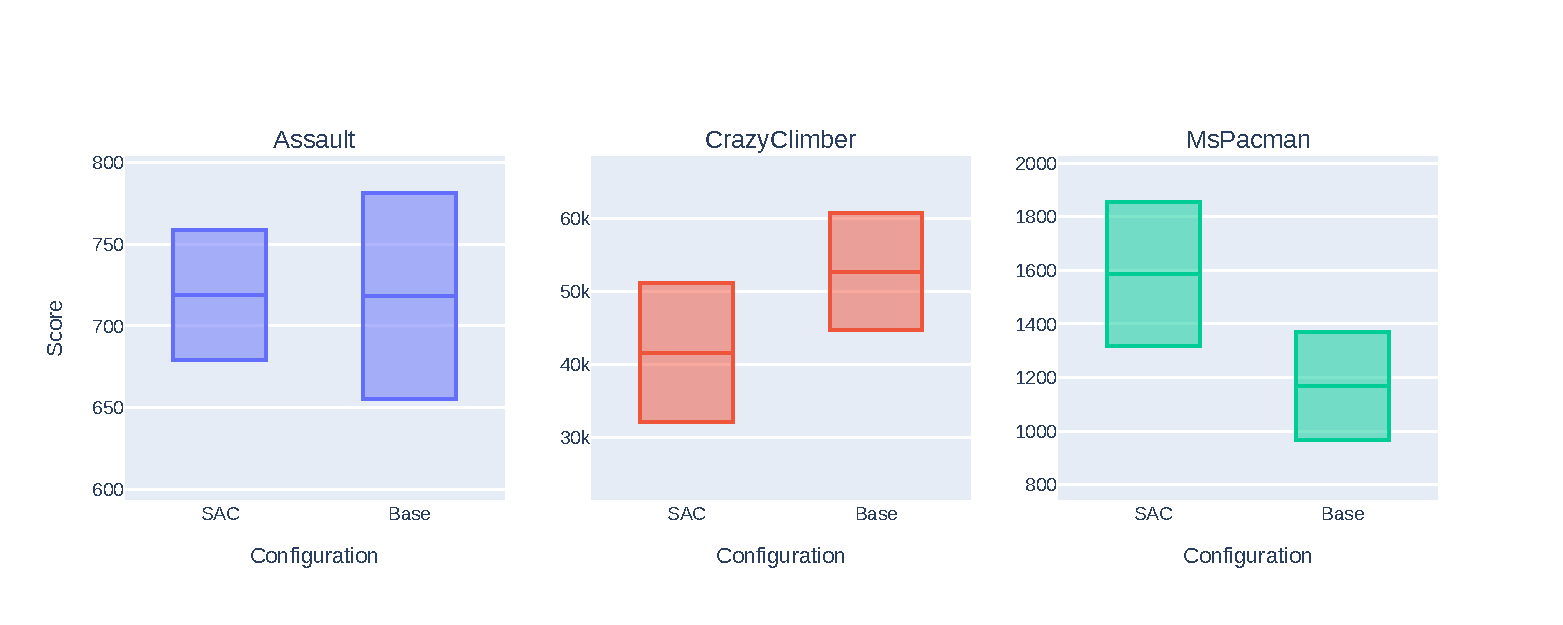
\includegraphics[width=\figurewidth,height=\figureheight,keepaspectratio]{assets/sac.ent_sched2.pdf}
  \caption{A comparison between the baseline experiment and the experiment with SAC and a user-defined entropy schedule. Each Atari environment tested is represented by a single subplot. The boxes denote the mean and the standard deviation of the final validation score, estimated with $5$ training runs per configuration.}
  \label{fig:sac_ent_sched}
\end{figure}

\subsection{CEM Experiments}

\paragraph{Setup} We base the experiment off of the baseline setup (\autoref{sec:baseline}), and replace the RL module with CEM-based planning module. Thus, the training of the RL module is unnecessary, and the agent performs a planning phase for every interaction. The configuration is fixed, with horizon length $H = 12$, optimization iterations of $I = 10$, candidate sample count of $J = 128$ and elite population of $K = 16$. We perform two sets of tests, with different values of the model/RL update ratio: $K_{\rm WM} = K_{\rm RL} = 4$ and $K_{\rm WM} = K_{\rm RL} = 8$.

\paragraph{Results} The comparison of the final validation scores (\autoref{fig:cem_base}) reveals, that the substition of the RL module by a CEM planner significantly degrades the performance of the agents on the three Atari games tested.

\begin{figure}
  \centering
  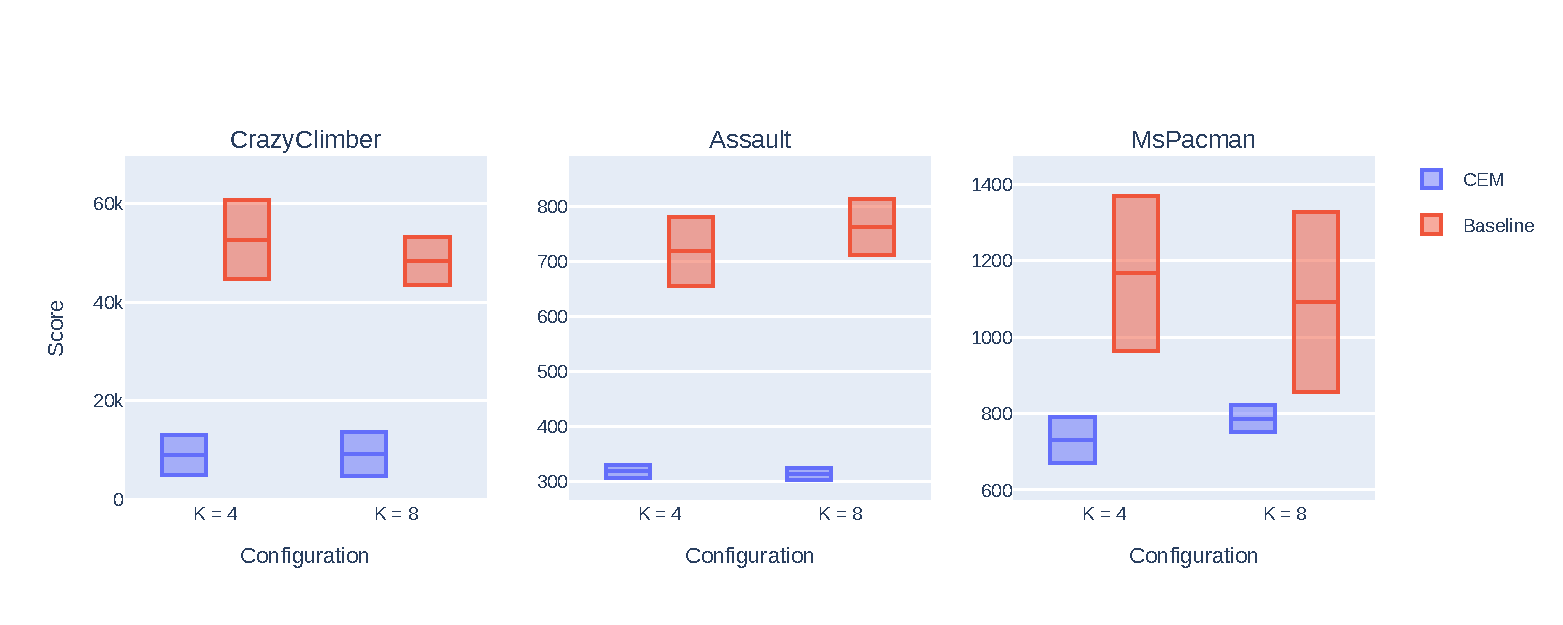
\includegraphics[width=\figurewidth,height=\figureheight,keepaspectratio]{assets/cem_base.pdf}
  \caption{A comparison of the final validation scores for the agent using CEM-based planner, and the baseline using A2C. Each subplot represents the results for a single environment. In each subplot, results for different values of model/RL update ratio $K$ are grouped together. Each group contains a box, signifying the mean and the standard deviation evaluated across $5$ training runs, for the CEM-based and A2C-based variants.}
  \label{fig:cem_base}
\end{figure}

\section{Plasticity analysis}

A number of works have identified the phenomenon of plasticity loss, meaning the inability of neural networks to learn from more recent data samples in the continual learning setting, as a possible culprit in the degradation of the RL agent performance \autocite{julianiStudyPlasticityLoss2024,nikishinPrimacyBiasDeep2022,lyleUnderstandingPlasticityNeural2023}. It might prove fruitful to investigate, whether something similar happens in the case of model-based RL, and specifically the agents based on Dreamer algorithm.

\subsection{Plasticity loss check}

In the first order, we would like to perform a ``post hoc'' test of plasticity loss - the results will not allow us to monitor the occurence of the phenomenon \emph{during} training, but will show whether the degradation has occured.

\paragraph{Setup} We follow the strategy of \autocite{julianiStudyPlasticityLoss2024}, wherein an agent is trained \emph{warm-started}, i.e. starting from the neural network parameters of a previously trained agent. In that study, the process is repeated $10$ times. Due to computational constraints, we only perform a single repetition. Also, the environments under investigation there were drawn from the Coinrun suite of randomized environment. As we are interested in Atari tasks, and there is no standard way to randomize the environment - the idea of changing the Atari game does not work due to different action spaces, meaning different agent architectures are required - we devise a custom randomization scheme for Atari. At the start of the training run, we choose (1) a particular permutation $\sigma$ of actions, meaning an action $a \in \{0, \ldots, A - 1\} =: \mathcal{A}$ is mapped to $\sigma(a) \in \mathcal{A}$; (2) with probability $50\%$, whether to flip horizontally all the video frames; (3) with probability $50\%$, whether to flip vertically all the video frames. These randomizations have been selected in order to ensure, that the warm-started agent approximately achieves the performance of a random agent, and that the observation and action statistics, e.g. the mean and standard deviation of the pixel values, remain the same.

The training recipe follows the reference test with the default DreamerV2 settings and an environment step budget of $6 \times 10^6$, also used to compare the Pytorch and Tensorflow implementations (\autoref{fig:torch_v_ref}). The choice is motivated by the smaller variance of the results compared to the time horizon of $400 \times 10^3$ used for the other experiments, making the interpretation of the results easier. We load a checkpoint from a baseline test (\autoref{sec:baseline}) with the update ratio value of $K = 1$, representing the checkpoints most affected by the primary bias. The environment used during the training run corresponding to the checkpoint is the same, but it is randomized, and we change the RNG seeds to introduce further randomization.

\paragraph{Results} The comparison of the warm-started and randomly-initialized agents (\autoref{fig:plas_check}) reveals, that, at least in some instances, the agents experience plasticity loss. To be specific, for \env{Assault} and \env{CrazyClimber}, we see either negligible or small impairment in terms of performance, whereas the effect is far more substantial for \env{MsPacman}. These findings are consistent with the analysis of the loss curves, since we have observed the stalling of the training process to be most pronounced for \env{MsPacman}. Since the degradation cannot realistically be caused by increased difficulty of the setting, having merely applied action permutations and random flips, we can only conclude that the underlying cause is primary bias.

\paragraph{Conclusions} Heavily overoptimized agents can be affected by plasticity loss. The effect is, however, not consistent.

\begin{figure}
  \centering
  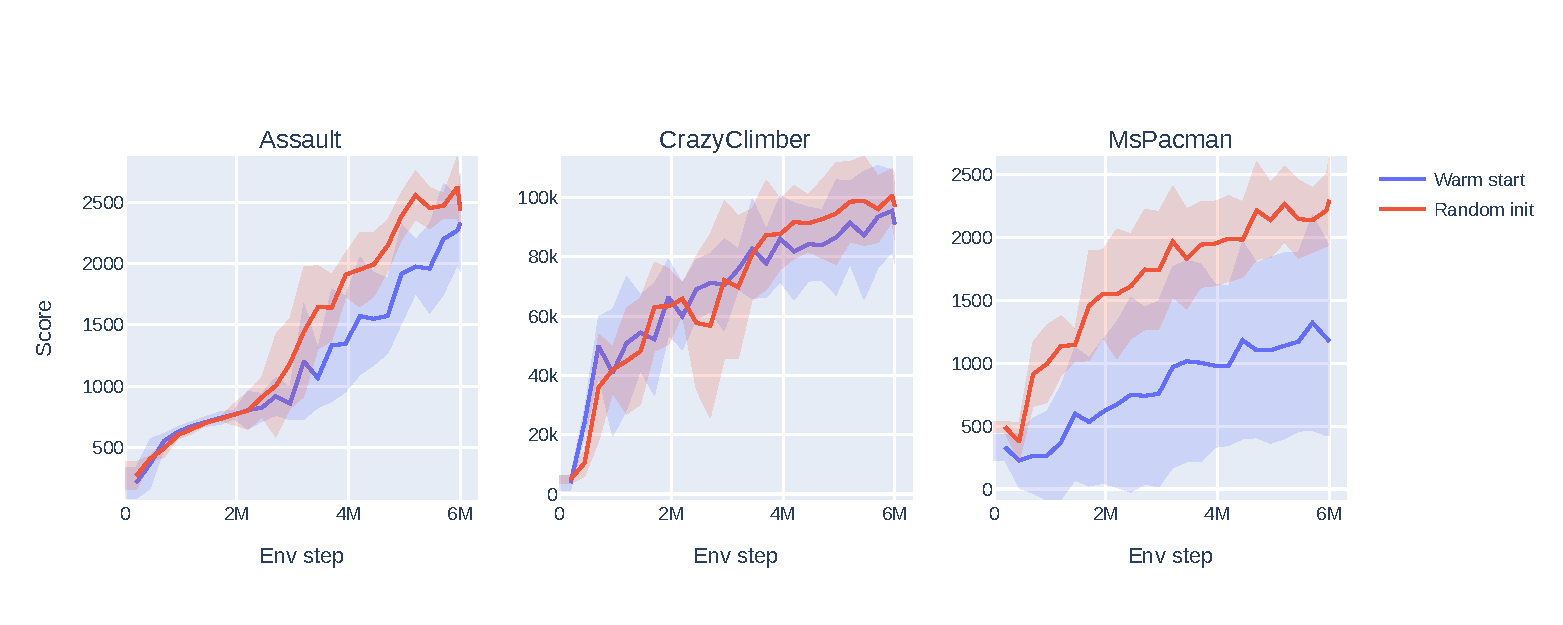
\includegraphics[width=\figurewidth,height=\figureheight,keepaspectratio]{assets/plas_check.pdf}
  \caption{A comparison of the validation scores for the warm-started agents, and the ones with parameters initialized randomly. The lines show the mean and the standard deviation of agent validation scores, measured across 5 RNG seeds.}
  \label{fig:plas_check}
\end{figure}

\subsection{Metrics related to plasticity loss}

A number of factors have been recognized as being potentially indicative of plasticity loss. We follow suggestion of \autocite{julianiStudyPlasticityLoss2024} to test weight magnitude increase and the number of dead activation units, the latter being the number of activation units which have saturated, e.g. never produce non-negative outputs for ReLU units.

We will specifically look at the relationship between these values at the end of training run for the source checkpoint, and the performance in the randomized setting. We find (\autoref{fig:plas_check_metrics}) no clear correlation between these metrics and the performance achieved in the warm-started training run. This appears consistent with prior work \autocite{lyleUnderstandingPlasticityNeural2023}, in which various plausible explanations of why neural networks may lose the ability to fit new targets over time have been found to lack explanatory power.

\begin{figure}
  \centering
  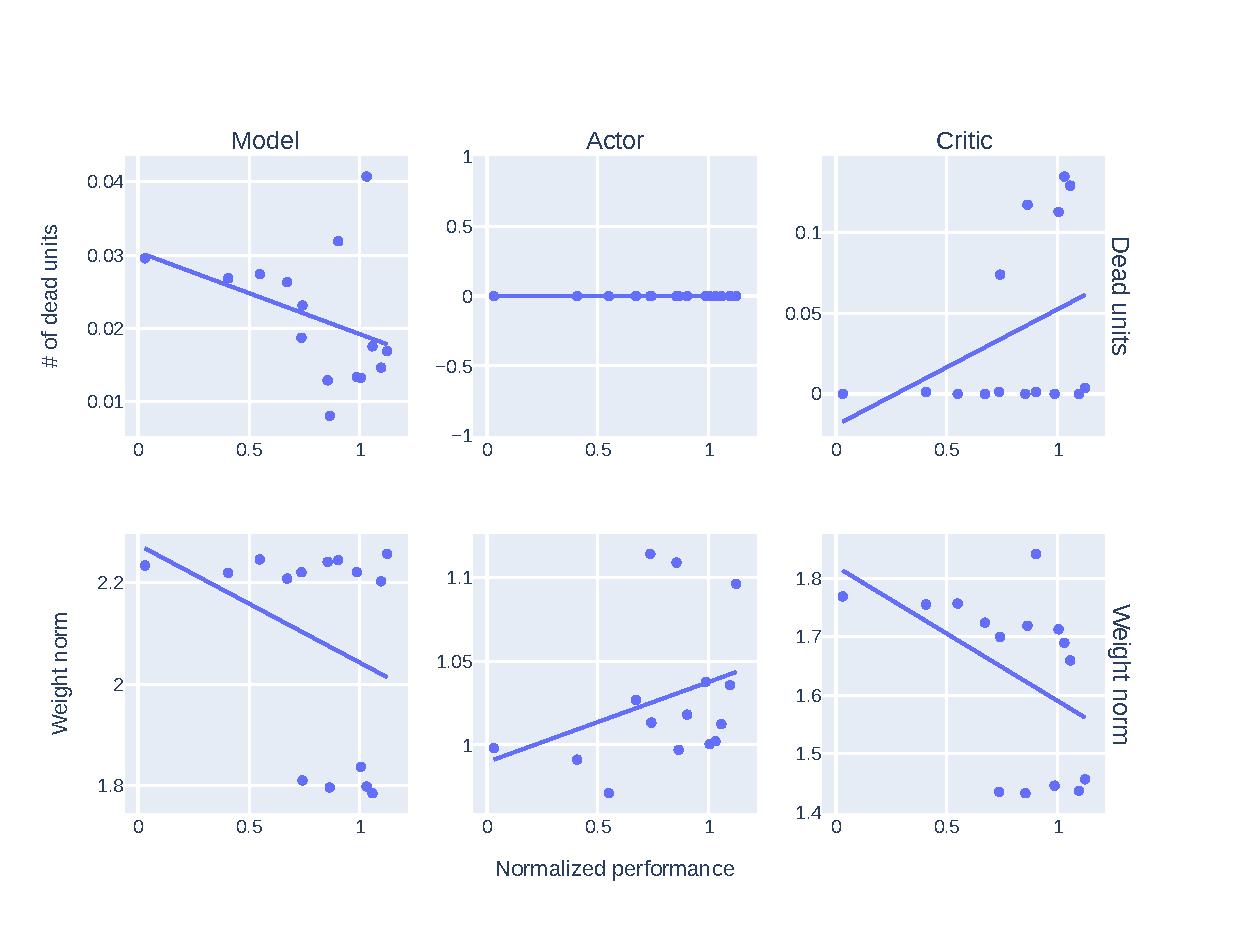
\includegraphics[width=\figurewidth,height=\figureheight,keepaspectratio]{assets/plas_check.metrics.pdf}
  \caption{Relationship between plasticity-related metrics and agent performance. Rows represent metrics used, while the columns represent the different components (neural networks) measured. The $x$-axis represents agent performance normalized by the mean score achieved in a non-warm-started setting. The $y$-axis represents values of the particular metrics.}
  \label{fig:plas_check_metrics}
\end{figure}

\subsection{A comment on the possible interventions}

In works such as \autocite{doroSampleEfficientReinforcementLearning2022,schwarzerBiggerBetterFaster2023}, periodic resets of the parameters have been used with great effect to counteract the plasticity loss. Although an auto-reset scheme may perhaps be possible to construct, we consider such an investigation to be out-of-scope for this thesis, due to aforementioned lack of clear indicators of it occuring. Thus, due to the extent of required hyperparameter optimization and the inability to reduce it through automated methods, we decide not to pursue adding periodic resets to the developed agent. It is, however, an interesting avenue for further improvements in terms of sample efficiency of MBRL agents.

\section{Combining the improvements}

Our experiments have singled out two major avenues for improvement, insofar as the agent performance is concerned: the adaptive update ratio schema, and the use of PPO instead of the default A2C. We have, however, tested them in isolation. It remains for us to see what happens if we employ them all at once. We shall also see the effect of these ablations on the 23 unseen environments.

Due to the requisite computational resources required to run the entire benchmark (26 games $\times$ 5 RNG seeds per single configuration), we will first examine the effects on the three test environments, select the hyperparameters to be used, and then run the benchmark on the chosen set.

\subsection{Hyperparameter selection}

\paragraph{Setup} In reference to the adaptive ratio system, the results suggest the use of a decoupled setup, wherein the RL update ratio is fixed. The performance gain is, however, dependent on the specific update ratio used. The validation scores obtained in the PPO experiment, on the other hand, indicate the use of either {\tt 16/8/1} or {\tt 8/8/1} configuration, the configuration name $K_{\rm RL}/N/M$ denoting the RL optimization ratio, number of PPO epochs and number of PPO minibatches respectively. We exclude the experiments with $M > 1$ due to excessive adverse effect on the training speed, despite possibly yielding improved results.

These findings suggest a following setup: we will set the RL update ratio fixed, making the model update frequency alone adaptive, and focus on the hyperparameters for the PPO. We will test a slightly wider range of presets: {\tt 8/8/1}, {\tt 16/8/1}, {\tt 4/8/1} and {\tt 8/4/1}.

\paragraph{Results} The scores obtained by the agents (\autoref{fig:final_prelim}) appear inconclusive. None of the tested presets consistently outperforms the other ones - for example, {\tt 4/8} is the best on \env{MsPacman}, {\tt 8/4} on \env{Assault} and {\tt 16/8} on \env{CrazyClimber}. Another question that arises is whether the combination of the two improvements has yielded even better results, or, in other words, whether there has been any synergy between them. To this end, let us compare the results for the adaptive ratio, PPO and their combination side by side. As we can see (\autoref{fig:final_prelim_comp}), the integrated agent does \emph{not} necessarily outperform the individual modifications. For example, on \env{MsPacman}, the PPO-only set of agents seem to achieve higher validation scores than the agents also utilizing the adaptive model ratios. It does, on the other hand, appear to slightly improve the overall results for the \env{Assault} and \env{CrazyClimber} Atari environments.

\begin{figure}
  \centering
  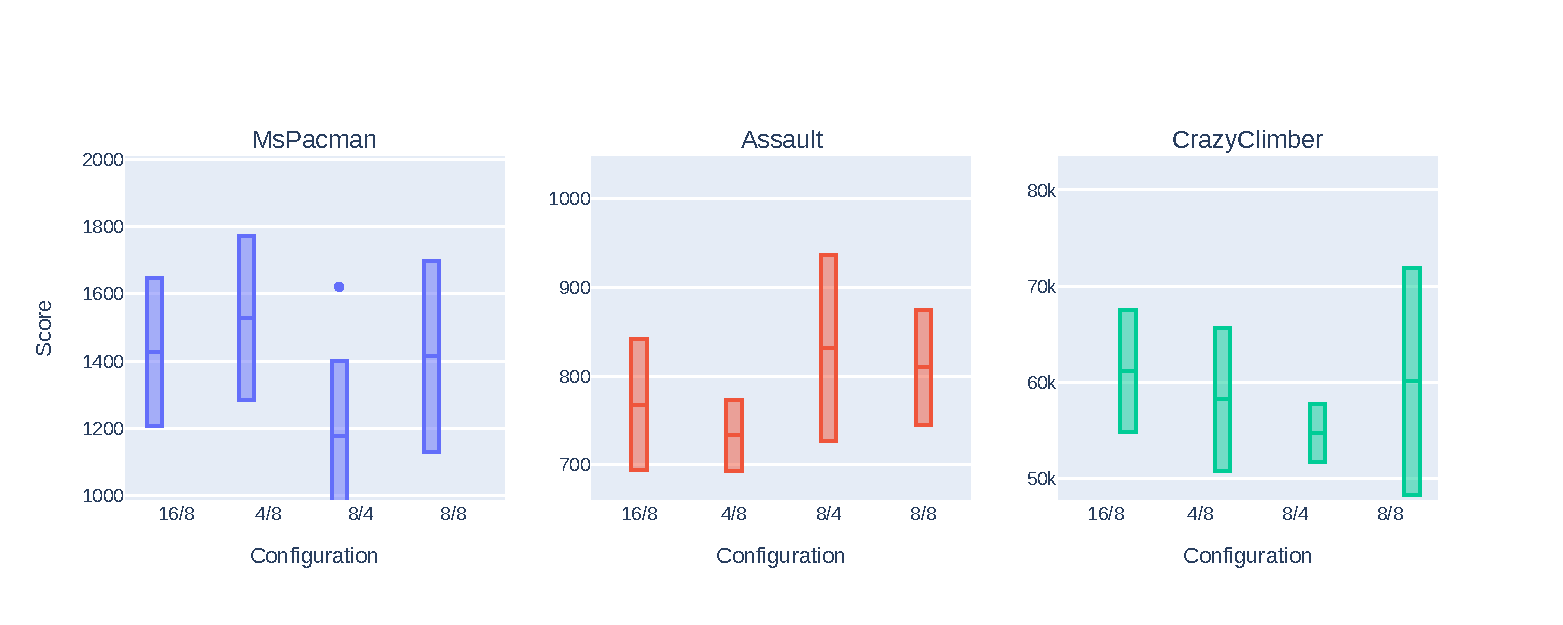
\includegraphics[width=\figurewidth,height=\figureheight,keepaspectratio]{assets/final_prelim.pdf}
  \caption{A comparison between the different hyperparameter presets for the experiment combining improvements in the context of a single agent.}
  \label{fig:final_prelim}
\end{figure}

\begin{figure}
  \centering
  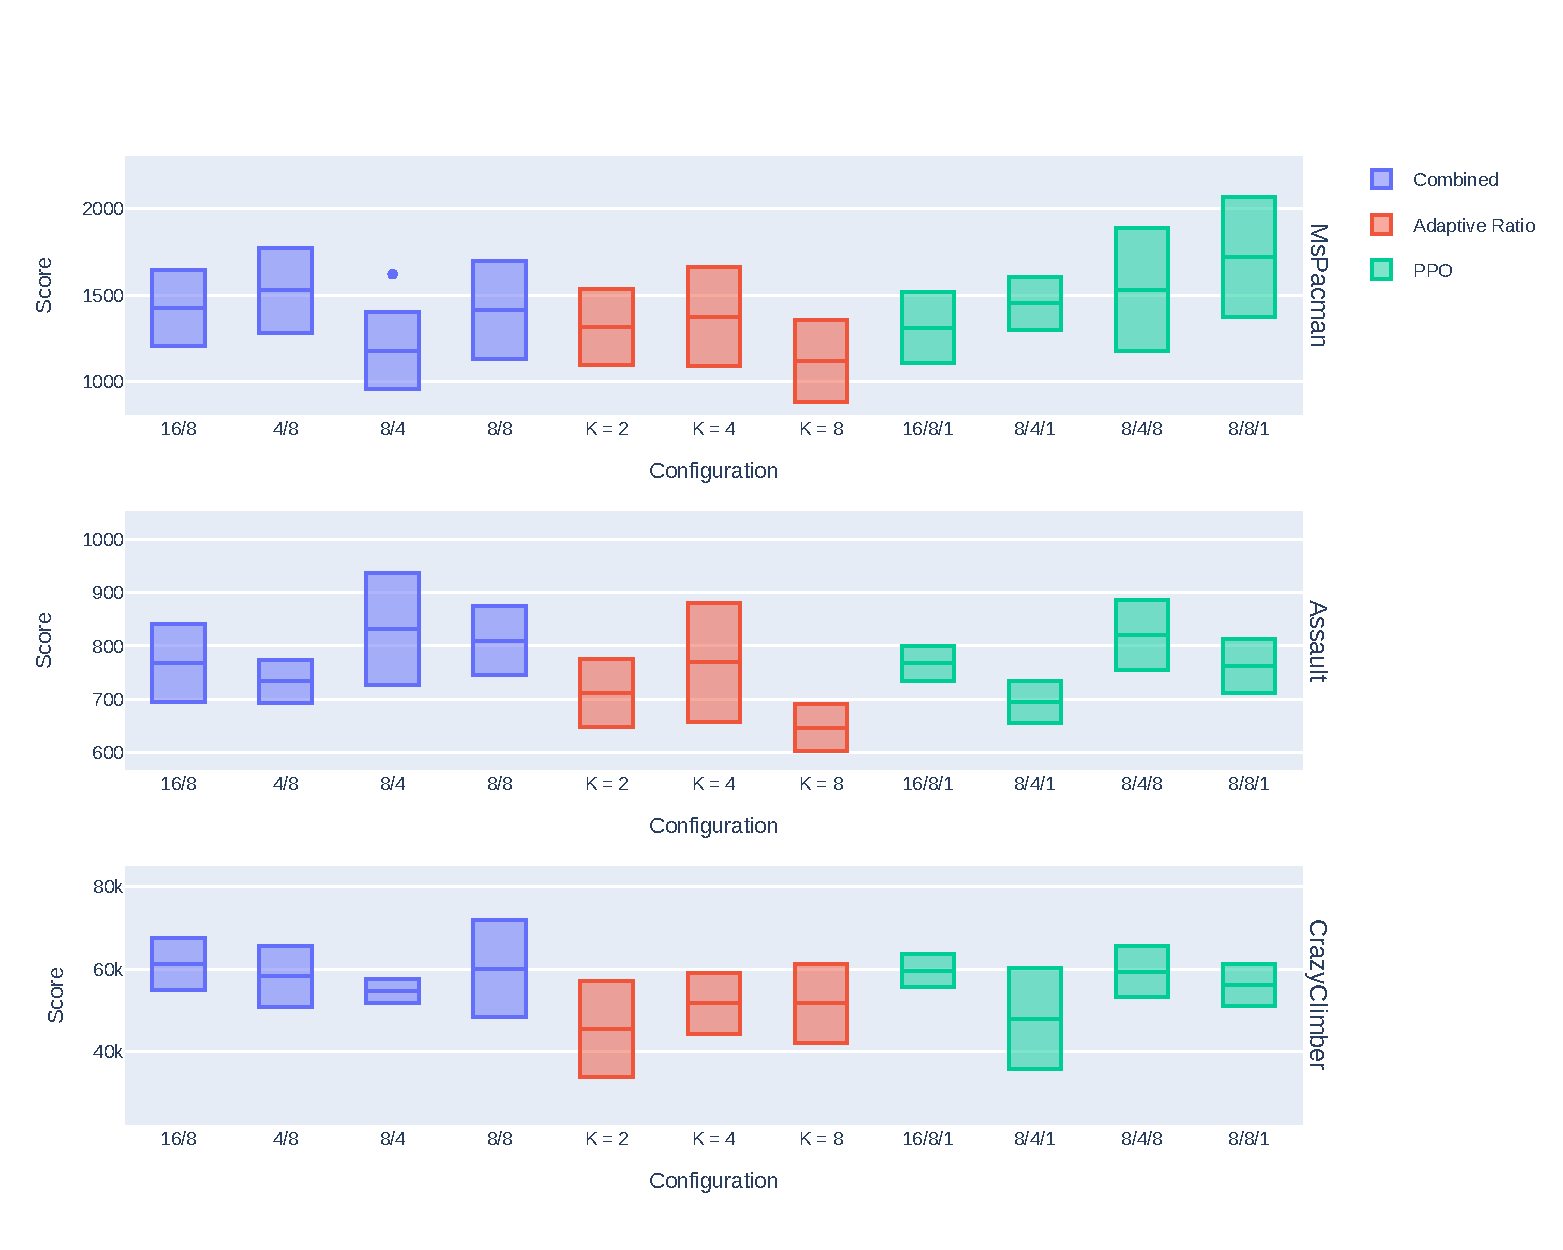
\includegraphics[width=\figurewidth,height=\figureheight,keepaspectratio]{assets/final_prelim_comp.pdf}
  \caption{A comparison between the results for the adaptive ratio, PPO and their combination. Each row represents a single Atari environment. The boxes, denoting the mean and standard deviation computed across 5 RNG seeds, are placed into three groups, corresponding to the combined test, adaptive model ratio, and PPO. Each box in a given group corresponds to a different hyperparameter preset.}
  \label{fig:final_prelim_comp}
\end{figure}

A more quantitative comparison (\autoref{tab:final_prelim_tab}) supports the choice of either the preset $K_{\rm RL} = 8, N = 8$, or $K_{\rm RL} = 8, N = 4$, with both PPO and the adaptive model update ratio used, depending on whether we want to maximize mean or median human-normalized scores. In our estimation, the former configuration is more appropriate, due to lower gap between the mean and the median values.

\begin{table}
  \centering
  \begin{adjustbox}{width=1.0\textwidth}
    \begin{tabular}{lllllll}
\toprule
 &  & \multicolumn{3}{r}{Environment} & \multicolumn{2}{r}{Human Norm} \\
 &  & Assault & CrazyClimber & MsPacman & Mean & Median \\
Ablation & Preset &  &  &  &  &  \\
\midrule
\multirow[t]{3}{*}{Adaptive} & K = 2 & 711 & 45460 & 1317 & 0.83 & 0.94 \\
 & K = 4 & 769 & 51691 & 1374 & 0.95 & 1.05 \\
 & K = 8 & 646 & 51694 & 1117 & 0.86 & 0.82 \\
\cline{1-7}
\multirow[t]{4}{*}{Combined} & 16/8 & 767 & {\bf 61163} & 1426 & 1.08 & 1.05 \\
 & 4/8 & 733 & 58230 & 1528 & 1.02 & 0.98 \\
 & 8/4 & {\bf 831} & 54714 & 1176 & 1.02 & {\bf 1.17} \\
 & 8/8 & 809 & 60104 & 1414 & {\bf 1.09} & 1.13 \\
\cline{1-7}
\multirow[t]{4}{*}{PPO} & 16/8/1 & 767 & 59651 & 1311 & 1.05 & 1.05 \\
 & 8/4/1 & 694 & 48020 & 1451 & 0.86 & 0.91 \\
 & 8/4/8 & 820 & 59431 & 1531 & 1.09 & 1.15 \\
 & 8/8/1 & 762 & 56237 & {\bf 1723} & 1.02 & 1.04 \\
\cline{1-7}
\bottomrule
\end{tabular}
}
  \end{adjustbox}
  \caption{A numerical comparison of the results for different ablation types and hyperparameter presets. The middle three columns, under the header ``Environment'' contain the mean final validation scores. The rightmost two columns denote the human-normalized median and mean scores computed across the three environments. The bold font indicates highest values in each category.}
  \label{tab:final_prelim_tab}
\end{table}

\subsection{Atari-100k benchmark}

Now, we are in the position to perform the complete Atari-100k benchmark, consisting of 26 environments, as opposed to the subset of 3 video games most predictive of the overall performance investigated so far.

\paragraph{Setup} We follow standard environment settings described in \autocite{kaiserModelBasedReinforcementLearning2024}. The main difference between the regular configuration is that for $200\times 10^6$ environment steps, \emph{sticky actions} are used, meaning an action is repeated with probability $p=0.25$, whereas for Atari-100k benchmark, they are disabled. For each of the 26 Atari games, we perform $5$ training runs, with different RNG seeds.

\paragraph{Results} The comparison  can be found in \autoref{tab:atari_100k_scores}. We compare our agent's performance with a selection of sample-efficient architectures, both model-based (SimPLe, TWM, IRIS, DreamerV3), model-free (SR-SPR, BBF) and utilizing look-ahead search (EfficientZero). The per-environment and aggregate human-normalized median and mean scores have been taken from \autocite{hafnerMasteringDiverseDomains2024} and \autocite{schwarzerBiggerBetterFaster2023}.

Overall, the agent does not attain state-of-the-art performance, but, we argue, it performs better than might perhaps be expected. If we look at the human-normalized mean scores, we can see, that our method reaches performance comparable with Transformer-based IRIS model, and exceeding TWM, significantly smaller compute requirements. We also attain highest performance of all the games tested on two environments (\env{Freeway} and \env{Krull}).

Compared with the base DreamerV2, with a time budget of $200 \times 10^6$ frames (\autoref{fig:dreamerv2_curves}), we reach the performance of the original agent at $3 \times 10^6$ environment steps, indicating an overall speedup of $7.5 \times$. Notably, the speedup factor is the same for both human-normalized mean and median scores, which helps explain the disparity between the mean and the median performance - even with a budget of $200 \times 10^6$, being $500\times$ higher than is the case for Atari-100k, the human-normalized median performance is only $\approx 1.8$, and the median performance of BBF is reached at $\approx 23 \times 10^6$ environment steps. With a different underlying world model, the median performance could be improved; our framework makes such ablations easy to conduct.

\begin{table}
  \centering
  \begin{adjustbox}{width=1.0\textwidth}
    \begin{tabular}{l|rr|rrrrrrrr|r}
    \toprule
    Environment    & Random & Human & SimPLe & TWM   & IRIS  & DreamerV3 & SR-SPR     & EffZero   & BBF       & DreamerV2 & Ours     \\
    \midrule
    Alien          & 228    & 7128  & 617    & 675   & 420   & 1118      & 1108       & 808       & \bf 1173  & 378       & 708      \\
    Amidar         & 6      & 1720  & 74     & 122   & 143   & 97        & 203        & 149       & \bf 245   & 43        & 98       \\
    Assault        & 222    & 742   & 527    & 683   & 1524  & 683       & 1089       & 1263      & \bf 2098  & 391       & 881      \\
    Asterix        & 210    & 8503  & 1128   & 1117  & 854   & 1062      & 903        & \bf 25558 & 3946      & 254       & 825      \\
    BankHeist      & 14     & 753   & 34     & 467   & 53    & 398       & 532        & 351       & \bf 733   & 11        & 208      \\
    BattleZone     & 2360   & 37188 & 4031   & 5068  & 13074 & 20300     & 17671      & 13871     & \bf 24460 & 3088      & 2312     \\
    Boxing         & 0      & 12    & 8      & 78    & 70    & 82        & 46         & 53        & \bf 86    & 26        & 63       \\
    Breakout       & 2      & 30    & 16     & 20    & 84    & 10        & 26         & \bf 414   & 371       & 1         & 3        \\
    ChopperCommand & 811    & 7388  & 979    & 1697  & 1565  & 2222      & 2362       & 1117      & \bf 7549  & 827       & 937      \\
    CrazyClimber   & 10780  & 35829 & 62584  & 71820 & 59324 & \bf 86225 & 45544      & 83940     & 58432     & 26273     & 77748    \\
    DemonAttack    & 152    & 1971  & 208    & 350   & 2034  & 577       & 2814       & 13004     & \bf 13341 & 63        & 128      \\
    Freeway        & 0      & 30    & 17     & 24    & 31    & 0         & 25         & 22        & 26        & 19        & \bf 32   \\
    Frostbite      & 65     & 4335  & 237    & 1476  & 259   & \bf 3377  & 2585       & 296       & 2385      & 175       & 251      \\
    Gopher         & 258    & 2412  & 597    & 1675  & 2236  & 2160      & 712        & \bf 3260  & 1331      & 365       & 1551     \\
    Hero           & 1027   & 30826 & 2657   & 7254  & 7037  & \bf 13354 & 8524       & 9316      & 7819      & 3249      & 6029     \\
    Jamesbond      & 29     & 303   & 100    & 362   & 463   & 540       & 389        & 517       & \bf 1130  & 39        & 152      \\
    Kangaroo       & 52     & 3035  & 51     & 1240  & 838   & 2643      & 3632       & 724       & \bf 6615  & 49        & 3434     \\
    Krull          & 1598   & 2666  & 2205   & 6349  & 6616  & 8171      & 5912       & 5663      & 8223      & 4081      & \bf 9130 \\
    KungFuMaster   & 258    & 22736 & 14862  & 24555 & 21760 & 25900     & 18649      & \bf 30945 & 18992     & 16592     & 14549    \\
    MsPacman       & 307    & 6952  & 1480   & 1588  & 999   & 1521      & 1574       & 1281      & \bf 2008  & 715       & 1443     \\
    Pong           & -21    & 15    & 13     & 19    & 15    & -4        & 3          & \bf 20    & 17        & -21       & 5        \\
    PrivateEye     & 25     & 69571 & 35     & 87    & 100   & \bf 3238  & 98         & 97        & 40        & 10        & -317     \\
    Qbert          & 164    & 13455 & 1289   & 3331  & 746   & 2921      & 4044       & \bf 14448 & 4447      & 322       & 1394     \\
    Seaquest       & 68     & 42055 & 683    & 774   & 661   & 962       & 819        & 1100      & \bf 1232  & 315       & 476      \\
    UpNDown        & 533    & 11693 & 3350   & 15982 & 3546  & 46910     & \bf 112450 & 17264     & 12102     & 7420      & 24554    \\
    \midrule
    Human Median   & 0.000  & 1.000 & 0.130  & 0.510 & 0.289 & 0.490     & 0.685      & 1.116     & 0.917     & 0.024     & 0.205    \\
    Human Mean     & 0.000  & 1.000 & 0.330  & 0.960 & 1.046 & 1.250     & 1.272      & 1.945     & 2.247     & 0.305     & 0.975    \\
    \bottomrule
\end{tabular}
}
  \end{adjustbox}
  \caption{A comparison of Atari-100k scores for different RL agent architectures. \emph{Note:} The scores for DreamerV2 were computed with our framework, since the authors did not check the performance on the benchmark.}
  \label{tab:atari_100k_scores}
\end{table}

\begin{figure}
  \centering
  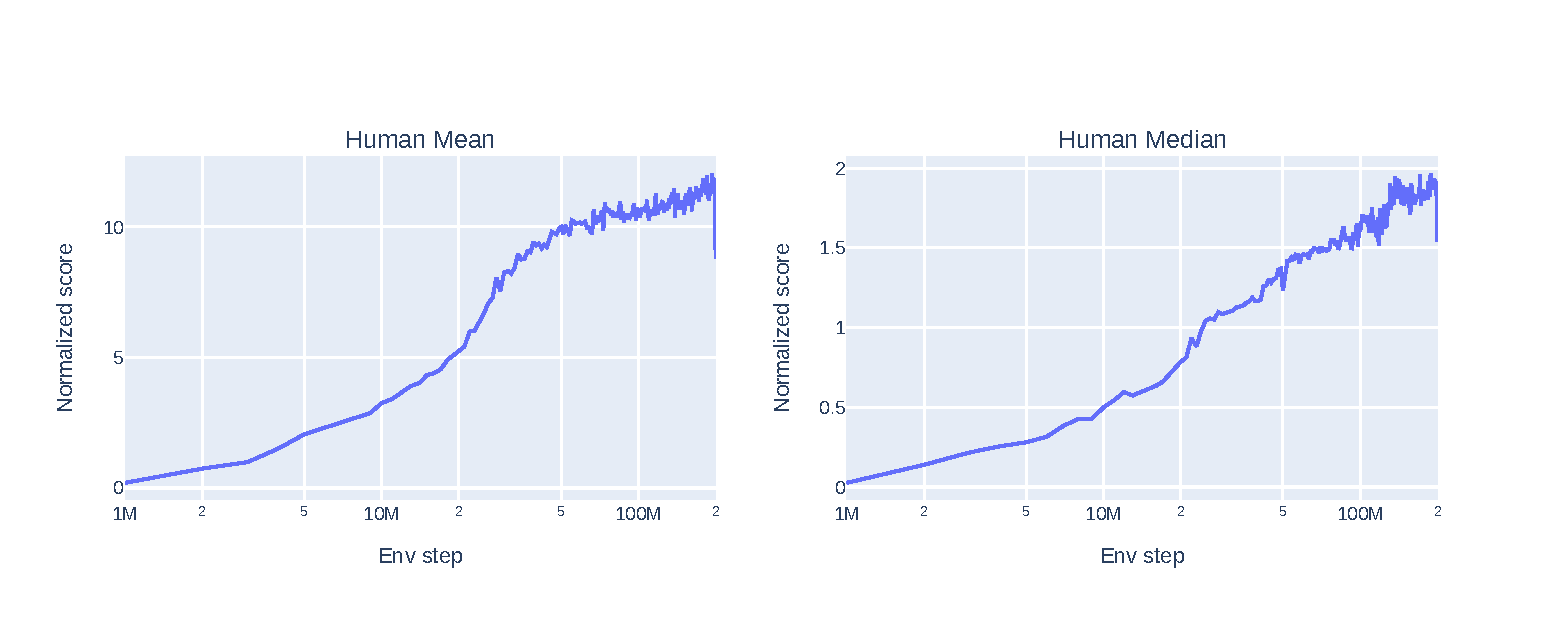
\includegraphics[width=\figurewidth,height=\figureheight,keepaspectratio]{assets/dreamerv2_curves.pdf}
  \caption{Validation score curves for base DreamerV2 agent, with a time budget of $200 \times 10^6$ frames. Two subplots are present: for human-normalized mean performance, and human-normalized median performance. \emph{Note:} The $x$-axis is logarithmic}
  \label{fig:dreamerv2_curves}
\end{figure}

We also publish the validation score curves (\autoref{fig:atari_100k_curves}). On some tasks, such as \env{ChopperCommand}, \env{DemonAttack}, \env{PrivateEye} or \env{UpNDown}, the agent appears to act almost randomly. In fact, for \env{PrivateEye}, the normalized performance is \emph{negative}. For this environment and \env{ChopperCommand}, the cause appears to be overall inferior performance of base DreamerV2 world model on these. In most cases, though, the agents do not necessarily collapse - the progress is steady, but merely slow, as indicated by the low median normalized score.

\begin{figure}
  \centering
  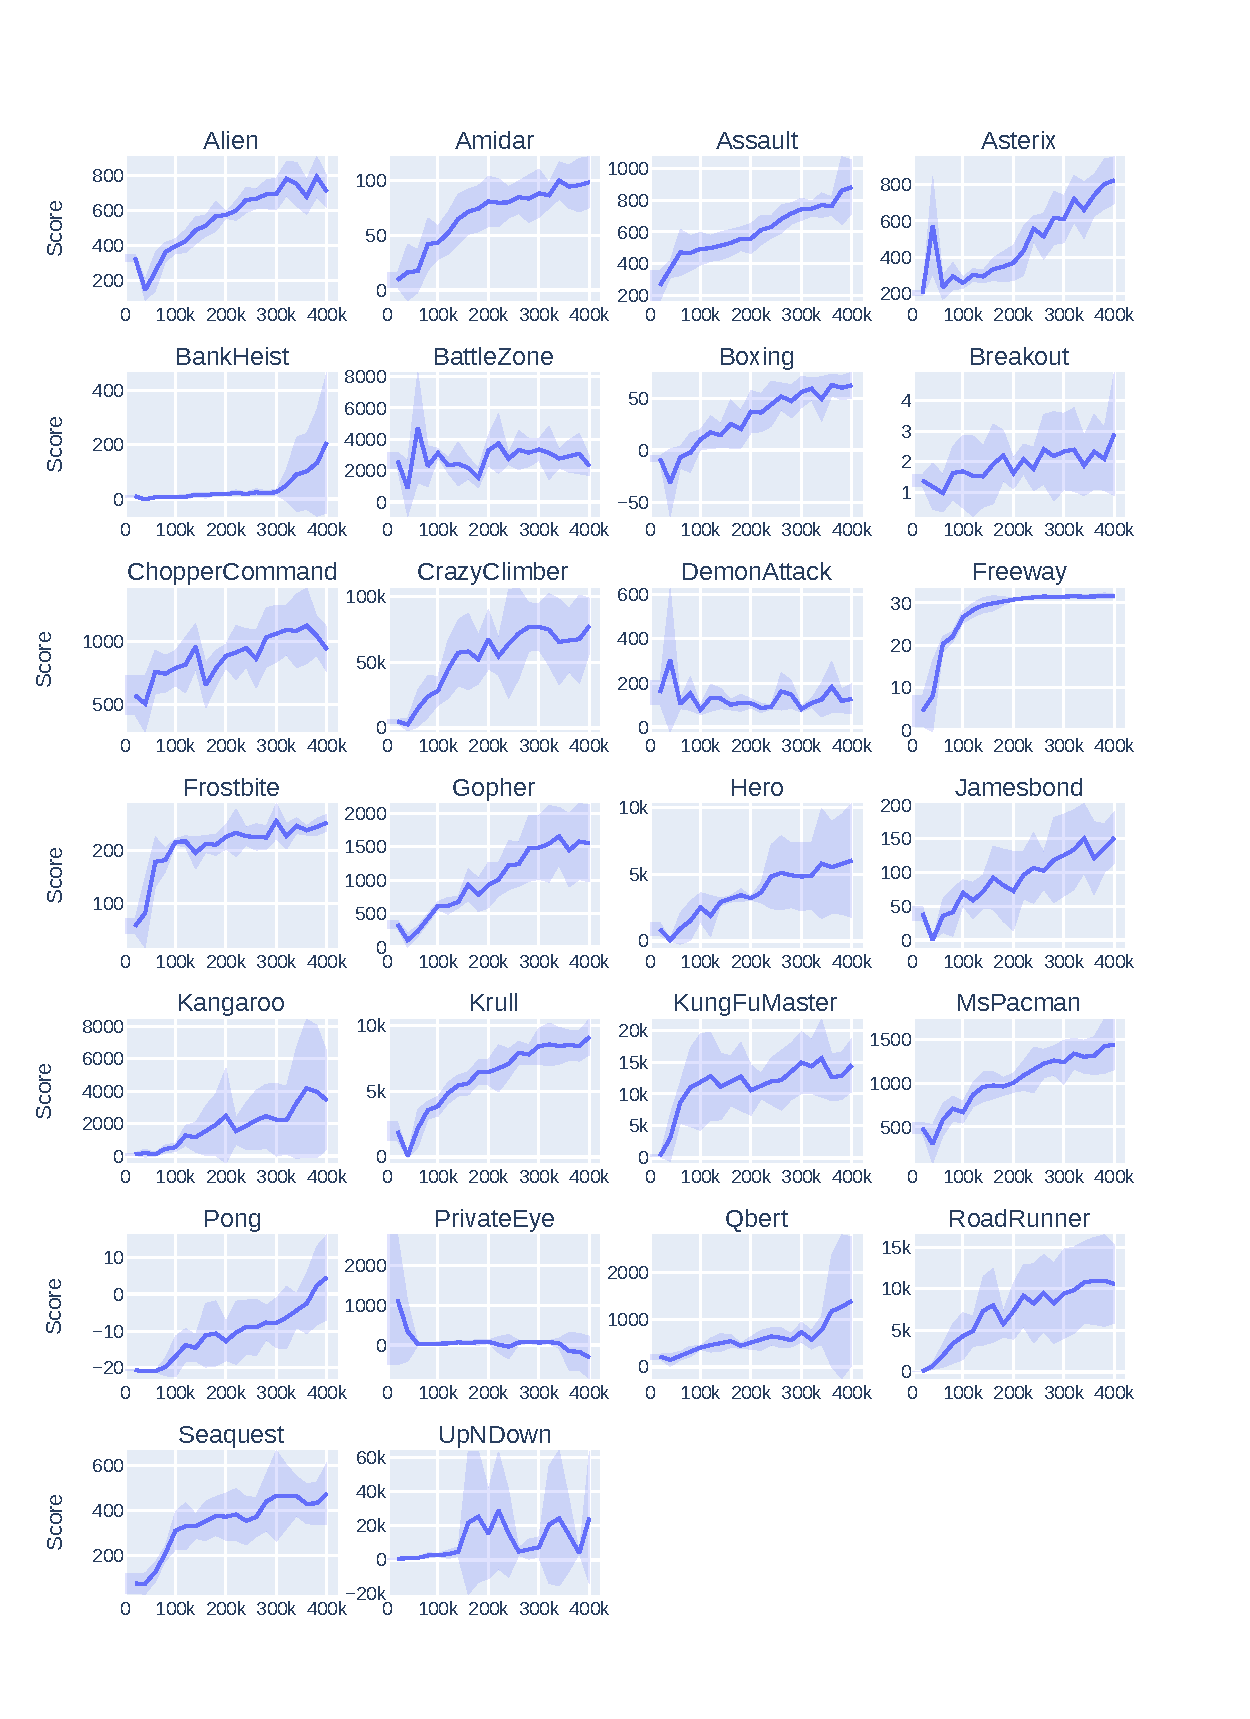
\includegraphics[width=\figurewidth,height=\figureheight,keepaspectratio]{assets/atari_100k.curves.pdf}
  \caption{Atari-100k validation score curves for our algorithm. Each subplot represents a different game from the Atari-100k benchmark. The $x$-axis denotes the environment step, and the $y$-axis the scores. The curves depict the mean and the standard deviation measured over 5 RNG seeds.}
  \label{fig:atari_100k_curves}
\end{figure}

\chapter{Discussion}

We have presented an exploration of the idea of incorporating various improvements and tweaks into a model-based RL architecture in order to make it more data-efficient. Through an extensive survey of the field, and careful agent design, we have identified the most relevant developments, and proposed an unified RL framework for combining them into a single agent.

Due to a marked lack of existing extensible and fully configurable model-based RL solutions, we have implemented a novel, open-source PyTorch-based solution, and provided a detailed analysis of the different components and software design choices, which facilitate the execution of the experiments.

In our experiments, we have demonstrated the effects of applying the ideas presented in other works in a model-based context. We have found, that some of them, such as tuning the update ratios, or experimenting with different underlying RL algorithms, have a positive effect on the agent performance, whereas others, such as the use of data augmentations, can, perhaps counterintuitively, even degrade the performance in the model-based setting. Through an in-depth analysis of the training dynamics, we have shed light on some of the phenomena at play, including the unexpected behavior of the model validation loss values.

Finally, we have examined the effects of combining the improvements, identifying a modest further performance boost, and verified the efficacy of the approach on the standard Atari-100k benchmark, finding it to be competitive with some of the current state-of-the-art approaches, despite the overall simplicity and compute efficiency of the final agent architecture. It must, however, be noted, that there remains a significant gap between algorithms using ``true'' world models without lookahead, and the algorithms either using value-equivalent models, or without their use altogether, prompting further research.

Our solution is also more compute-efficient than the alternatives. A single training run takes approximately $3.5$ hours running on half an A100 accelerator, compared with $2.4$ A100-hours for DreamerV3, $8$ A100-hours for BBF, or $3.5$ A100-\emph{days} for IRIS \autoref{tab:compute_comp}. Thus, the approach presented in our work makes work on data-efficient RL algorithms more accessible to researchers without access to massive compute resources.

An interesting avenue for future work would be to perform a more complete investigation of the plasticity loss, and to develop an automatic schema for alleviating it. Our preliminary findings suggest, that the loss of the ability to learn from recent experience in neural networks can possibly impact the performance of the model-based RL algorithms. Further network regularization via the use of weight decay or normalization layers, parameter resetting based on neuron-level staleness metrics, or architectural changes could potentially be used to automatically prevent or detect the primacy bias from occuring.

We could also attempt to better incorporate data augmentation techniques into the model-based framework. Although, in aggregate, the ablations were found to degrade the performance, we have also detected a tentative qualitative measure, the stalling of the training process, which could be utilized to adjust the strength of the augmentations, or enable/disable them altogether. One could also consider an augmentation schedule, whereby the training process would begin without any image transformations applied, and gradually start applying them as the run nears completion.

We believe, that the results presented in this thesis, as well as developed RL framework, can help further research on sample-efficient RL methods, and ultimately lead to a broader use and deployment of RL algorithms in real-world scenarios.

\section{Acknowledgements}

We would like to thank dr Cyranka for his continued support and valuable insight throughout the period of completing this thesis. This work was supported by the access to the \href{https://entropy-doc.mimuw.edu.pl/}{Entropy compute cluster}.

\printbibliography

\end{document}